 \documentclass{tufte-handout}

%--------Packages--------
\usepackage{tikz}
\usepackage{braket}
\usepackage{booktabs,tabularx,gensymb}
\usepackage{amsmath,amsfonts,amsthm,amssymb,mathrsfs,bbm}
\usetikzlibrary{calc, arrows}
\usetikzlibrary{shapes}
\usetikzlibrary{positioning}

%--------Theorem Environments--------
\newtheorem{thm}{Theorem}
\newtheorem{cor}[thm]{Corollary}
\newtheorem{lem}[thm]{Lemma}
\newtheorem{defn}[thm]{Definition}
\newtheorem{rmk}[thm]{Remark}

%--------Pseudocode--------
\usepackage{xcolor,amsmath}
\usepackage[linesnumbered,ruled,vlined]{algorithm2e}
\DontPrintSemicolon

% Define pseudocode formatting
\renewcommand{\KwSty}[1]{\textnormal{\textcolor{blue!90!black}{\ttfamily\bfseries #1}}\unskip}
\renewcommand{\ArgSty}[1]{\textnormal{\ttfamily #1}\unskip}
\SetKwComment{Comment}{\color{green!50!black}// }{}
\renewcommand{\CommentSty}[1]{\textnormal{\ttfamily\color{green!50!black}#1}\unskip}
\newcommand{\assign}{\leftarrow}
\newcommand{\var}{\texttt}
\newcommand{\FuncCall}[2]{\texttt{\bfseries #1(#2)}}
\SetKwProg{Function}{function}{}{}
\renewcommand{\ProgSty}[1]{\texttt{\bfseries #1}}

%--------Colored Theorem-------------
\usepackage[most]{tcolorbox}
\definecolor{lilac}{cmyk}{0.10, 0.20, 0, 0,0}
\tcbuselibrary{theorems}
\newtcbtheorem
  []%
  {ex}
  {\textbf{Example}}
  {%
  	breakable,
    colback=lilac!5,
    colframe=lilac!85,
    fonttitle=\bfseries,
  }% options
  {def}% prefix

%--------Shortcuts--------
\usepackage{graphicx}
\graphicspath{{./figures/}}

\newcommand{\floor}[1]{\left\lfloor #1 \right\rfloor}
\newcommand{\ceil}[1]{\left\lceil #1 \right\rceil}
\newcommand{\tabitem}{~~\llap{\textbullet}~~}
\DeclareMathOperator*{\argmax}{arg\,max}
\DeclareMathOperator*{\argmin}{arg\,min}

%--------Header--------
\title{COMP362: Honours Algorithm Design}
\author[Winter 2022]{Winter 2022}
\date{\today}

%--------Title--------
\makeatletter
\renewcommand{\maketitlepage}{%
    \cleardoublepage{%
        \begin{fullwidth}%
        \fontsize{12}{12}\selectfont\par\noindent{\@author \\ \noindent \small{Instructors: Vetta, Adrian Roshan}}%

        \vspace{5pc}%

        \fontsize{36}{40}\selectfont\par\noindent{Honours \\ \noindent Algorithm Design}%

        \vspace{2pc}%

        \noindent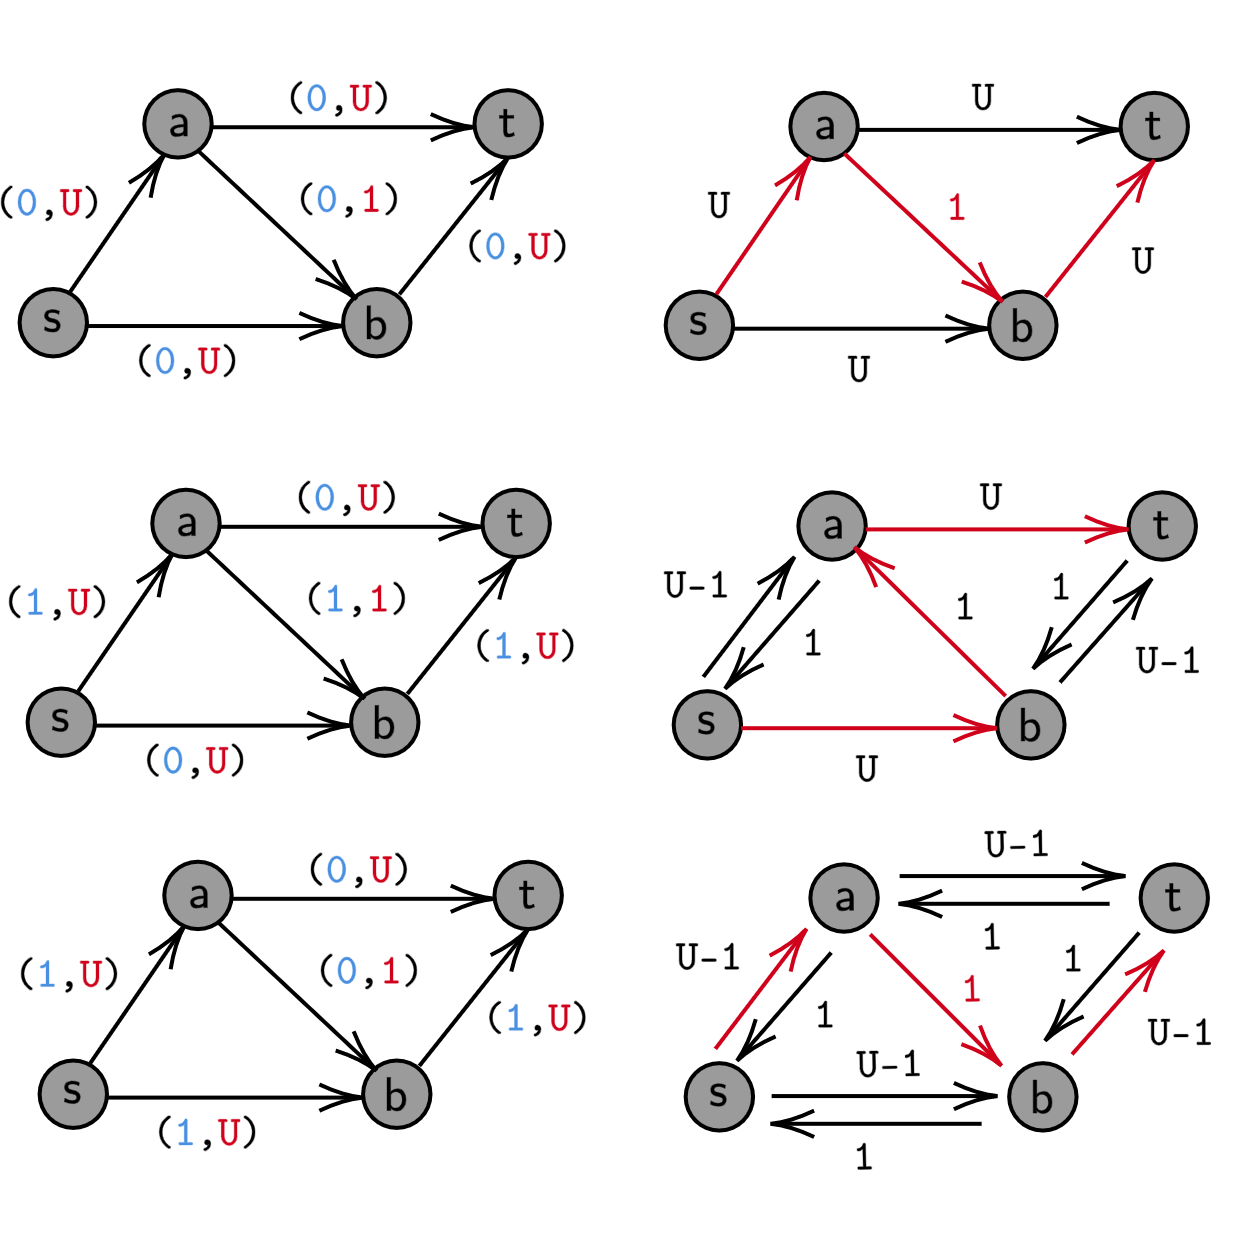
\includegraphics[width=\textwidth]{title.png}

        \vspace{1pc}%
				% \fontsize{10}{12}\selectfont\par\noindent{\textbf{Figure 1.} Example of the \texttt{Ford-Fulkerson} algorithm.}
        \vspace{12pc}%
        \vfill
        % \fontsize{14}{16}\selectfont\par\noindent\thanklesspublisher%

        \end{fullwidth}%
    }%
    \thispagestyle{empty}%
    \clearpage
}
\makeatother

\begin{document}
\maketitlepage
\tableofcontents
\newpage

\section{Network Flow}
  	\subsection{Maximum Flow Problem}
	\begin{defn}[Directed Graph]
		A \textbf{directed graph} is an ordered pair with a set of vertices $V(G)$ and an arc set $A(G) \subseteq \binom{V}{2}$ containing directed edges.
	\end{defn}

	\begin{marginfigure}
		Let $G = (V,A)$ be a directed graph,
		\begin{itemize}
			\item $|V(G)| = n$
			\item $|A(G)| = m$
		\end{itemize}
	\end{marginfigure}

	\begin{defn}[Directed Path]
		A \textbf{directed path} in a directed graph is a path in which every edge is traversed from tail to head.
	\end{defn}

	\begin{defn}[Directed Neighborhood]
		$\delta^+(X)$ is the set of arcs with a tail in $X$ and a head in $V(G) - X$. In contrast, $\delta^-(X) = \delta^+(V(G)-X)$.
	\end{defn}

	\begin{defn}[Capacity]
		Every arc $a = (i,j)$ in $A(G)$ has an integral\footnote{$u_a > 0$ for all arcs $a \in A(G)$. If an arc does not exist, we can assume that it has capacity zero.} \textbf{capacity} $u_a = u_{ij}$, which is the maximum amount that flows through it.
	\end{defn}

	\begin{defn}[Flow]
		Let $G = (V,A)$ be a directed graph. A \textbf{flow} $f$ from a source $s$ to a sink $t$ is a function $f: A(G) \rightarrow R^+$ that satisfies,
		\begin{itemize}
			\item $0 \leq f_a \leq u_a$ for all $a \in A(G)$
			\item $\sum_{a \in \delta^-(v)} f_a = \sum_{a \in \delta^+(v)} f_a$ for all $v \in V(G) - \{s,t\}$
		\end{itemize}
		\noindent The first condition, capacity constraints, states that the flow on an arc $a \in A(G)$ is non-negative and at most its capacity. The second condition, flow conservation, states that the inflow of a vertex $v \not\in \{s,t\}$ equals its outflow.
	\end{defn}

	\begin{defn}[Flow Value]
		Assume that $\delta^+(t) = \delta^-(s) = \emptyset$. Then the \textbf{value} of a flow $f$ is the quantity of flow that reaches the sink,
		\[|f| = \sum_{a \in \delta^-(t)} f_a = \sum_{a \in \delta^+(s)} f_a\]
	\end{defn}

	\begin{defn}[Maximum Flow]
		Let $G = (V, A)$ be a directed graph. The \textbf{maximum flow problem} is the problem of finding $f^*$, where,
		\[
		  f^* = \max \Set{ \sum_{a \in \delta^-(t)} f_a \ | \begin{array}{l}
		    \sum_{a \in \delta^-(v)} f_a = \sum_{a \in \delta^+(v)} f_a \quad \forall v \in V(G) - \{s,t\} \\
		    0 \leq f_a \leq u_a \quad \forall a \in A(G)
		  \end{array}}
		\]
	\end{defn}

	\begin{defn}[Augmenting Path]
		An $(s-t)$ path $P$ is \textbf{augmenting} if\footnote{\begin{center}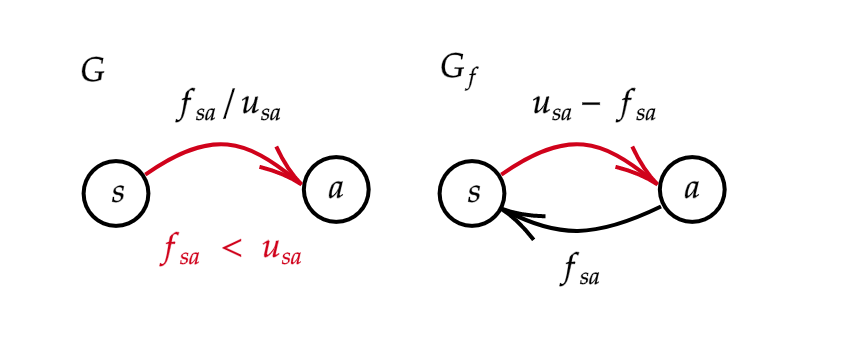
\includegraphics[width=0.5\textwidth]{fig-27.png}\end{center}},
		\begin{itemize}
			\item $f(a) \leq u_a - 1$ for every arc $a$ used in the forward direction of $P$
			\item $f(a) \geq 1$ if $a \in A(P)$ is traversed in the backwards direction
		\end{itemize}
		\noindent Equivalently, $P$ is a directed path from $s$ to $t$ in the residual network $G_f$.
	\end{defn}

	\begin{defn}[Bottleneck Capacity]
		The \textbf{bottleneck capacity} of an augmenting path $P$ with respect to a flow $f$ is the maximum amount $b(P, f)$ that we can increase the flow along $P$ by,
		\[
		b(P, f) = \min \Set{ \min_{\tiny\begin{array}{c} (i,j) \in A \\ i \rightarrow j \end{array}} u_{ij} - f_{ij}, \min_{\tiny\begin{array}{c} (i,j) \in A \\ i \leftarrow j \end{array}} f_{ij}}
		\]
	\end{defn}

	\begin{defn}[Residual Graph]
		Let $G = (V,A)$ be a directed graph, and suppose that $f$ is a flow on $G$. The \textbf{residual graph} $G_f$ satisfies,
		\begin{itemize}
			\item $\exists a_1 \in A(G_f)$ such that $u_{a_1} = u_a - f_a$
			\item $\exists a_2 \in A(G_f)$ such that $u_{a_2} = f_a$
		\end{itemize}
		\noindent for all $a \in A(G)$.
	\end{defn}

	\begin{rmk}
		The bottleneck capacity of a path is the minimum capacity of an arc in the corresponding directed path in the residual graph.
	\end{rmk}

	\begin{defn}[Ford-Fulkerson]
		Let $G = (V,A)$ be a directed graph. The following algorithm produces a maximum flow $f^*$,
	\begin{algorithm}
	  \caption{Ford-Fulkerson}\label{fordfulk}
	  \Comment{$f$ is globally given, and initially set to $0$.}
	  \Function{Augment($P, f$)}{
	  	$b \assign \text{bottleneck capacity $b(P,c)$}$\;
	    \ForEach{$a \in A(P)$}{
	    		\Comment{$|A(P)|$ is at most $|V(G)|$ because $P$ is acyclic.}
		    	\If{$a = (i,j) \text{ is a forward arc}$}{
		    	 \Comment{Increase $f(a)$ in $G$ by $b$.}
		    		$f(a) \assign f(a) + \delta$\;
		      }
		    	\Else{
		    	  \Comment{Decrease $f(a^\prime)$ in $G$ by $b$, where $a^\prime = (j,i)$.}
		     		$f(a^\text{reverse}) \assign f(a^\text{reverse}) + \delta$\;
		     	}
	     	}
	    \Return{$f$}\;
	  }
	  \Function{Ford-Fulkerson($G$)}{
	  	\ForEach{$a \in A(G)$}{
	  		$f(a) \assign 0$\;
	  		$G_f \assign \text{residual network of $G$ with respect to $f$}$;
	  	}
	  	\While{$\exists (s-t) \text{ path $P$ in $G_f$}$}{
	  		$f \assign \FuncCall{Augment}{$P$, $f$}$\;
	  		$\text{Update $G_f$}$;
	  	}
	    \Return{$f$}\;
	  }
	\end{algorithm}
	\end{defn}

	\begin{defn}[Cut]
		$(S, V(G) - S)$ is an \textbf{$(s-t)$ cut} if $s \in S$ and $t \notin S$.
	\end{defn}

	\begin{rmk}
		Let $G = (V, A)$ be a directed graph, and suppose that $f^*$ is the maximum $(s-t)$ flow on $G$. If $S^*$ is the set of vertices that are reachable from $s$ in the residual graph $G_{f^*}$, that is,
		\[S^* = \{v \text{ $|$ } \exists \text{ directed $(s-v)$ path in $G_{f^*}$}\}\]
		\noindent then $(S^*, V(G) - S^*)$ is an $(s-t)$ cut\footnote{Trivially, $s \in S^*$. By the termination condition in \texttt{Ford-Fulkerson}, $t \not\in S^*$. If it was, then there would be an $(s-t)$ path in $G_{f^*}$ and the algorithm would continue for another iteration.} of $G$ and $\delta^+_{G_{f^*}}(S^*) = \emptyset$.
	\end{rmk}

	\begin{ex}{Example of the Cut Lemma}{label}
		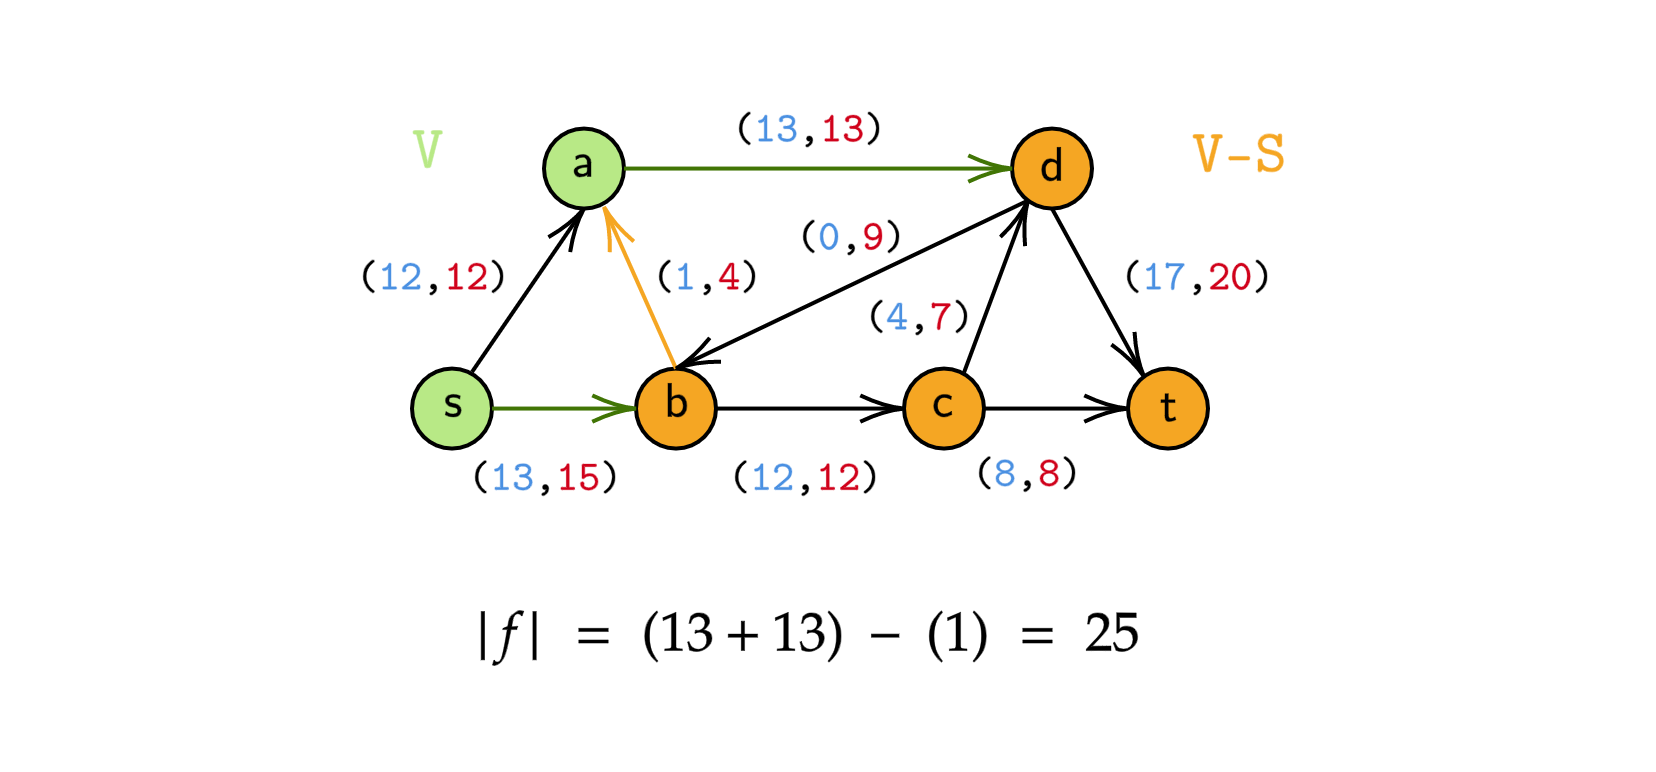
\includegraphics[width=\textwidth]{fig-1.png}
	\end{ex}

	\begin{lem}[Cut Lemma]
		Let $G = (V,A)$ be a directed graph, and suppose that $f$ is an $(s-t)$ flow on $G$. For any $(s-t)$ cut $(S, V - S)$,
		\[|f| = \sum_{a \in \delta^+(S)} f_a - \sum_{a \in \delta^-(S)} f_a\]
	\end{lem}

	\begin{proof}
		The value of $f$ is the amount of flow leaving $s$,
		\begin{align*}
			|f| &= \sum_{a \in \delta^+(s)} f_a \\
					& \text{Since $\delta^-(\{s\}) = \emptyset$,} \\
					&= \sum_{a \in \delta^+(s)} f_a - \sum_{a \in \delta^-(s)} f_a \\
					& \text{By Flow Conservation,} \\
					&= \big(\sum_{a \in \delta^+(s)} f_a - \sum_{a \in \delta^-(s)} f_a \big) + \sum_{v \in S - \{s\}}\big(\sum_{a \in \delta^+(v)} f_a - \sum_{a \in \delta^-(v)} f_a\big) \\
					& \text{Combining the terms to include $s$,} \\
					&= \sum_{v \in S} \big( \sum_{a \in \delta^+(v)} f_a - \sum_{a \in \delta^-(v)} f_a \big) \\
					& \text{Let $a = (i,j) \in A$. There are four cases,}\\
					& \quad \text{1. $(i,j) \in \delta^+(S) \implies f_a$ appears once with coefficient $+1$.} \\ 
					& \quad \text{2. $(i,j) \in \delta^-(S) \implies f_a$ appears once with coefficient $-1$.} \\ 
					& \quad \text{3. $(i,j) \not\in S \implies f_a$ does not appear in the sum.} \\ 
					& \quad \text{4. $(i,j) \in S \implies f_a$ appears twice with coefficients $+1, -1$.} \\ 
					& \text{Consequently,} \\
					&= \sum_{a \in \delta^+(S)} f_a - \sum_{a \in \delta^-(S)} f_a
		\end{align*}
	\end{proof}
		
	\begin{defn}[Cut Capacity]
		\textbf{Capacity} of an $(s-t)$ cut $(S, V - S)$ is,
		\[cap(S) = \sum_{a \in \delta^+(S)} u_a\]
	\end{defn}

	\begin{lem}
		Let $G = (V,A)$ be a directed graph, and suppose that $f$ is an $(s-t)$ flow on $G$. $|f| \leq cap(S)$ for any $(s-t)$ cut $(S, V - S)$.
	\label{lem-ref-1}
	\end{lem}

	\begin{proof}
		By the Cut Lemma,
		\begin{align*}
			|f| &= \sum_{a \in \delta^+(S)} f_a - \sum_{a \in \delta^-(S)} f_a \\
			    &\leq \sum_{a \in \delta^+(S)} f_a \\
			    &= cap(S)
		\end{align*}
	\end{proof}

	\begin{thm}[Maxflow-Mincut]{}
		The maximum value of an $(s-t)$ flow is equal to the minimum capacity of an $(s-t)$ cut.
	\end{thm}

	\begin{proof}
		Let $f^*$ be the flow output by \texttt{Ford-Fulkerson}. Recall that,
		\[S^* = \{v \text{ $|$ } \exists \text{ directed $(s-v)$ path in $G_{f^*}$}\}\]
		\noindent We showed in Lemma \ref{lem-ref-1} that $|f^*| \leq cap(S^*)$, but we can show that $|f^*| = cap(S^*)$. We saw that $\delta^+_{G_{f^*}}(S^*) = \emptyset$ because we could otherwise grow $S^*$. Now, any arc $a \in \delta^+(S^*)$ is not in the residual graph because \texttt{Ford-Fulkerson} requires it to have reached its capacity: $f^*_a = u_a$. Similarly, the reverse of any arc $a \in \delta^-(S^*)$ is not in the residual graph because \texttt{Ford-Fulkerson} requires that $f^*_a = 0$. Now,
		
		\begin{align*}
			|f^*| &= \sum_{a \in \delta^+(S^*)} f_a - \sum_{a \in \delta^-(S^*)} f_a \quad \text{ by the Cut Lemma} \\
			      &= \sum_{a \in \delta^+(S^*)} u_a - \sum_{a \in \delta^-(S^*)} f_a \quad \text{ by Observation 1 above} \\
			      &= \sum_{a \in \delta^+(S^*)} u_a - \sum_{a \in \delta^-(S^*)} 0 \quad \text{ by Observation 2 above} \\
			      &= cap(S^*)
		\end{align*}
	\end{proof}

	\begin{marginfigure}
		$f$ "saturates" the edge $e$ if $f(e) = c(e)$, i.e., $f$ maximizes the flow on $e$. Moreover, if $e$ is not saturated in some maximum $(s-t)$ flow, then $e$ does not occur in any min cut.
		\begin{center}
			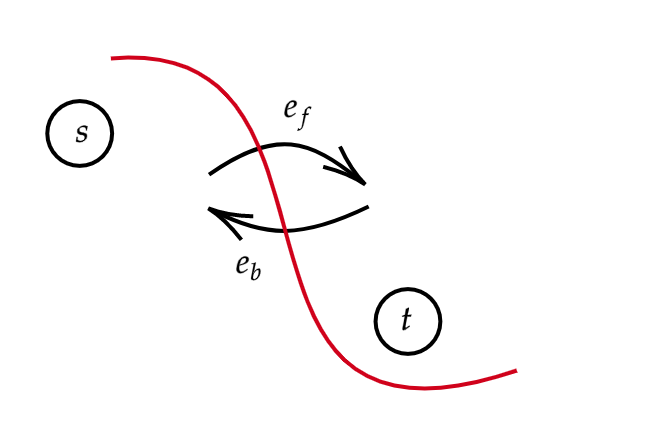
\includegraphics[width=\textwidth]{fig-26.png}
		\end{center}
	\end{marginfigure}

	\begin{rmk}[Running Time]
		\texttt{Ford-Fulkerson} (see Algorithm \ref{fordfulk}) runs in \textbf{pseudo-polynomial time}. Its running time is polynomial in the numeric value of the input, but not in the number of bits required to represent it.
	\end{rmk}

	\begin{proof}
		A single iteration of \texttt{Ford-Fulkerson} runs in $O(m)$ because $G_f$ can be found in $O(m)$, an $(s-t)$ path $P$ can be found in $O(m)$ with Breadth-First Search, and \texttt{Augment} runs in $O(n)$.

		However, the number of iterations is at most $n \cdot U$, where $U$ can be exponential in the input size. The algorithm terminates when $b(P, f) = 0$ for every $(s-t)$ path $P$. Since arc capacities are integral, $b(P,f) \geq 1$. This means that in the worst case, flow is increased by 1 at every iteration. Consequently, the minimum value of any $(s-t)$ cut $C$ satisfies $C \leq n \cdot \max_{a \in A(G)} u_a$. The bound is in terms of $n$, not $m$, because an $(s-t)$ cut separates $V(G)$. Since the flow is at most $n \cdot U$, the number of iterations is bounded by $n \cdot U$.
	\end{proof}

	\begin{ex}{Ford-Fulkerson Running Time Analysis}{label}
		\texttt{Ford-Fulkerson} can take $2U$ iterations on this example,
		\begin{center}
		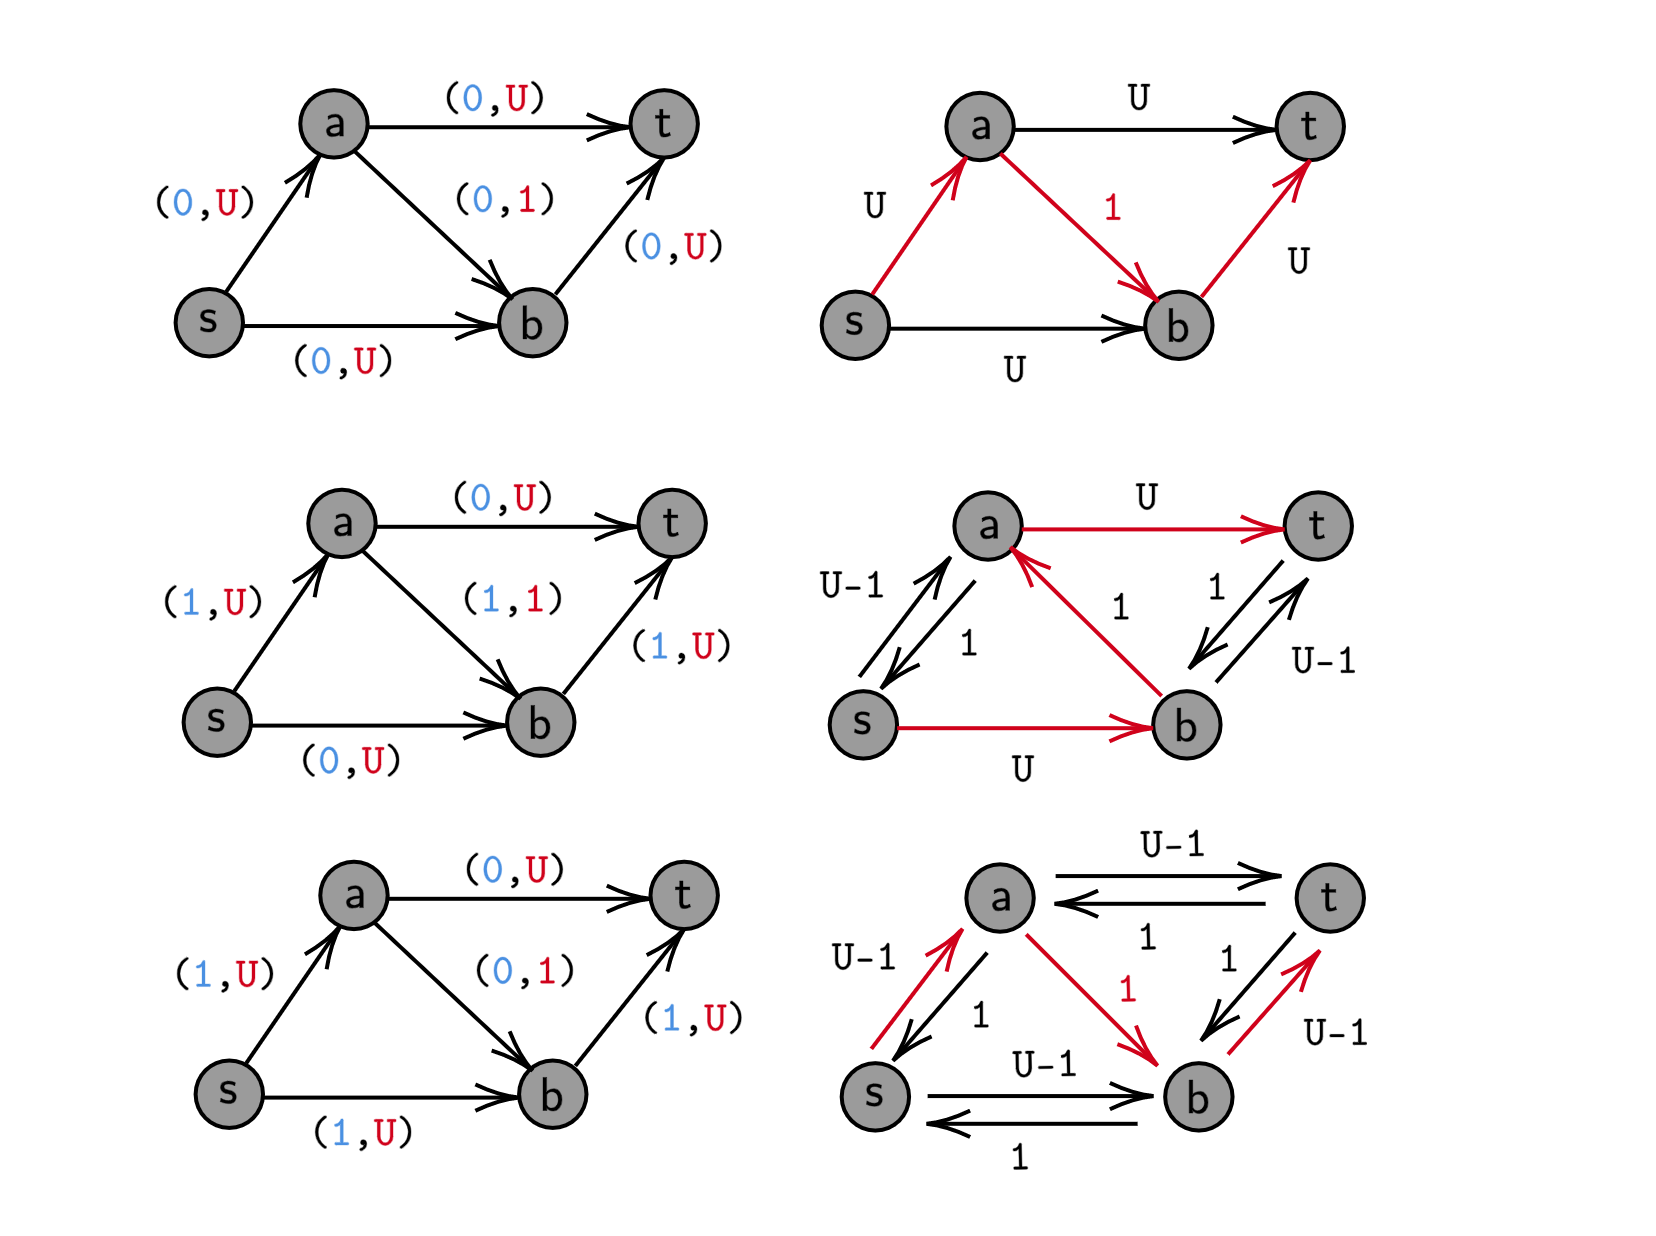
\includegraphics[width=\textwidth]{fig-2.png}
		\end{center}
	\end{ex}

	\subsection{Bipartite Matching Problem}
	\begin{defn}[Independent Set]
 		An \textbf{independent set} is a set of pairwise non-adjacent vertices. The independence number $\alpha(G)$ is the maximal size of an independent set in $G$.
	\end{defn}

	\begin{defn}[Vertex Cover]
 		A \textbf{vertex cover} $X \subset V(G)$ is a set so that every edge of $G$ has an end in $X$. The vertex cover number $\tau(G)$ is the minimum size of a vertex cover in $G$.
	\end{defn}

	\begin{defn}[Matching]
		A \textbf{matching} $M \subset E(G)$ is a set so that every vertex of $G$ is incident to at most one edge of $M$. The matching number $\nu(G)$ is the maximum size of a matching in $G$.
	\end{defn}

	\begin{defn}[Perfect Matching]
		A \textbf{perfect matching} covers $V(G)$.
	\end{defn}

	\begin{defn}[Bipartition]
		A \textbf{bipartition} of a graph $G$ is a pair of subsets $(A, B)$ of $V(G)$ so that $A \cap B = \emptyset$, $A \cup B = V(G)$, and every edge of $G$ has one end in $A$ and another in $B$.
	\end{defn}

	\begin{defn}[Bipartite Matching]
		Let $G = (V, E)$ be an undirected bipartite graph. The \textbf{bipartite matching problem} is the problem of finding $\nu(G)$, the maximum cardinality matching in $G$.
	\end{defn}
 
 	The Ford-Fulkerson Algorithm can be used to solve the bipartite matching problem. To see this, construct an auxiliary network $G = (V, E)$ with bipartition $(X, Y)$ by doing the following,
 	\begin{enumerate}
 		\item Direct each edge $(x_i, y_i)$ from $x_i \rightarrow y_i$
			\item Add a source vertex $s$ with an outgoing arc to each vertex in $X$
			\item Add a sink vertex $t$ with an incoming arc from each vertex in $Y$
			\item Give internal and external arcs capacities of $\infty$ and $1$, respectively\footnote{This is the same as giving every arc a capacity of 1 because the unique arc into each $X$-vertex still has capacity 1}
 	\end{enumerate}

	\begin{ex}{Constructing the Auxiliary Network}{label}
		The auxiliary network for the following bipartite graph is,
		\begin{center}
		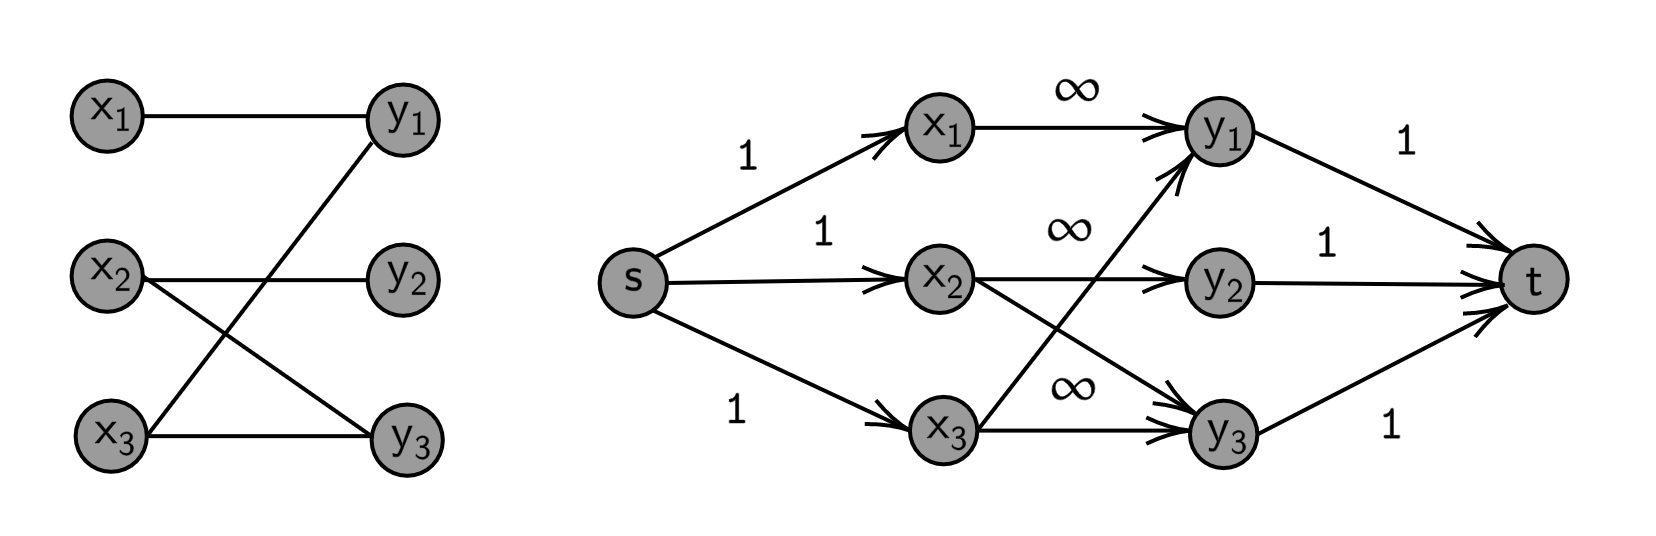
\includegraphics[width=\textwidth]{fig-3.png}
		\end{center}
	\end{ex}

	\begin{thm}[Ford-Fulkerson for Matching]
		There is a polynomial time algorithm to find a maximum cardinality matching in a bipartite graph.
	\end{thm}

	\begin{proof}
		A maximum flow on the auxiliary network is a maximum matching in the original graph. This is because a flow of value $k$ in the auxiliary network consists of $k$ arc-disjoint\footnote{Each arc has capacity 1.} paths, each of which gives an edge in a matching in $G$. Now, since the maximum cardinality of a matching is $\max \{|X|,|Y|\} \leq \frac{n}{2}$, the number of iterations required to run \texttt{Ford-Fulkerson} is at most $n$.
	\end{proof}

	\begin{lem}
		Let $S^*$ be a minimum capacity cut in the auxiliary network of an undirected graph $G$. Every arc in $\delta^+(S^*)$ is of the form $(s, x_i)$ or $(y_j, t)$.
	\end{lem}

	\begin{proof}
		Suppose not. Then $\delta^+(S^*)$ would contain an infinite capacity arc, and so the minimum capacity of a cut in $G$ would be infinite. But the maximum value of a flow on the auxiliary network is $n$ since $s$ has $n$ outgoing arcs, a contradiction.
	\end{proof}

	\begin{thm}[Bipartite Vertex Cover]
		If a vertex cover $C$ and a matching $M$ in a bipartite graph $G$ have the same cardinality, then they are optimal,
		\begin{itemize}
			\item $C$ is a minimum vertex cover
			\item $M$ is a maximum matching
		\end{itemize}
 	\end{thm}

 	\begin{proof}
 		Let $X^* = X \cap S^*$. Then $N(X^*) \subseteq S^* \cap Y$. Otherwise,
 		\[ cap(S^*) = \sum_{a \in \delta^+(S^*)} u_a = \infty \]
 		\noindent $X^* \cup N(X^*) \cup (X - X^*) \cup (N(X - X^*))$ is a partition of $V(G)$. This means that there are three types of edges in $G$,
 		\begin{itemize}
 			\item Edges from $X^*$ to $N(X^*)$
 			\item Edges from $X - X^*$ to $N(X^*)$
 			\item Edges from $X - X^*$ to $Y - N(X^*)$
 		\end{itemize}
 		\noindent We saw above that the fourth type of edge, $X - X^*$ to $N(X^*)$ cannot occur. But then $X - X^* \cup N(X^*)$ is a vertex cover and its cardinality is the capacity of the $(s-t)$ cut.
 	\end{proof}

 	\begin{cor}
 		There is a polynomial time algorithm to find a minimum cardinality vertex cover in a bipartite graph.
 	\end{cor}

 	\subsection{Extensions to Maximum Flow}
 		\begin{defn}[Circulations with Demands]
 		Let $G = (V, A)$ be a directed graph. We associate a demand $d_v$ for flow with each node\footnote{If $d_v < 0$, this indicates that $v$ has supply of $-d_v$. If $d_v = 0$, then the node is neither a source nor a sink.},
 		\begin{itemize}
 			\item $S = \{s_1, \dots, s_k\}$ is the set of sink nodes with positive demand
 			\item $T = \{t_1, \dots, t_l\}$ is the set of source nodes with negative demand
 			\item $s$ is a super-source with arcs $(s,s_i)$ and capacities $d_{s_i}$ for all $s_i \in S$
 			\item $t$ is a super-sink with arcs $(t_j, t)$ and capacities $-d_{t_j}$ for all $t_j \in T$
 		\end{itemize}
 		\noindent A \textbf{circulation with demands} $f: A(G) \rightarrow \{0\} \cup \mathbb{R}^+$ satisfies,
 		\begin{itemize}
 			\item $0 \leq f_a \leq u_a$ for all $a \in A(G)$
 			\item $\sum_{a \in \delta^-(v)} f_a - \sum_{a \in \delta^+(v)} f_a = d_v$ for all $v \in V(G) - \{s,t\}$
 		\end{itemize}
 		\noindent There exists a feasible circulation to the multi-source supply and demand problem if and only if there is a flow from $s$ to $t$ of value $\sum_{v:d_v > 0} d_v = 0$.
 	\end{defn}

	\begin{defn}[Circulations with Demands and Lower Bounds]
 		Let $G = (V, A)$ be a directed graph. We associate a lower bound $l_a = l_{ij}$ on each arc $a = (i,j)$, where $0 \leq l_a \leq u_a$. A \textbf{circulation with demands and lower bounds} can be reduced to one without lower bounds,
 		\begin{itemize}
 			\item $l_e \leq f_a \leq u_a \iff 0 \leq f_a \leq u_a - l_a$ for all $a \in A(G)$
 			\item $d_v^* = d_v + \sum_{(k,v) \in A} l_{kv} - \sum_{(v,k) \in A} l_{vk}$ for all $v \in V(G)$
 		\end{itemize}
 	\end{defn}

 	 	\begin{ex}{Airline Scheduling}{label}
 	 	\begin{tabular}{ll}
			\textbf{\texttt{Origin and Destination}} & \textbf{\texttt{Time}} \\
			\texttt{Boston - San Francisco} & \texttt{7am - 9am} \\
			\texttt{Toronto - Boston} & \texttt{7am - 8am}
		\end{tabular}

		\vphantom{.}

 		We create a network flow as follows,
 		\begin{itemize}
 			\item $o_i$ is a vertex representing the origin of flight $i$
 			\item $d_i$ is a vertex representing the destination of flight $i$
 			\item $s$ is a source vertex with supply $k$
 			\item $t$ is a sink vertex with demand $k$
 			\item $(d_i, t)$ has capacity 1 for every flight $i$
 			\item $(d_i, o_j)$ has capacity 1 if flight $i$ can be serviced after flight $j$
 			\item $(o_i, d_i)$ has a lower bound of 1
 		\end{itemize}
 		There is a way to perform all flights using at most $k$ planes $\iff$ There is a feasible circulation in our network.
	\end{ex}

	\begin{ex}{Open-Pit Mining}{label}
		We are given that,
		\begin{itemize}
			\item $V$ is a set of blocks, each of which generates a profit $\pi_i$
			\item 3 upper neighbors must be removed to dig block $i$
		\end{itemize}
		\noindent We create a network flow as follows,
		\begin{itemize}
			\item $v_i \in V$ represents block $i$ in our pit
			\item $s$ and $t$ are the source and sink vertices
			\item $(s,v_i)$ has capacity $\pi_i$ if and only if $\pi_i > 0$
			\item $(v_i, t)$ has capacity $|\pi_i|$ if and only if $\pi_i < 0$
			\item Infinite capacity arcs exist between $i$ and its 3 neighbors
		\end{itemize}

		We know that $cap(S^*)$ is finite because,
		\[cap(\{s\})= \sum_{i:\pi_i > 0} \pi_i\]
		is finite by construction. The capacity of the an $(s-t)$ cut $S$ is,
		\begin{align*}
			cap(S) &= \sum_{a \in \delta^+(S)}  u_a \\
			       &= \sum_{i \not\in S: \pi_i > 0} \pi_i + \sum_{i \in S: \pi_i > 0} |\pi_i| \\
			       &= \bigg(\sum_{i \in V: \pi_i > 0} \pi_i - \sum_{i \in S: \pi_i > 0} \pi_i \bigg) + \sum_{i \in S: \pi_i > 0} |\pi_i| \\
			       &= \bigg(\sum_{i \in V: \pi_i > 0} \pi_i - \sum_{i \in S: \pi_i > 0} \pi_i \bigg) - \sum_{i \in S: \pi_i > 0} \pi_i \\
			       &= \underbrace{\sum_{i \in V: \pi_i > 0} \pi_i}_{constant} - \sum_{i \in S} \pi_i
		\end{align*}
		Minimizing $cap(S)$ solves the open-pit mining problem, since it requires us to maximize the profit associated with $S$.
	\label{mining}
	\end{ex}

	\begin{ex}{Image Segmentation}{label} 
 		We create a network flow as follows,	
 		\begin{itemize}
 				\item $v_i$ is a vertex representing the pixel $i$
 				\item $s$ is a source vertex representing the foreground
 				\item $t$ is a sink vertex representing the background
 				\item $f_i$ is the likelihood that the pixel $i$ is in the foreground
 				\item $b_i$ is the likelihood that the pixel $i$ is in the background
 				\item $\rho_{ij}$ is a penalty for separating adjacent pixels $i$ and $j$
 				\item $(s, v_i)$ has capacity $f_i$
 				\item $(v_j, t)$ has capacity $b_j$
 				\item $(v_i,v_j)$ and $(v_j,v_i)$ have capacity $\rho_{ij}$
 		\end{itemize}

 		The capacity of the an $(s-t)$ cut $S$ is,
 		\begin{align*}
 			cap(S) &= \sum_{a \in \delta^+(S)}  u_a \\
 			       &= \sum_{i \not\in S} f_i + \sum_{j \in S} b_j + \sum_{(i,j) \in \delta^+(S)} \rho_{ij} \\
 			       &= \big(\sum_{i \in V} f_i - \sum_{i \in S} f_i\big) + \big(\sum_{j \in V} b_j - \sum_{j \not\in S} b_j\big) + \sum_{(i,j) \in \delta^+(S)} \rho_{ij} \\
 			       &= \underbrace{\sum_{i \in V}(f_i + b_i)}_{constant} - \sum_{i \in S}f_i - \sum_{j \not\in S}b_j + \sum_{(i,j) \in \delta^+(S)} \rho_{ij}
 		\end{align*}

 		Minimizing $cap(S)$ is solves the segmentation problem,
 		\[ \max_S \sum_{i \in S}f_i + \sum_{j \not\in S} b_j - \sum_{(i,j) \in \delta^+(S)} \rho_{ij}\]
 		\begin{itemize}
 			\item There is a bonus $f_i$ if pixel $i$ is placed in the foreground
 			\item There is a bonus $b_j$ if pixel $j$ is placed in the background
 			\item There is a penalty $\rho_{ij}$ for separating pixels $i$ and $j$
 		\end{itemize}
 	\end{ex}

 	\subsection{Flow Decomposition Theorem}
 	\begin{marginfigure}
	\textbf{Recap on Flow Decomposition:}

	\noindent Let $G = (V, A)$ be a directed graph and suppose that $f$ is an $(s-t)$ flow of value $k$. Then there exist directed paths $P_1, \dots, P_k$ (possibly repeated) from $s$ to $t$ in $G$, and every edge belongs to at most $f(e)$ paths.
	\end{marginfigure}

	\begin{lem}
		Let $G = (V, A)$ be a directed graph and suppose that $f$ is an $(s-t)$ flow of value $k > 0$ Then $f$ contains a path or a cycle.
	\label{fdtlemma}
	\end{lem}

	\begin{proof}
		If $f$ contains a directed cycle $C$, then we are done. Assume that this is not the case. Since $k > 0$,
		\[ \sum_{a \in \delta^+(\{s\})}f_a \geq 1\]
		\noindent so there is at least one arc $a_1 = (s, v_1)$ with $f_{a_1} \geq 1$. By flow conservation, there exists an arc $a_2 = (v_1, v_2)$ ($v_2 \neq s$ since the flow is acyclic). Repeating inductively, we can construct an $(s-t)$ path with $\min_{a \in P}f_a \geq 1$.
	\end{proof}

	\begin{thm}[Flow Decomposition Theorem]
		Let $G = (V, A)$ be a directed graph and suppose that $f$ is an $(s-t)$ flow of value $k > 0$. Then $f$ can be decomposed into at most $m$ $(s-t)$ paths and directed cycles.
	\end{thm}

	\begin{proof}
		We proceed by induction on the number of arcs in the graph.
		\begin{itemize}
			\item (Base Case) If $m = 0$, then $f$ is empty and trivially consists of zero paths and cycles. If $m = 1$, then $f$ is a single arc $(s,t)$ and thus can be decomposed into one $(s,t)$ path.
			\item (Induction Hypothesis) Assume that any flow with $k < m$ arcs can be decomposed into a collection of at most $k$ cycles and $(s-t)$ paths. Consider a flow $f$ with $m$ arcs. By Lemma \ref{fdtlemma}, $f$ contains a path or a cycle. There are two cases,
			\begin{enumerate}
				\item If $f$ contains a cycle $C$, then let $f^*$ be the flow obtained by removing $\min_{a \in C}f_a$ units of flow from each arc in $C$. Then $f^*$ has at least one fewer arc than $f$. By the induction hypothesis, $f^*$ decomposes into at most $m-1$ paths and cycles. Thus, $f$ decomposes into at most $m$ paths and cycles.
				\item If $f$ contains a path $P$, then let $f^*$ be the flow obtained by removing $\min_{a \in C}f_a$ units of flow from each arc in $P$. Proceed as in Case 1 to decompose $f^*$ into $m-1$ paths and cycles.
			\end{enumerate}
		\end{itemize}		
	\end{proof}

	\begin{cor}
		The Ford-Fulkerson algorithm can terminate in $m$ iterations.
	\end{cor}

	\subsection{Fast Flow Algorithms}
	\begin{rmk}
		Let $G = (V, A)$ be a directed graph and suppose that $f^*$ is an maximum $(s-t)$ flow on $G$. Then there is a path $P$ in $G$ with,
		\[u_P \geq \frac{1}{m}|f^*|\]
	\end{rmk}

	\begin{proof}
		By the Flow Decomposition Theorem, $f^*$ consists of at most $m$ paths. Thus, at least one of these paths carries $\frac{1}{m}|f^*|$ flow.
	\end{proof}

	\begin{rmk}
		Let $G = (V, A)$ be a directed graph and suppose that $f^*$ is an maximum $(s-t)$ flow on $G$. Let $f$ be any other $(s-t)$ flow on $G$. Then,
		\[b(P, f) \geq \frac{|f^*|-|f|}{m}\]
		\noindent for some path in the residual graph $G_f$.
		\label{observ1}
	\end{rmk}

	\begin{proof}
		$f^* - f$ satisfies the flow conservation constraints. By the Flow Decomposition Theorem, $f^* - f$ can be decomposed into at most $2m$ paths and cycles. Only one direction of each arc is used, so we can assume that $(f^*-f)$ can be decomposed into at most $m$ paths. Thus, at least one of these paths carries $\frac{|f^*|-|f|}{m}$.
	\end{proof}

	\begin{defn}[Maximum Capacity]
		The \textbf{maximum capacity augmenting path algorithm} chooses augmenting paths greedily by capacity.
	\end{defn}

	\begin{marginfigure}
		\textbf{(Recap)} $1 - x < e^{-x}$ for all $x \neq 0$.
	\end{marginfigure}
	
	\begin{thm}
		The maximum capacity augmenting path algorithm terminates in at most $m \cdot (\ln n + \ln U)$ iterations\footnote{Weakly polynomial algorithms depend on the size of the input.}, where $U = \max_{a \in A}u_a$.
	\end{thm}

	\begin{proof}
		Suppose that the algorithm finds paths $\{P_1, P_2, \dots, P_T\}$. We need to show that $T \leq m \cdot (\ln n + \ln U)$. Denote by $f_t$ the flow after $t$ iterations. By Remark \ref{observ1}, the path $P_{t+1}$ satisfies,
		\[b(P_{t+1}, f_t) \geq \frac{|f^*|-|f_t|}{m} := \frac{\triangle_{t+1}}{m}\]
		\noindent $\triangle_{t+1}$ is the flow quantity that remains to be found at step $t+1$. In particular, $\triangle_{t+1} \leq \triangle_t - \frac{1}{m}\cdot \triangle_t$ since we fall by $\frac{1}{m}$ at each iteration. Continuing inductively, we get that $\triangle_{t+1} \leq (1 - \frac{1}{m})^t \cdot \triangle_1 = (1 - \frac{1}{m})^t \cdot |f^*|$. But then, $\triangle_{t+1} \leq e^{-\frac{t}{m}} \cdot |f^*|$. Setting $t = m \cdot ln|f^*|$,
		\[\triangle_{t+1} < e^{-\frac{m \cdot ln|f^*|}{m}} |f^*| = 1\]
		\noindent After $T=m \cdot \ln|f^*|$ steps, the quantity of flow remaining to be found is less than one. Flows are integral, so we have found $|f^*|$. Since the maximum cut in $G$ has value $n\cdot U$, $\ln|f^*| \leq \ln u \cdot U = \ln u + \ln U$. Thus, the number of iterations is at most $m \cdot (\ln u + \ln U)$.
	\end{proof}

	\begin{algorithm}
	  \caption{Maximum Capacity Augmenting Paths}\label{greedyaug}
	  \Comment{$f$ is globally given, and initially set to $0$.}
	  \Comment{$\texttt{Augment}(P,f)$ is globally given}
	  \Function{Ford-Fulkerson($G$)}{
	  	\ForEach{$a \in A(G)$}{
	  		$f(a) \assign 0$\;
	  		$G_f \assign \text{residual network of $G$ with respect to $f$}$;
	  	}
	  	\While{$\exists (s-t) \text{ path $P$ in $G_f$}$}{
	  		$P^* \assign \text{maximum capacity augmenting path}$
	  		$f \assign \FuncCall{Augment}{$P^*$, $f$}$\;
	  		$\text{Update $G_f$}$;
	  	}
	    \Return{$f$}\;
	  }
	\end{algorithm}

	\begin{thm}
		The maximum capacity augmenting path algorithm takes $O(m^2)$ time per iteration. Binary search reduces it to $O(m \cdot \log m)$.
	\end{thm}

	\begin{proof}
		Label the arcs in $G_f$ by \{1, 2, \dots, 2m\} in decreasing order of residual capacity. We can test if there is an $(s-t)$ path that uses arcs $\{1, \dots k\}$ in $O(m)$ time by Breadth-First Search. Repeating this process for all $k$ gives a total time in $O(m^2)$.
	\end{proof}

	\begin{cor}
		It total, the algorithm runs in $O(m^3 \cdot (\ln u + \ln U))$ time.
	\end{cor}

	\begin{defn}[Shortest Length]
		The \textbf{shortest length residual path algorithm} chooses augmenting path greedily by length\footnote{The length of a path is the number of arcs comprising it.}.
	\end{defn}

	\begin{marginfigure}
		\textbf{The Potential Function Argument:}

		If $\phi$ satisfies,
		\begin{itemize}
			\item $\phi$ decreases at a rate of $\delta$
			\item $\phi$ is lower bounded by $\ell$
		\end{itemize}
		\noindent Then $\phi$ becomes fixed at time $T$. Given the starting value $\phi_0$ and $\ell$, we know that $\phi$ becomes fixed at $-\phi_0*|\delta| = \phi$.
	\end{marginfigure}

	\begin{rmk}
		An iteration of the shortest length augmenting path algorithm is in $O(m)$ if the shortest $(s-t)$ paths are found with Breadth-First Search.
	\end{rmk}

	\begin{thm}
		The shortest length augmenting path algorithm terminates in at most $m \cdot n$ iterations. This puts its runtime in $O(m^2 \cdot n)$.
	\end{thm}

	\begin{proof}
		Suppose that the algorithm finds paths $\{P_1, P_2, \dots, P_T\}$. We need to show that $T \leq m \cdot n$. Let $f_t$ be the flow after $t$ iterations, and consider its residual graph $G_{f_t}$. Define $d_t(v)$ as the distance of a vertex $v$ from the source $s$ in $G_{f_t}$, and consider $\phi_t = \sum_{v \in V} d_t(v)$. We will use a potential energy function argument to show that,
		\[d_t(u) \leq d_{t+1}(u) \quad \text{for all $t$}\]
		
		\noindent If $t = 0$, then $\phi_0 = \sum_{v \in V} d_0(v) \geq 0$ since $d_0$ is a distance. Moreover, $d_t(v) \leq n - 1$ since $G$ has $n$ vertices. This means that,
		\[\phi_t = \sum_{v \in V}d_t(v) \leq n^2\]

		\noindent To apply the argument, we need to prove that $\phi_t$ is non-decreasing. It suffices to show that $d_t(v)$ is non-decreasing for each vertex $v$. Suppose not. Then there exists $t \in \mathbb{N}$ and a vertex $v \in V(G)$ such that $d_t(v) > d_{t+1}(v)$. Consider the closest such vertex to $s$. Let $u$ be the vertex preceding it on the shortest path from $s$ to $v$ in $G_{f_{t+1}}$. Then $d_{t+1}(v) = d_{t+1}(u) + 1$ and $d_t(u) \leq d_{t+1}(u)$.
		\begin{itemize}
			\item If $(u,v) \in G_{f_t}$, then,	
			\begin{align*}
				d_t(v) &\leq d_t(u) + 1 \text{\phantom{ since $P_t$ is the shortest path in $G_{f_t}$}}\\
							 &\leq d_{t+1}(u) + 1 \text{ since $d_t(u) \leq d_{t+1}(u)$} \\
							 &= d_{t+1}(v) \text{ since $d_{t+1}(v) = d_{t+1}(u)+1$} \\
							 &< d_{t+1}(v) \text{ since $d_t(v) > d_{t+1}(v)$} \\
							 &\text{a contradiction.}
			\end{align*}
			\item If $(u,v) \not\in G_{f_t}$, $(v,u) \in P_t$ since $(u,v) \in G_{f_{t+1}}$. But,
			\begin{align*}
				d_t(u) &= d_t(v) + 1 \text{ since $P_t$ is the shortest path in $G_{f_t}$} \\
						   &> d_{t+1}(v) + 1 \\ 
						   &= d_{t+1}(u) + 2 \text{ since $d_{t+1}(v) = d_{t+1}(u)+1$} \\
						   &\geq d_t(u) + 2 \\
						   &\text{a contradiction.}
			\end{align*}
		\end{itemize}

		\noindent $P_t$ is augmented by its bottleneck capacity, and there is at least one arc $a_t$ with that capacity. It suffices to prove that each arc can be the bottleneck arc at most $\frac{n}{2}$ times\footnote{This argument works because we have proven that $\phi$ is a bounded function.}, because this means that the number of iterations is at most $2m \cdot \frac{n}{2} = mn$.
	\end{proof}

	\begin{lem}
		Each arc can be the bottleneck arc at most $\frac{n}{2}$ times.
	\end{lem}

	\begin{proof}
		Let $(u,v) \in A(G_{f_t})$ be the bottleneck arc in the augmenting path $P_t$. Since $P_t$ is the shortest $(s-t)$ path in $G_{f_t}$, we have that $d_t(v) = d_t(u) + 1$. Now, $(u,v) \not\in G_{f_{t+1}}$ since $(u,v)$ is the bottleneck arc in iteration $t$. Suppose that $(u,v)$ is a bottleneck in iteration\footnote{$(u,v)$ cannot be a bottleneck at iteration $t + 1$ because it is not in the residual graph $G_{f_{t+1}}$.} $t + 1 + k > t + 1$ ($k > 0$). Then $(u,v)$ must have been added back into the residual graph $G_{f_{t + 1 + k}}$. This means that the reverse arc $(v,u)$ must have been used at some time $t + 1 \leq t^{\prime} < t + 1 + k$. As $P_{t^{\prime}}$ is the shortest $(s-t)$ path in $G_{f_{t^{\prime}}}$, we have:
		\begin{align*}
			d_{t^{\prime}}(u) &= d_{t^{\prime}}(v) + 1 \\
			&\geq d_t(v) + 1\\
			&= d_t(u) + 2
		\end{align*}
		\noindent Since the distance label of $u$ must have increased by at least 2, this can happen at most $\frac{n}{2}$ times. Otherwise, we get that $d_t(u) > n$.
	\end{proof}

		\begin{algorithm}
	  \caption{Shortest Length Augmenting Paths}\label{greedyaug}
	  \Comment{$f$ is globally given, and initially set to $0$.}
	  \Comment{$\texttt{Augment}(P,f)$ is globally given}
	  \Function{Ford-Fulkerson($G$)}{
	  	\ForEach{$a \in A(G)$}{
	  		$f(a) \assign 0$\;
	  		$G_f \assign \text{residual network of $G$ with respect to $f$}$;
	  	}
	  	\While{$\exists (s-t) \text{ path $P$ in $G_f$}$}{
	  		$P^* \assign \text{shortest length augmenting path}$
	  		$f \assign \FuncCall{Augment}{$P^*$, $f$}$\;
	  		$\text{Update $G_f$}$;
	  	}
	    \Return{$f$}\;
	  }
	\end{algorithm}

\section{Linear Programming}
  \subsection{Formulating Linear Programming Problems}
	\begin{ex}{The Diet Problem}{label}
		A student is subject to the following dietary requirements,

		\vphantom{.}

		\resizebox{\textwidth}{!}{
		\begin{tabular}{llllll}
		\textbf{Food} & \textbf{Energy} & \textbf{Protein} & \textbf{Calcium} & \textbf{Price} & \textbf{Servings} \\ \hline
		Porridge & 110 & 4 & 2 & 10 & 4 \\ \hline
		Chicken & 205 & 32 & 12 & 200 & 3 \\ \hline
		Eggs & 160 & 13 & 54 & 40 & 4 \\ \hline
		Milk & 160 & 8 & 285 & 35 & 8 \\ \hline
		Apple Pie & 420 & 4 & 22 & 190 & 3 \\ \hline
		Pork and Beans & 260 & 14 & 80 & 90 & 2 \\ \hline
		Requirement & 2000 & 55 & 800 & None & None \\
		\end{tabular}}

		\vphantom{.}

		\noindent The goal is to find,
		\[\min 10x_1 + 200x_2 + 40x_3 + 35x_4 + 190x_5 + 90x_6 \]
		\noindent subject to the constraints,
		\begin{align*}
			x_i \geq 0 \text{ for all $i \in [6]$} & \\
			x_1 \leq 4, x_2 \leq 3, x_3 \leq 4, x_4 \leq 8, x_5 \leq 3, x_6 \leq 2 & \\
			110x_1 + 205x_2 + 160x_3 + 160x_4 + 420x_5 + 260x_6 &= 2000 \\
			4x_1 + 32x_2 + 13x_3 + 8x_4 + 4x_5 + 14x_6 &= 55 \\
			2x_1 + 12x_2 + 54x_3 + 285x_4 + 22x_5 + 80x_6 &= 800 \\
		\end{align*}

	\end{ex}

	\begin{marginfigure}
		\begin{center}
			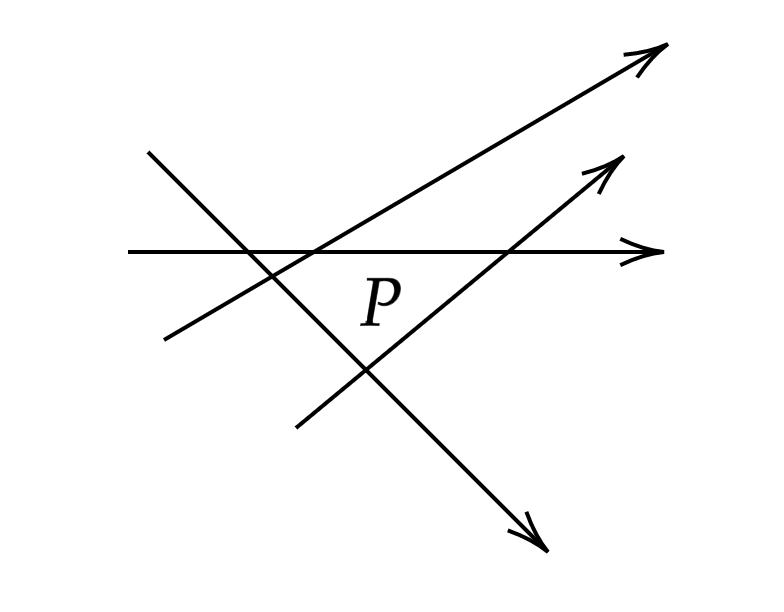
\includegraphics[width=0.6\textwidth]{fig-4.png}
		\end{center}

		\noindent Any linear equation in $n$ variables defines a hyperplane in $\mathbb{R}^n$, and the intersection of a finite number of hyperplanes is called a polyhedron. By rotating the space so that the objective function points downward, any linear program is the problem of finding the lowest point in a given polyhedron.
	\end{marginfigure}

	\begin{defn}[Linear Program]
		A \textbf{linear program} minimizes or maximizes a linear objective function subject to a set of linear constraints.
	\end{defn}

	\begin{defn}[Feasibility]
		A point $x \in \mathbb{R}^n$ is \textbf{feasible} with respect to some linear program if it satisfies all of the linear constraints.
	\end{defn}

	\begin{defn}[Primal Linear Program]
		A primal linear program is,
		\[
		    \max \Set{ \sum_{j=1}^n c_j \cdot x_j \ | \begin{array}{l}
		    \sum_{j=1}^n a_{ij} \cdot x_j \leq b_j \text{ for all } i \in [m] \\
		    x_j \geq 0 \text{ for all } j \in [n]
		  \end{array}}
		\]	
	\end{defn}

	\begin{rmk}
		The matrix encoding of a linear program in standard form is,
		\[
		    \max \Set{ c^T \cdot x \ | \begin{array}{l}
		    Ax \leq b \\
		    x \geq 0
		  \end{array}}
		\]	
	\end{rmk}

	\begin{ex}{Standard Form}{label}
		Any linear program can be converted into standard form,
		\[
		\begin{array}{ll}
		\operatorname{maximise} & \sum_{j=1}^{n} c_{j} x_{j} \\
		\text { subject to } & \sum_{j=1}^{n} a_{i j} x_{j} \leq b_{i} \quad \forall i \in[m] \\
		& x_{j}  \geq 0  \quad \forall j \in[n]
		\end{array}
		\]
		\begin{itemize}
			\item For each variable $x_j$, add:
				\begin{itemize}
					\item Two new variables $x_i^+, x_i^-$
					\item Recover $x_j$ by taking, $x_j = x_j^+ - x_j^-$
					\item Inequalities, $x_j^+ \geq 0$ and $x_j^- \geq 0$
				\end{itemize}
			\item Replace any equality constraint $\sum_j a_{ij}x_j = b_i$ with:
				\begin{itemize}
					\item An inequality constraint, $\sum_j a_{ij}x_j \geq b_i$
					\item An inequality constraint $\sum_j a_{ij}x_j \leq b_i$
				\end{itemize}
			\item Replace any upper bound constraint $\sum_j a_{ij}x_j \geq b_i$ with,
					\begin{itemize}
						\item The equivalent lower bound, $\sum_j -a_{ij}x_j \leq -b_i$
					\end{itemize}
			\end{itemize}
	\end{ex}

		\begin{defn}[Dual Linear Program]
			For every primal linear program,
			\[
			\begin{array}{lrlr}
			\operatorname{maximize} & \sum_{j=1}^{n} c_{j} \cdot x_{j} & & \\
			\text { subject to } & \sum_{j=1}^{n} a_{i j} \cdot x_{j} & \leq b_{i} &\forall i \in[m] \\
			& x_{j} & \geq 0 & \forall j \in[n]
			\end{array}
			\]
			\noindent there is a corresponding \textbf{dual linear program},
			\[
			\begin{array}{lrlr}

			\operatorname{minimize} & \sum_{i=1}^{m} b_{i} \cdot y_{i} & & \\
			\text { subject to } & \sum_{i=1}^{m} a_{i j} \cdot y_{i} & \geq c_{j} & \forall j \in[n] \\
			& y_{i} & \geq 0 & \forall i \in[m]
			\end{array}
			\]
			 that can be obtained by swapping the constraints and the variables.
		\end{defn}

		\begin{rmk}
			The matrix encoding of the dual linear program is,
			\[
		    \min \underbrace{\Set{ b^Ty \ | \begin{array}{l}
		    A^T y \geq c \\
		    y \geq 0
		  \end{array}}}_{Dual}
			\iff
			\max \underbrace{\Set{ c^Tx \ | \begin{array}{l}
		    Ax \leq b \\
		    x \geq 0
		  \end{array}}}_{Primal}
		\]	
		\end{rmk}

	\begin{defn}[Dictionaries]
		Given a linear program in standard form,
		\[
		    \max \Set{ \sum_{j=1}^n c_j \cdot x_j \ | \begin{array}{l}
		    \sum_{j=1}^n a_{ij} \cdot x_j \leq b_j \text{ for all } i \in [m] \\
		    x_j \geq 0 \text{ for all } j \in [n]
		  \end{array}}
		\]	
		\noindent we introduce \textbf{slack variables}\footnote{Slack variables are variables that has been introduced to turn an inequality constraint into an equality constraint.} $x_{n+1}, x_{n+2}, \cdots, x_{n + m}$,
		\[x_{n+i} = b_i - \sum_{j=1}^n a_{ij} \cdot x_j \quad \text{for $i \in [m]$ and } \quad z = \sum_{j=1}^n c_j \cdot x_j \]
		\noindent and denote the objective function by $z$.
	\end{defn}

	\begin{defn}[Basic Variable]
		\textbf{Basic} variables are the variables that appear on the left-hand side of a dictionary, and they constitute a basis.
	\end{defn}

	\begin{defn}[Nonbasic Variable]
		\textbf{Nonbasic} variables are the variables that appear on the right-hand side of a dictionary.
	\end{defn}

	\begin{rmk}
		Dictionaries define basic variables in terms of non-basic ones.
	\end{rmk}

	\subsection{The Simplex Algorithm: Method}
	\begin{defn}[Simplex Algorithm]
		The \textbf{simplex algorithm} works as the Gauss-Jordan elimination method on inequalities and constraints,
		\begin{itemize}
			\item Represent the linear program in slack form
			\item Convert one slack form into an equivalent slack form, ensuring that the value of the objective function does not decrease while likely increasing it
			\item Repeat until the optimal solution becomes apparent
		\end{itemize}
	\end{defn}

	\begin{ex}{Slack Variables}{label}
		Take the linear program, 
		\[
		\begin{array}{cl}
		\operatorname{maximize} & 5 x_{1}+4 x_{2}+3 x_{3} \\
		\text { subject to } & 2 x_{1}+3 x_{2}+x_{3} \leq 5 \\
		& 4 x_{1}+x_{2}+2 x_{3} \leq 11 \\
		& 3 x_{1}+4 x_{2}+2 x_{3} \leq 8 \\
		& x_{1}, x_{2}, x_{3} \geq 0
		\end{array}
		\]
		\noindent Write it in dictionary form,

		\vphantom{.}

		\begin{center}
		\begin{tabular}{lllllllll}
		$z$   & = &    &     & $5x_1$ & $+$ & $4x_2$ & $+$ & $3x_3$ \\ \hline
		$x_4$ & = & 5  & $-$ & $2x_1$ & $-$ & $3x_2$ & $-$ & $x_3$  \\
		$x_5$ & = & 11 & $-$ & $4x_1$ & $-$ & $x_2$  & $-$ & $2x_3$ \\
		$x_6$ & = & 8  & $-$ & $3x_1$ & $-$ & $4x_2$ & $-$ & $2x_3$
		\end{tabular}
		\end{center}

		\vphantom{.}

		\noindent and restate our problem as,
		\[
		\begin{array}{cl}
		\operatorname{maximize} & z \\
		\text { subject to } & x_{1}, x_{2}, x_{3}, x_{4}, x_{5}, x_{6} \geq 0
		\end{array}
		\]
	\end{ex}

	\begin{ex}{The Simplex Algorithm}{label}
	The \textbf{feasible solution} that is implicit in our dictionary is,
	\[(x_1, x_2, x_3, x_4, x_5, x_6) = (0,0,0,5,11,8)\]

	This gives an \textbf{objective value} of,
	\[z = 5x_1 + 4x_2 + 3x_3 = 0\]

	In the first iteration, we attempt to increase the value of $z$ by making one of the right-hand side variables positive.
	\end{ex}

	\begin{marginfigure}
		\textbf{Linear Programming Algorithms:}
		\begin{itemize}
			\item \textit{Simplex Algorithm.} In the feasible region, $x$ moves from vertex to vertex in the direction of $c$. The algorithm is simple, but runs in exponential time in the worst case.
			\item \textit{Ellipsoid Algorithm.} The algorithm begins with an ellipsoid that includes the optimal solution, and continues to shrink the ellipsoid until the optimal solution is found.
			\item \textit{Interior Point Method.} $x$ moves inside the polytope following $c$.
		\end{itemize}
	\end{marginfigure}

	\begin{defn}[Entering Variable]
		The \textbf{entering variable} at each iteration is the nonbasic variable that enters the basis to increase $z$\footnote{We may choose any nonbasic variable with a positive coefficient in the top row of the dictionary.}. 
	\end{defn}

	\begin{defn}[Leaving Variable]
		The \textbf{leaving variable} at each iteration is the variable that is removed from the basis for the entering variable\footnote{We may choose any basic variable whose non-negativity imposes the most stringent upper bound on the increment of the entering variable.}. 
	\end{defn}

	\begin{ex}{The Simplex Algorithm}{label}
		The entering variable in the first iteration is $x_1$. Since $x_1, x_2, x_3$ are all positive, we choose the variable with the largest coefficient in order to increase $z$ at the fastest rate.

		\vphantom{.}
		\begin{center}
		\begin{tabular}{lllllllll}
		$z$   & = & $\frac{25}{2}$ & $-$   & $\frac{7}{2}x_2$  & $+$ & $\frac{1}{2}x_3$  & $-$ & $\frac{5}{2}x_4$ \\ \hline
		$x_1$ & = & $\frac{5}{2}$ & $-$ & $\frac{3}{2}x_2$ & $-$ & $\frac{1}{2}x_3$ & $-$ & $\frac{1}{2}x_4$ \\
		$x_5$ & = & 1 & $+$ & $5x_2$ & & & $+$ & $2x_4$ \\
		$x_6$ & = & $\frac{1}{2}x_2$ & $+$ & $\frac{1}{2}x_3$ & $-$ & $\frac{1}{2}x_3$ & $+$ & $\frac{3}{2}x_4$
		\end{tabular}
		\end{center}
		\vphantom{.}

		This completes the first iteration of the simplex method, and,
		\[(x_1, x_2, x_3, x_4, x_5, x_6) = \bigg(\frac{5}{2},0,0,0,1,\frac{1}{2}\bigg)\]
	\end{ex}

	\subsection{The Simplex Algorithm: Termination}
	\begin{defn}[Cycling]
		The simplex algorithm \textbf{cycles} if one dictionary appears in two or more iterations. Cycling prevents termination.
	\end{defn}

	\begin{defn}[Smallest Subscript Rule]
		The \textbf{smallest-subscript rule} is a rule for breaking ties in the choice of the entering and leaving variables. It always chooses the candidate $x_k$ by the smallest subscript $k$. 
	\end{defn}

	\begin{thm}[Bland's Rule]
		The simplex method terminates as long as the entering and leaving variables are selected by the smallest-subscript rule.
	\end{thm}

	\begin{proof}
		Assume not. Then there exists a sequence of degenerate iterations that produces dictinaries $D_1, D_2, \cdots D_k$ such that $D_k = D_0$. A variable is called \textbf{fickle} if it is nonbasic in some dictionaries, but basic in others. Let $x_t$ be the fickle variable with the largest subscript. Then there is a dictionary $D$ in the sequence $D_0, \cdots, D_k$ such that $x_t$ leaves and some other fickle variable $x_s$ enters. Further along,
		\[\underbrace{D_0}_{=D_k}, D_1, \cdots, D_k, D_1, \cdots, D_k\]
		\noindent there is another dictionary $D^*$ with $x_t$ entering,
		\[\begin{aligned}
		&x_{i}=b_{i}-\sum_{j \notin B} a_{i j} x_{j}\\
		&z=v+\sum_{j \notin B} c_{j} x_{j} \text {. }
		\end{aligned}\]
		\noindent where $i \in B$. Since all iterations from $D$ to $D^*$ are degenerate, the objective function $z$ has the same value $v$ in both dictionaries.
		\[z=v+\sum_{j=1}^{n+m} c_{j}^{*} x_{j} \quad \text{is the last row}\]
		\noindent with $c_j^* = 0$ whenever $x_j$ is basic in $D^*$. This equation has been obtained from $D$ by algebraic manipulations, so it must satisfy every solution of the linear program\footnote{Moreover, the simplex algorithm remains on the boundary of the feasible region at every iteration.}. In particular, it must be satisfied by,
		\begin{align*}
			&x_s = y \\
			&x_j = 0 \quad (j \not\in B, j \neq s) \\
			&x_i = b_i - a_{is}y \quad (i \in B) \\
			&z = v + c_sy \quad \forall y
		\end{align*}
		Thus, for every choice of $y$,
		\[v+c_{s} y=v+c_{s}^{*} y+\sum_{i \in B} c_{i}^{*}\left(b_{i}-a_{i s} y\right)\]
		and then,
		\[\underbrace{\left(c_{s}-c_{s}^{*}+\sum_{i \in B} c_{i}^{*} a_{i s}\right)}_{constant} y= \underbrace{\sum_{i \in B} c_{i}^{*} b_{i}}_{constant}\]
		\noindent We have an equation $\lambda_1 \cdot y = \lambda_2$ with $y$ variable. Thus,
		\begin{align*}
			(\star) \quad c_{s}-c_{s}^{*}+\sum_{i \in B} c_{i}^{*} a_{i s}&=0 \\
			\sum_{i \in B} c_{i}^{*} b_{i} &= 0
		\end{align*}
		Since $x_s$ is entering in $D$, $c_s > 0$. Since $x_s$ is not entering in $D^*$ and $s < t$ (by assumption), $c^* \leq 0$. If not, then by the Smallest-Subscript Rule $x_i$ would be entering. Hence, by $(\star)$,
		\[c^*_r a_{rs} < 0 \quad \text{for $r \in B$}\]
		\noindent Since $r \in B$, $x_r$ is basic in $D$. Since $c_r^* \neq 0$, $x_r$ is nonbasic in $D^*$. Hence, $x_r$ is fickle and $r \leq t$. More simply, $r \neq t$ or else $c_t^* a_{ts} > 0$ because $a_{ts} > 0$. Now, $c_r^* > 0$ since $x_r$ is not entering in $D^*$ ($x_t$ is entering). Therefore,
		\[a_{rs} > 0\]
		\noindent to satisfy $c^*_r a_{rs} < 0$. All iterations from $D$ to $D^*$ are degenerate, so both dictionaries satisfy the same solution. In particular $x_r$ is zero since it is non-basic $D^*$. Therefore, $b_r = 0$ and $x_r$ was a candidate for leaving the basis of $D$. This is a contradiction because $r < t$.
	\end{proof}

	\begin{marginfigure}
		\textbf{Example of Degeneracy:}

		\noindent In the example below, $x_2, x_3$ are fickle.

		\begin{center}
		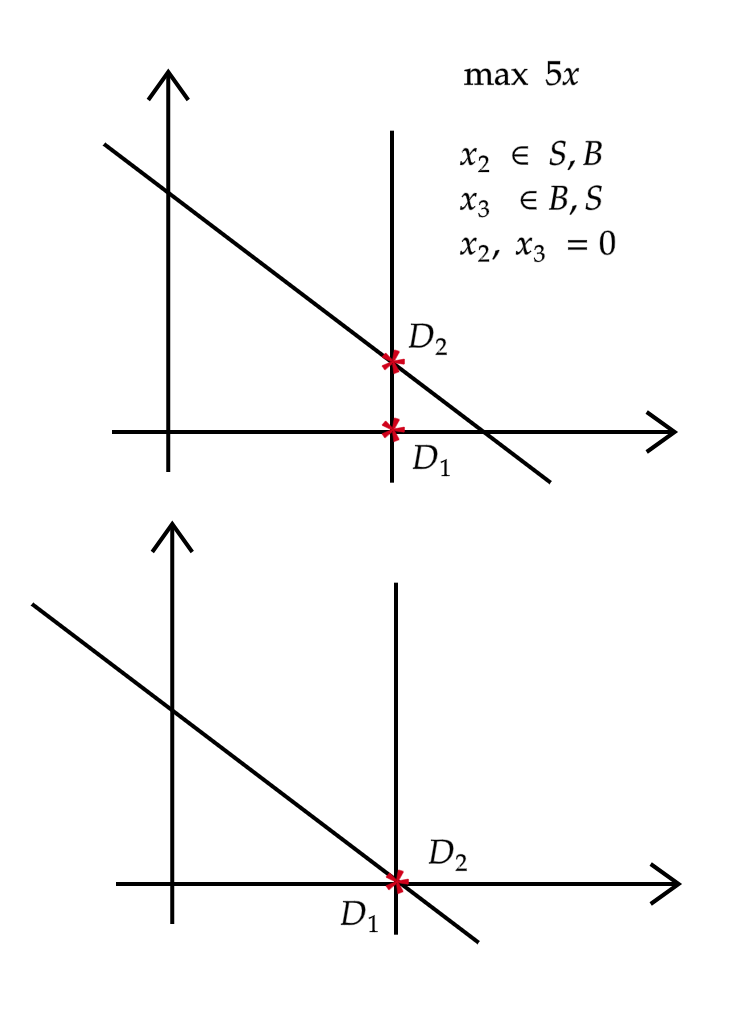
\includegraphics[width=\textwidth]{fig-17.png}
		\end{center}
	\end{marginfigure}

	\subsection{The Simplex Algorithm: Initialization}
	\begin{defn}[Auxiliary Problem]
		Given a linear program,
		\[
				\begin{array}{cc}
				\operatorname{maximize} & \sum_{j = 1}^n c_jx_j \\
				\text{ subject to } & \sum_{j=1}^{n} a_{i j} x_{j} \leq b_{i} \quad(i \in [m]) \\
				& x_{j} \geq 0 \quad(j \in [n]) 
			\end{array}
		\]
	\noindent the \textbf{auxiliary problem} is defined as,
		\[
			\begin{array}{cc}
				\operatorname{minimize} & x_{0} \\
				\text{ subject to } & \sum_{j=1}^{n} a_{i j} x_{j}-x_{0} \leq b_{i} \quad(i \in [m]) \\
				& x_{j} \geq 0 \quad(j \in [n]) 
			\end{array}
		\]
	\end{defn}

	\begin{ex}{Initialization}{label}
		The \textbf{all-zero} solution is not always feasible,
		\[
		\begin{array}{cccccccc}
		\operatorname{maximize} & x_{1} & - & x_{2} & + & x_{3} & \\
		\text { subject to } & 2 x_{1} & - & x_{2} & + & 2 x_{3} & \leq & 4 \\
		& 2 x_{1} & - & 3 x_{2} & + & x_{3} & \leq & -5 \\
		& -x_{1} & + & x_{2} & - & 2 x_{3} & \leq & -1 \\
		& & & x_{1}, & x_{2}, & x_{3} & \geq & 0
		\end{array}
		\]
	\end{ex}

	\begin{rmk}
		The original problem has a feasible solution if and only if the optimum value of the auxiliary problem is zero\footnote{We solve the auxiliary problem first.}.
	\end{rmk}


	\subsection{The Simplex Algorithm: Efficiency}
	\begin{marginfigure}
		\textbf{(Conjecture)}
		The simplex algorithm is polynomial time if, given a choice, it chooses the pivot variables at random.
	\end{marginfigure}

	\begin{thm}
		With Bland's Rule, the simplex algorithm terminates in,
		\[\binom{m+n}{m} >> 2^{m+n} \quad \text{iterations.}\]
	\end{thm}

	\begin{proof}
		This follows from the fact that there are $\binom{m+n}{m}$ bases cases, and the dictionary corresponding to each basis can only appear once.
	\end{proof}

	\begin{rmk}
		The simplex algorithm typically makes $O(m)$ pivots, where $m$ is the number of constraints\footnote{Since the number of constraints in the dual is the number of variables in the primal, $O(n)$ pivots are typically needed to solve the dual. If $n < m$, taking the dual gives a quicker solution.}.  Each pivot takes $O(mn)$ with dictionaries.
	\end{rmk}

	\subsection{Linear Programming Duality}
	\begin{thm}[Weak Duality Theorem]
		For any primal feasible solution $x$ and any dual feasible solution $y$, we have $c^Tx \leq b^Ty$.
	\end{thm}

	\begin{proof}
		Using the matrix encodings\footnote{$\geq$ applies to all entries.} of the linear programs $x$ and $y$,
		\begin{align*}
			c^T \cdot x &\leq (A^Ty)^T \cdot x \text{ since $A^{T}y \geq c$ and taking the transpose}\\
					 &= (y^TA) \cdot x \\
					 &= y^T \cdot (Ax) \\
					 &\leq y^T \cdot b \text{ by the dual feasibility of $x$}
		\end{align*}
	\end{proof}

	\begin{ex}{Duality}{label}
		Consider the primal,
		\[
			\begin{array}{cccccccccc}
			\operatorname{maximise} & 4x_{1} & + & x_{2} & + & 5x_{3} & + & 3x_{4} & & \\
			\text { subject to } & x_{1} & - & x_{2} & - & x_{3} & + & 3 x_{4} & \leq & 1
			\\ & 5 x_{1} & + & x_{2} & + & 3 x_{3} & + & 8 x_{4} & \leq & 55
			\\ & -x_{1} & + & 2 x_{2} & + & 3 x_{3} & - & 5 x_{4} & \leq & 3
			\\ & & & & x_{1}, & x_{2}, & x_{3} & , x_{4} & \geq & 0
			\end{array}
		\]
		\noindent and its dual,
		\[
		\begin{array}{ccccccccc}
		\operatorname{minimize} & y_{1} & + & 55 y_{2} & + & 3 y_{3} & &
		\\ \text { subject to } & y_{1} & + & 5 y_{2} & - & y_{3} & \geq & 4
		\\ & -y_{1} & + & y_{2} & + & 2 y_{3} & \geq & 1 \\
		& -y_{1} & + & 3 y_{2} & + & 3 y_{3} & \geq & 5
		\\ & 3 y_{1} & + & 8 y_{2} & - & 5 y_{3} & \geq & 3
		\\ & & & y_{1}, & y_{2} & y_{3} & \geq & 0
		\end{array}
		\]

		\noindent The primal has optimal solution,
		\[(x_1, x_2, x_3, x_4) = (0, 14, 0, 5) = 29\]
		\noindent The dual has optimal solution,
		\[(y_1, y_2, y_3) = (11,0,6) = 29\]
	\end{ex}

	\begin{thm}[Strong Duality Theorem]
		Let $x$ be an optimal primal solution and $y$ be an optimal dual solution\footnote{An optimal solution might not exist: \begin{itemize}
			\item The feasible region is empty
			\begin{itemize}
				\item $x_1 \leq 1$
				\item $x_2 \geq 2$
			\end{itemize}
			\item The optimal value is infinite
			\begin{itemize}
				\item $\max x_1 + x_2$
				\item $x_1, x_2 \geq 0$
			\end{itemize}
		\end{itemize}}. Then $c^Tx = b^Ty$.
	\end{thm}

	\begin{proof}
		The simplex algorithm finds the optimal primal solution. It has decision variables $(x_1^*, \cdots, x_n^*)$ and slack variables $(x_{n+1}^* \cdots, x_{n+m}^*)$. The top row of the final dictionary is,
		\[z = \texttt{OPT} - \sum_{k=1}^{n+m} \gamma_k x_k\]
		\noindent where $\gamma_k \geq 0$, with equality for basis variables. Define dual variables $y_i^* = \gamma_{n+i}$ for $i \in [m]$. We need to show that,
		\begin{enumerate}
			\item $(y_1^*, \cdots, y_m^*)$ is a feasible solution for the dual,
		\[\sum_{i=1}^m a_{ij}y_i^* \geq c_j \quad \forall j \in [n]\]
			\item The value of $(y_1^*, \cdots, y_m^*)$ is equal to the optimal primal value,
			\[\sum_{j=1}^{n} c_{j} \cdot x_{j}^{*}=\sum_{i=1}^{m} b_{i} \cdot y_{i}^{*}\]
		\end{enumerate}
		\noindent  Let $z^* = \texttt{OPT(primal)} = \sum_{j=1}^n c_j \cdot x_j^*$. The final dictionary states that,
		\begin{align*}
			z &= \sum_{j=1}^n c_j \cdot x_j^* - \sum_{k=1}^{n+m} \gamma_k \cdot x_k \\
			  &= z^* - \sum_{k=1}^{n+m} \gamma_k \cdot x_k \\
			  &= \texttt{OPT(primal)} - \sum_{k=1}^{n+m} \gamma_k \cdot x_k \\
			  &= \texttt{OPT(primal)} - \sum_{k=1}^{n} \gamma_k \cdot x_k \ - \sum_{k=n+1}^{n+m} \gamma_k \cdot x_k \\
			  &\text{Re-indexing the sum to work with the dual variables,} \\
			  &= \texttt{OPT(primal)} - \sum_{j=1}^{n} \gamma_j \cdot x_j \ - \sum_{i=1}^{m} \gamma_{n+i} \cdot x_{n+1} \\
			  &\text{Since $y_i^* = \gamma_{n+i}$ for $i \in [m]$ by definition of the optimal dual solution,} \\
			  &= \texttt{OPT(primal)} - \sum_{j=1}^{n} \gamma_j \cdot x_j \ - \sum_{i=1}^{m} y_i^* \cdot x_{n+1} \\
			  &\text{But $x_{n+i}$ are our slack variables,} \\
			  &= \texttt{OPT(primal)} - \sum_{j=1}^{n} \gamma_j \cdot x_j \ - \sum_{i=1}^{m} y_i^* \cdot \bigg(b_i - \sum_{j=1}^n a_{ij} \cdot x_j\bigg) \\
			  &\text{Re-arranging,} \\
			  &= \bigg(\texttt{OPT(primal)} - \sum_{i=1}^m b_i \cdot y_i^*\bigg) + \sum_{j=1}^n \bigg(\sum_{i=1}^m a_{ij}y_i^* - \gamma_j\bigg) \cdot x_j
		\end{align*}
		\noindent Since this equality holds for all choices of $\{x_1, \cdots x_n\}$,
		\[c_j = \sum_{i=1}^m a_{ij} \cdot y_i^* - \gamma_j\]
		\noindent But $\gamma_j \geq 0$, so we have feasibility,
		\[\sum_{i=1}^m a_{ij} \cdot y_i^* \geq c_j\]
		\noindent and it must be that,
		\[\texttt{OPT(primal)} - \sum_{i=1}^m b_i \cdot y_i^* = 0\]
		\noindent so we have strong duality,
		\[\sum_{i=1}^{m} b_{i} \cdot y_{i}^{*}=0 = \texttt{OPT(primal)}=\sum_{j=1}^{n} c_{j} \cdot x_{j}^{*}\]
	\end{proof}
	
	\begin{rmk}
		The primal is infeasible if the optimal of the dual is $-\infty$ or $\infty$.
	\end{rmk}

	\begin{thm}[Completemenary Slackness Theorem]
		TFAE,
		\begin{itemize}
			\item $x$ and $y$ are optimal solutions
			\item $c \cdot x = y \cdot b$
			\item $c \cdot x = yAx$
			\item $yAx = y \cdot b$
			\item $x$ and $y$ satisfy the complementary slackness conditions
		\end{itemize}
	\end{thm}

	\begin{proof}
		This is a result of strong duality.
	\end{proof}

	\subsection{Applications of Linear Programming}

	\begin{marginfigure}
		Linear programs can model \textbf{Boolean combinatorial circuits}. For each gate $g$, there is a variable $0 \leq x_g \leq 1$. Then,
		\begin{itemize}
			\item \texttt{INPUT} gates are set to their input

			\begin{center}
				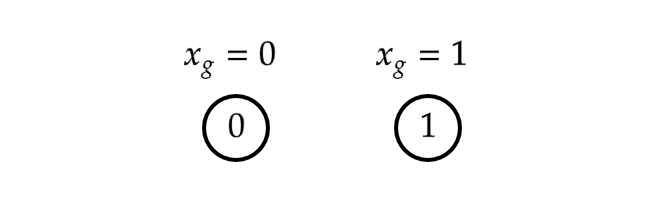
\includegraphics[width=\textwidth]{fig-5.png}
			\end{center}
			
			\item \texttt{NOT} gates are set to the opposite

			\begin{center}
				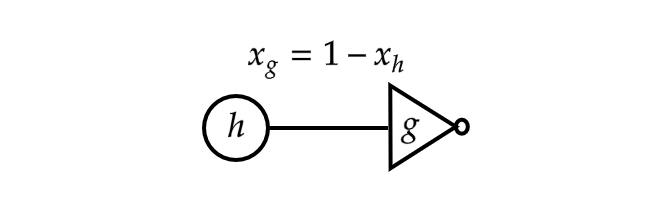
\includegraphics[width=\textwidth]{fig-6.png}
			\end{center}
			
			\item \texttt{OR} gates are set $\max \{x_{h_1}, x_{h_2}\}$

			\begin{center}
				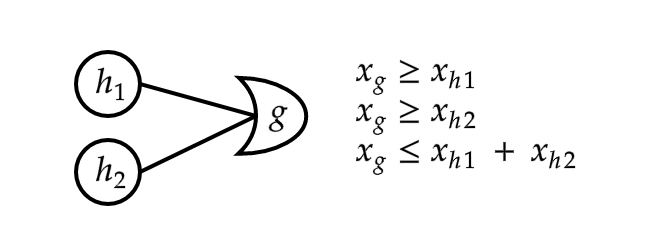
\includegraphics[width=\textwidth]{fig-7.png}
			\end{center}
			
			\item \texttt{AND} gates are set to $\min \{x_{h_1}, x_{h_2}\}$

			\begin{center}
				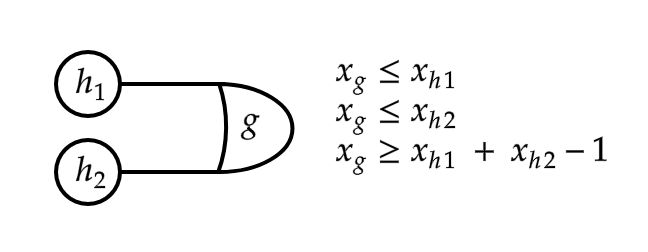
\includegraphics[width=\textwidth]{fig-8.png}
			\end{center}
			
			
		\end{itemize}
	\end{marginfigure}

	\begin{ex}{Matching as a Motivating Example}{label}
		Let $G = (V, E)$ be an undirected graph. The integer formulation of the \textbf{matching problem} is,
		\begin{itemize}
			\item An edge $e$ in the graph is picked if $x_e = 1$,
			\[x_e \in \{0,1\} \quad \forall e \in E\]
			\item We want to maximize the number of edges in the matching,
			\[\max \sum_{e \in E} x_e\]
			\item One edge is incident to each vertex,
			\[\sum_{e \in \delta(v)} x_e \leq 1 \quad \forall e \in E\]
		\end{itemize}
		\noindent In summary,
		\[
			\begin{array}{lll}
				\operatorname{maximize} & \sum_{e \in E} x_{e} & \\
				\text{ subject to } & \sum_{e \in \delta(v)} x_{e} \leq 1 & \quad \forall v \in V \\
				& x_{e} \in\{0,1\} & \quad \forall e \in E
			\end{array}
		\]
		\noindent We do not have a polynomial time algorithm for solving integer programs. If we relax the integrality constraints,
		\[
			\begin{array}{lll}
				\operatorname{maximize} & \sum_{e \in E} x_{e} & \\
				\text{ subject to } & \sum_{e \in \delta(v)} x_{e} \leq 1 & \quad \forall v \in V \\
				& x_{e} \geq 0 & \quad \forall e \in E
			\end{array}
		\]
		\noindent we may obtain a fractional solution,
		\begin{center}
			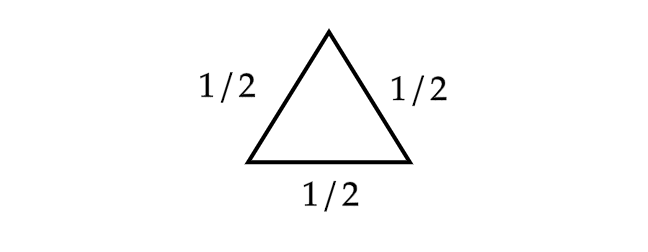
\includegraphics[width=0.45\textwidth]{fig-9.png}
		\end{center}
	\end{ex}

	\begin{marginfigure}
		Recall the following,
		\begin{itemize}
			\item The simplex algorithm outputs a basic solution, which is an extreme point of the feasible region.
			\item The feasible region is the convex hull of the extreme points.
			\item A basic solution is not a convex combination of two feasible ones.
		\end{itemize}
		\noindent where a \textbf{convex combination} is a linear combination of points where all coefficients are non-negative and sum to 1.
	\end{marginfigure}

	\begin{thm}[Bipartite Matching]
		Bipartite graphs have an optimal integral solution to the following linear program,
		\[
			\begin{array}{lll}
				\operatorname{maximize} & \sum_{e \in E} x_{e} & \\
				\text{ subject to } & \sum_{e \in \delta(v)} x_{e} \leq 1 & \quad \forall v \in V \\
				& x_{e} \geq 0 & \quad \forall e \in E
			\end{array}
		\]
	\end{thm}

	\begin{proof}
		Let $x$ be a basic solution to our linear program. We need to show that $x_e \in \{0,1\}$ for all $e \in E$. Suppose not. Then, $x_e \in (0,1)$ for all $e \in E$. If $x_e = 0$, then we can recurse on $G - \{e\}$ to produce a strictly fractional collection of $x_e$ values. Similarly, if $x_e = 1$, then we can recurse on $G - e$ since no edge adjacent to $e$ will produce a matching on this subgraph.
		\begin{itemize}
			\item \textbf{Case 1.} $G$ contains a cycle $C$.
			\begin{itemize}
				\item $C$ contains an even number of edges, and therefore we can partition $C$ into two equal sized matchings $M_1, M_2$
				\item Define two linear programs $y, z$ as follows,
				\[
				y_{e}=\left\{\begin{array}{ll}x_{e}+\epsilon & \text { if } e \in M_{1} \\ x_{e}-\epsilon & \text { if } e \in M_{2} \\ x_{e} & \text { if } e \notin C\end{array} \quad \quad z_{e}= \begin{cases}x_{e}-\epsilon & \text { if } e \in M_{1} \\ x_{e}+\epsilon & \text { if } e \in M_{2} \\ x_{e} & \text { if } e \notin C\end{cases}\right.
				\]
				\item Observe that $x$ is a convex combination of $y$ and $z$,
				\[x = \frac{1}{2} \cdot (y + z)\]
				\item Furthermore, $x$ is fractional,
				\[0 < x_e < 1 \quad \forall e \in E\]
				\item Thus, we can pick $\epsilon$ such that both $y$ and $z$ are fractional,
				\[0<y_{e}<1 \quad \forall e \in E \quad \quad \quad 0<z_{e}<1 \quad \forall e \in E\]
				\item Adding and subtracting $\epsilon$ along the red, we see that,
				\[\forall v \in V \quad \sum_{e \in \delta(v)} x_{e}=\sum_{e \in \delta(v)} y_{e}=\sum_{e \in \delta(v)} z_{e} \leq 1\]
				\item This implies that $x$ is a convex combination of two feasible solutions. Thus, $x$ is not a basic solution.
			\end{itemize}

			\item \textbf{Case 2.} $G$ is acyclic, i.e., $G$ is a forest.
			\begin{itemize}
				\item Let $P$ be a maximal path in $G$. We can partition $P$ into two matchings $P_1, P_2$ and define two linear programs $y, z$,
				\[y_{e}=\left\{\begin{array}{ll}x_{e}+\epsilon & \text { if } e \in P_{1} \\ x_{e}-\epsilon & \text { if } e \in P_{2} \\ x_{e} & \text { if } e \notin P\end{array} \quad \quad z_{e}= \begin{cases}x_{e}-\epsilon & \text { if } e \in P_{1} \\ x_{e}+\epsilon & \text { if } e \in P_{2} \\ x_{e} & \text { if } e \notin P\end{cases}\right.\]
				\item Repeating the same argument from Case 1 with $x = \frac{1}{2} \cdot (y + z)$,
				\[0<y_{e}<1 \quad \forall e \in E \quad \quad \quad 0<z_{e}<1 \quad \forall e \in E\]
				\item For any vertex $v \in V \{v_{1}, v_{2}\}$,
				\[\forall v \in V \backslash\left\{v_{1}, v_{2}\right\} \quad \sum_{e \in \delta(v)} x_{e}=\sum_{e \in \delta(v)} y_{e}=\sum_{e \in \delta(v)} z_{e} \leq 1\]
				\item $v_1$ is necessarily a leaf, meaning that it is incident to one edge,
				\[\sum_{e \in \delta\left(v_{1}\right)} y_{e}<1 \quad \sum_{e \in \delta\left(v_{1}\right)} z_{e}<1\]
				\item Since the same holds for $v_2$, $x$ is a convex combination of two feasible solutions. Thus, $x$ is not a basic solution.
			\end{itemize}
		\end{itemize}
		\noindent Hence, the optimal solution to the program is integral.
	\end{proof}

	\begin{cor}
		A similar argument shows that we can solve the \textbf{maximum weight matching problem} for bipartite graphs in polynomial time,
		\[
			\begin{array}{lll}
				\operatorname{maximize} & \sum_{e \in E} w_e \cdot x_{e} & \\
				\text{ subject to } & \sum_{e \in \delta(v)} x_{e} \leq 1 & \quad \forall v \in V \\
				& x_{e} \geq 0 & \quad \forall e \in E
			\end{array}
		\]
	\end{cor}

	\begin{marginfigure}
		$A$ is the incidence matrix, 
		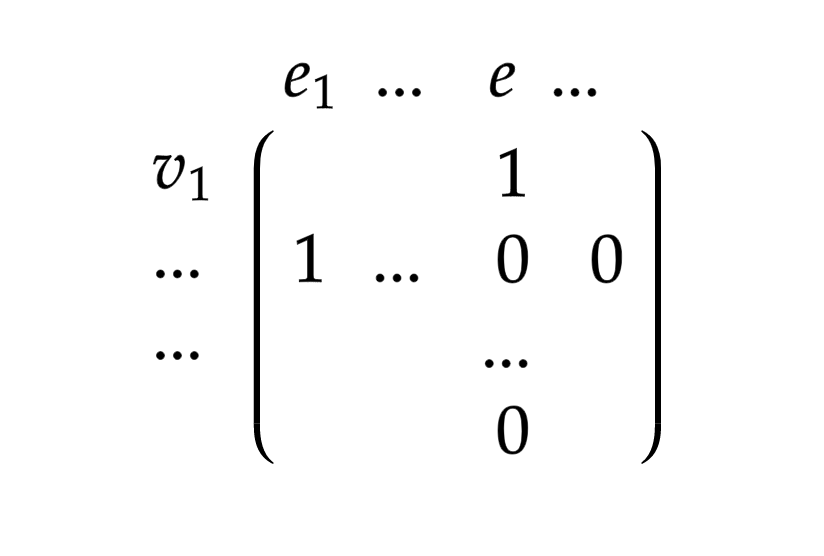
\includegraphics[width=0.8\textwidth]{fig-10.png}
	\end{marginfigure}

	\begin{rmk}
		The matrix encoding of the dual linear program is,
		\[
		   \min \underbrace{\Set{ 1^Ty \ | \begin{array}{l}
		    A^T y \geq c \\
		    y \geq 0
		  \end{array}}}_{Dual}
			\iff
			\max \underbrace{\Set{ 1^Tx \ | \begin{array}{l}
		    Ax \leq 1 \\
		    x \geq 0
		  \end{array}}}_{Primal}
		\]
		\noindent allowing us to re-interpret the dual as the \textbf{vertex cover problem},
		\[
		\begin{array}{lll}
				\operatorname{minimize} & \sum_{v \in V} y_v & \\
				\text{ subject to } & y_u + y_v \geq 1 & \quad \forall (u,v) \in E \\
				& y_v \geq 0 & \quad \forall v \in V
			\end{array}
		\]
	\end{rmk}

	\begin{ex}{The Shortest Path Problem}{label}
		Given a directed graph $G = (V, A)$ with a source vertex $s$ and a sink vertex $t$, we can set up the shortest path problem,
		\begin{itemize}
			\item Let each arc $a \in A$ have non-negative length $l_a$
			\item The length of a path $P$ is,
			\[l(P) = \sum_{a \in P}l_a\]
		\end{itemize}
		We can formulate this as an \textbf{integer program},
		\[
		\begin{array}{ll}
				\operatorname{minimize} & \sum_{a \in A} \ell_{a} \cdot x_{a} \\
				\text{ subject to } & x_{a} \in\{0,1\} \quad \forall a \in A \\
				& \sum_{a \in \delta^{-}(v)} x_{a}-\sum_{a \in \delta+(v)} x_{a}= \begin{cases}-1 & v=s \\
												0 & v \neq\{s, t\} \\
												1 & v=t\end{cases}
			\end{array}
		\]
		\noindent and do a constraint relaxation.
	\end{ex}

	\begin{thm}[Shortest Path]
		The shortest path problem has an optimal integral solution to the following linear program,
		\[
		\begin{array}{ll}
				\operatorname{minimize} & \sum_{a \in A} \ell_{a} \cdot x_{a} \\
				\text{ subject to } & x_{a} \geq 0 \quad \forall a \in A \\
				& \sum_{a \in \delta^{-}(v)} x_{a}-\sum_{a \in \delta+(v)} x_{a}= \begin{cases}-1 & v=s \\
												0 & v \neq\{s, t\} \\
												1 & v=t\end{cases}
			\end{array}
		\]
	\end{thm}

	\begin{proof}
		Any basic solution $x$ represents an $(s-t)$ flow of value $1$. By the Flow Decomposition Theorem, $x$ decomposes into $(s,t)$ paths,
		\begin{align*}
			&\mathbf{x}=\alpha_{1} \cdot P_{1}+\alpha_{2} \cdot P_{2}+\cdots+\alpha_{k} \cdot P_{k} \\
			&\text{where } \sum_{i=1}^{k} \alpha_{i}=1 \text{ and } \alpha_{i} \geq 0 \quad \forall i
		\end{align*}
		\noindent 
	\end{proof}
	\noindent but each $P_i$ is a feasible solution to the linear program. Either we have a contradiction, or $k = 1$. If $k = 1$, then $x$ is an $(s-t)$ path itself and is an integral solution.

	\begin{marginfigure}
		$A_{ij}$ is negative if $v_i$ is the tail of $a_j$,
		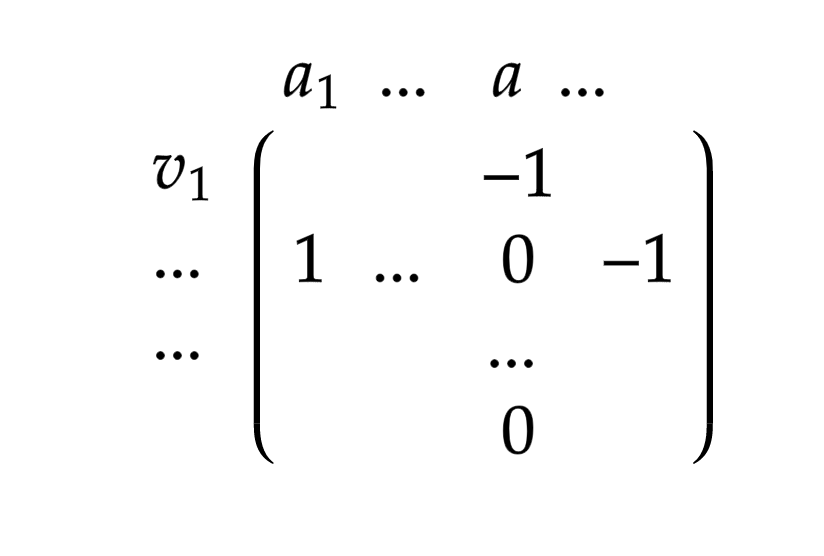
\includegraphics[width=0.8\textwidth]{fig-11.png}
	\end{marginfigure}

	\begin{rmk}
		The matrix encoding of the dual linear program, even though the primal is not in standard form, is,
		\[\max \Set{ y_t - y_s \ | \begin{array}{l}
		    y_v \text{ unrestricted } \quad \forall v \in V  \\
		    A^Ty \leq l
		  \end{array}}\]
		\noindent Changing labels of $y$ to $d$ to represent distances,
		\[\max \Set{ d_t - d_s \ | \begin{array}{l}
		    d_v \text{ unrestricted } \quad \forall v \in V  \\
		    d_v - d_u \leq l_{uv} \quad \forall a = (u,v) \in A
		  \end{array}}\]
		\noindent setting $d_s = 0$, we see that $d_v$ is the distance from $v$ to $s$.
	\end{rmk}

	\begin{ex}{Maximum Flow Problem}{label}
		Recalling our formulation of maximum flow,
		\[
		\begin{array}{ll}
				\operatorname{maximize} & \sum_{a \in \delta^-(t)} f_{a} \\
				\text{ subject to } & 0 \leq f_a \leq u_a \quad \forall a \in A \\
				& \sum_{a \in \delta^{-}(v)} f_{a} = \sum_{a \in \delta^{+}(v)} f_{a} \quad \forall v \in V - \{s,t\}
			\end{array}
		\]
	\end{ex}

	\begin{ex}{Zero-Sum Games}{label}
		The \textbf{Minimax Theorem} is a result of the linear programming duality. It states that for any matrix $A$,
		\[\max _{\mathbf{x}}\left[\min _{\mathbf{y}} \mathbf{x}^{T} A \mathbf{y}\right]=\min _{\mathbf{y}}\left[\max _{\mathbf{x}} \mathbf{x}^{T} A \mathbf{y}\right]\]
	\end{ex}

\section{Computational Complexity}
  
	\subsection{Polynomial-Time Reductions}
	A reduction $Q \leadsto R$ from a problem $Q$ to another problem $R$ represents $Q$ as a case of $R$, which we already know how to solve. Examples of reductions that we have seen are,
	\begin{align*}
		&\text{Bipartite Matching $\leadsto$ Maximum Flow} \\
		&\text{Bipartite Vertex Cover $\leadsto$ Minimum Cut} \\
		&\text{Maximum Flow $\leadsto$ Linear Programming}
	\end{align*}

	\begin{defn}[Karp Reductions]
		A \textbf{Karp reduction} $Q \leadsto R$ from $Q$ to $R$ is an algorithm that produces an instance \texttt{I'} of $R$ given an instance $\texttt{I}$ of $R$. The algorithm runs in polynomial time in the size of \texttt{I} and \texttt{I'} is a \texttt{YES} instance of $R$ if and only if $\texttt{I}$ is a \texttt{YES} instance of $Q$\footnote{We write $Q \leq_p R$, which can be read as "$Q$ is polynomial-time reducible to $R$" or "$R$ is at least as hard as $Q$."}.
	\end{defn}

	\begin{rmk}
		Let $Q \leadsto R$. 
		\begin{itemize}
			\item If $R$ is easy to solve, then $Q$ is easy to solve
			\[R_{\texttt{easy}} \implies Q_{\texttt{easy}}\]
			\item If $Q$ is hard to solve, then $R$ is hard to solve
			\[Q_{\texttt{hard}} \implies R_{\texttt{hard}}\]
			\item If $Q$ is easy to solve, then this tells us nothing about $R$ 
			\[Q_{\texttt{hard}} \implies \text{Nothing}\]
		\end{itemize}
	\end{rmk}

	\begin{defn}[Vertex Cover Problem]
		We are given a graph $G = (V, E)$ and an integer $c$. We want to know if $G$ contains a set of at most $c$ vertices that are incident to each edge.
	\end{defn}

	\begin{defn}[Independent Set Problem]
		We are given a graph $G = (V, E)$ and an integer $k$. We want to know if $G$ contains a set of at least $k$ vertices that are mutually non-adjacent.
	\end{defn}

	\begin{ex}{Independent Set $\leadsto$ Vertex Cover}{label}
		If $S \subseteq V$ is an independent set, then $V - S$ is a vertex cover. A polynomial time algorithm for \textbf{Vertex Cover} can be used to give a polynomial time algorithm for \textbf{Independent Set}.
		\begin{align*}
			\text{There is an independent set of size at least $k$}
		\end{align*}
		\[\iff\]
		\begin{align*}
			\text{There is a vertex cover of size at most $n-k$}
		\end{align*}
		\noindent Similarly, Vertex Cover $\leadsto$ Independent Set.
	\end{ex}

	\begin{defn}[Set Cover Problem]
		We are given sets $S_1, S_2, \cdots, S_n \subseteq W$ and an integer $k$. We want to know if there is a collection of at most $k$ sets that cover every element of $W$.
	\end{defn}

	\begin{ex}{Vertex Cover $\leadsto$ Set Cover}{label}
		Suppose that we are given a graph $G = (V, E)$. Define,
		\[S_v := \{e \text{ $|$ $v$ is an endpoint of $e$}\}\]
		\noindent for each $v \in V$. Set $W = \{e \text{ $|$ } e \in E\}$. Then a set cover of size $k$ corresponds to a vertex cover of size $k$, and a polynomial time algorithm for \textbf{Set Cover} can be used to give a polynomial time algorithm for \textbf{Vertex Cover}.
	\end{ex}

	\begin{defn}[Satisfiability Problem]
		Suppose that we have,
		\begin{itemize}
			\item Boolean variables $x_1, \cdots, x_n$
			\item Clauses $C_1, \cdots, C_m$ which are disjunctions of literals,
			\[C_{j}=x_{2} \lor \bar{x}_{5} \lor \bar{x}_{6} \lor x_{8} \lor \bar{x}_{9}\]
			\item Literals $x_i$ and $\bar{x_i} \in \{\texttt{True}, \texttt{False}\}$ for each variable $x_i$
		\end{itemize}
		\noindent We want to know if there is an assignment that satisfies every clause.
	\end{defn}

	\begin{defn}[3-Satisfiability]
		\textbf{3-satisfiability} is a special case of the satisfiability problem, where every clause has exactly three literals.
		\[\text{e.g., }\quad \left(x_{1} \lor \bar{x}_{2} \lor x_{5}\right) \wedge\left(x_{2} \lor \bar{x}_{3} \lor \bar{x}_{4}\right) \wedge\left(\bar{x}_{1} \lor x_{3} \lor x_{4}\right) \wedge\left(\bar{x}_{3} \lor \bar{x}_{4} \lor \bar{x}_{5}\right)\]
	\end{defn}

	\begin{ex}{SAT $\leadsto$ 3-SAT}{label}
		Clearly SAT $\leadsto$ 3-SAT. We can also show that SAT $\leadsto$ 3-SAT. 
		
		\begin{rmk}
		A variable assignment satisfies $\ell_1 \lor \ell_2 \lor \cdots \lor \ell_k$ if and only if the same variable assignment satisfies,
		\[\left(\ell_{1} \lor \cdots \lor \ell_{p} \lor y\right) \wedge\left(\bar{y} \lor \ell_{p+1} \lor \cdots \lor \ell_{k}\right)\]
		\noindent for some \texttt{True} / \texttt{False} assignment of $y$.
		\label{satisfiability}
	\end{rmk}

		\begin{itemize}
			\item We need to convert an instance \texttt{I} of SAT into an instance \texttt{I'} of 3-SAT. To do this, take each clause $C$ in \texttt{I} and mimic it via a set of clauses of size 3 with additional variables
			\item Take a clause $C = \ell_{1} \lor \ell_{2} \lor \cdots \ell_{k}$. There are three cases,
			\begin{itemize}
				\item If $k = 2$, we can pick $y$ and $\bar{y}$ as follows:
				
				\resizebox{.6\hsize}{!}{
				$\ell_{1} \lor \ell_{2} \quad \Longrightarrow \quad\left(\ell_{1} \lor \ell_{2} \lor y\right) \wedge\left(\ell_{1} \lor \ell_{2} \lor \bar{y}\right)$}

				\item If $k = 1$, we can pick $y_1, y_2$ and $\bar{y_1}, \bar{y_2}$ as follows:
				
				\resizebox{.9\hsize}{!}{
				$\ell_{1} \implies \left(\ell_{1} \lor y_{1} \lor y_{2}\right) \wedge\left(\ell_{1} \lor y_{1} \lor \bar{y}_{2}\right) \wedge\left(\ell_{1} \lor \bar{y}_{1} \lor y_{2}\right) \wedge\left(\ell_{1} \lor \bar{y}_{1} \lor \bar{y}_{2}\right)$}

				\item If $k \geq 3$, we apply Remark \ref{satisfiability} recursively.
			\end{itemize}
		\end{itemize}.
		Thus, for $C = \ell_{1} \lor \ell_{2} \lor \cdots \ell_{k}$, we have:
		\begin{itemize}
			\item $k - 2$ clauses in \texttt{I'}
			\item $k - 3$ new variables in \texttt{I'}
		\end{itemize}
		so a polynomial time algorithm for \textbf{3-SAT} can be used to give a polynomial time algorithm for \textbf{SAT}.
	\end{ex}

	\begin{ex}{3-SAT $\leadsto$ Independent Set}{label}
		\begin{itemize}
			\item We need to convert an instance \texttt{I} of 3-SAT,
			\[C=x_{1} \vee \bar{x}_{2} \vee x_{5}\]
			\noindent into an instance \texttt{G} of Independent Set. For each clause $C$ in \texttt{I}, we have a triangle in \texttt{G},

			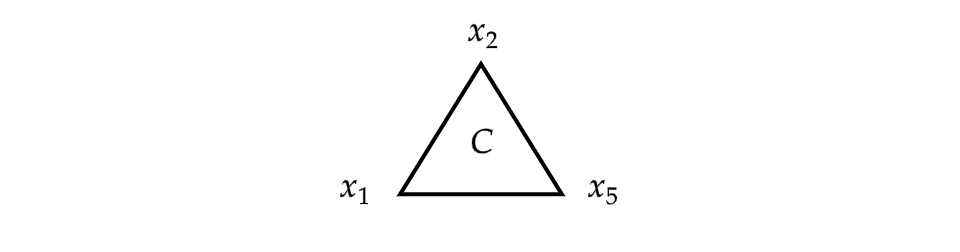
\includegraphics[width=\textwidth]{fig-12.png}

			\item We add an edge between each copy of $x_i$ and $\bar{x_i}$,

			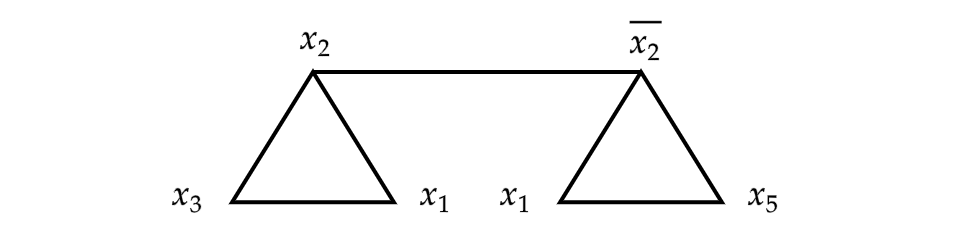
\includegraphics[width=\textwidth]{fig-13.png}
		\end{itemize}
		There is a satisfying assignment for \texttt{I} if and only if there is an independent set in $G$ whose size is equal to the number of clauses. To see this, note that,
		\begin{itemize}
			\item There are $m$ triangles in $G$ and an independent set $S$ uses at most one vertex per triangle. This means that,
			\[|S| \leq m\]
			\item If $S$ selects $x_i$, then $x_i$ is set to \texttt{True}. We cannot also select a vertex for $x_i$, so $S$ induces a valid assignment
			\item If $S$ selects $x_i \in C_j$, then $C_j$ is satisfied
			\item Thus, an independent set of size $m$ in $G$ gives a satisfying assignment for \texttt{I} and any satisfying assignment for \texttt{I} induces an independent set of size $m$ in $G$ 
		\end{itemize}
 	\end{ex}

 	\subsection{NP Completeness}
 	\begin{marginfigure}
 		Equivalently, $NP$ is,
 		\begin{itemize}
 			\item The set of decision problems whose \texttt{YES} instances can be verified in polynomial time
 			\item The set of decision problems that can be solved in exponential time by Brute-Force Search
 		\end{itemize}
 		\noindent These definitions are equivalent because any \texttt{YES} instance has a certificate of size $poly(n)$, and there are an exponential, i.e., $2^{poly(n)}$ number of such certificates.
 	\end{marginfigure}

 	\begin{defn}[P]
 		The class \textbf{P} is the set of decision problems which can be solved in polynomial time by a deterministic computer.
 	\end{defn}

 	\begin{defn}[NP]
 		The class \textbf{NP} is the set of decision problems which can always be solved in polynomial time by a non-deterministic computer.
 	\end{defn}

 	\begin{rmk}[$P \neq NP$]
 		The \textbf{conjecture} that $P \neq NP$ states that computation is harder than verification. We know that $P \subseteq NP$ since we can compute and verify a solution to a problem $R \in P$ in polynomial time.
 	\end{rmk}

 	\begin{defn}[NP Complete]
 		A problem $R$ is \textbf{NP Complete} if for every $Q \in NP$, there is a polynomial time reduction\footnote{The reduction maps \texttt{YES} instances of $Q$ into \texttt{YES} instances of $R$, and it maps \texttt{NO} instances of $Q$ into \texttt{NO} instances of $R$} from $Q$ to $R$.
 	\end{defn}

 	 \begin{defn}[coNP]
 	 	 The class \textbf{coNP} is the set of decision problems whose \texttt{NO} instances can be verified in polynomial time.
 	\end{defn}

 	\begin{defn}[coNP Complete]
 		A problem $R$ is \textbf{coNP Complete} if for every $Q \in coNP$, there is a polynomial time reduction from $Q$ to $R$.
 	\end{defn}

 	\begin{defn}[Good Characterization]
 		A problem $R \in NP \cap coNP$ has a \textbf{good characterization} if has a polynomial \texttt{YES} and \texttt{NO} certificate.  
 	\end{defn}

 	\begin{ex}{Good Characterizations}{label}
 		The following problems have a good characterization,

 		\vphantom{.}

 		\resizebox{\textwidth}{!}{
 		\begin{tabular}{lll}
 		\textbf{Problem} & \textbf{\texttt{YES} Instance} & \textbf{\texttt{NO} Instance} \\ \hline
 		Maximum Flow & Flow & Minimum Cut \\
 		Bipartite Matching & Matching & Vertex Cover \\
 		Linear Programming & Feasible Primal & Feasible Dual \\
		\end{tabular}}
 	\end{ex}

 	\begin{rmk}
 		The complement of an NP Complete problem is in coNP.
 	\end{rmk}

 	\begin{rmk}
 		$P = NP \implies NP = coNP$
 	\end{rmk}

 	\begin{proof}
 		Problems in $P$ have a \texttt{YES} and \texttt{NO} certificate. If $P = NP$ then every problem in $NP$ has a short \texttt{YES} and \texttt{NO}. This implies,
 		\[P \subseteq coNP\]
 		\noindent Any problem $R \in coNP$ has $R^c \in NP = P \implies R \in P = NP$.
 	\end{proof}

 	\begin{ex}{Cliques}{label}
 		The problem of determining if a set $S$ of vertices is a clique is in NP. We can check if the vertices are pairwise adjacent, which is polynomial in the size of $S$.
 	\end{ex}

 	\begin{marginfigure}
 		\begin{center}
 						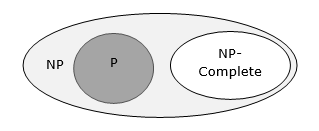
\includegraphics[width=\textwidth]{fig-16.png}
 			\end{center}
 	\end{marginfigure}

 	\begin{defn}[Cook's Theorem]
 		Satisfiability is NP Complete.
 	\end{defn}

 	\begin{marginfigure}
 		$3-SAT$, Independent Set, Vertex Cover, and Set Cover are NP Complete.
 	\end{marginfigure}

 	\begin{rmk}[Proving NP Completeness]
 		Do the following,
 		\begin{enumerate}
 			\item For your new problem $R$, show that $R \in NP$
 			\item Find an $NP$-complete problem $Q$ such that $Q \leadsto R$
 		\end{enumerate}
 	\end{rmk}

 	\begin{defn}[Graph-Coloring Problem]
 		A \textbf{vertex coloring} of a graph $G = (V,E)$ is an assignment of colors to vertices such that adjacent vertices recieve different colors. The chromatic number $\chi(G)$ is the minimum number of colors required for a valid coloring to exist. We want to know if there exists a 3-coloring of $G$.
 	\end{defn}

 	\begin{ex}{3-SAT $\leadsto$ 3-Coloring}{label}
 		First, we can show that 3-coloring is in NP by checking,
 		\begin{itemize}
 			\item $\leq 3$ colors are used
 			\item Every vertex recieves a color $c$
 			\item $c(u) \neq c(v)$ for all $(u,v) \in E$
 		\end{itemize}
 		
 		Second, we reduce from $3-SAT$ to 3-Coloring:
 		\begin{itemize}
 			\item We need to convert an instance \texttt{I} of 3-SAT into an instance \texttt{I'} of 3-Coloring. To do this, we build a graph $G$ as follows,
 			\begin{itemize}
 				\item There is a vertex for each literal $x_1, \bar{x_1}, x_2, \cdots, x_n, \bar{x_n}$
 				\item There are three vertices, $T, F, B$
 				\item The vertices are connected as follows,
 					\begin{center}
 						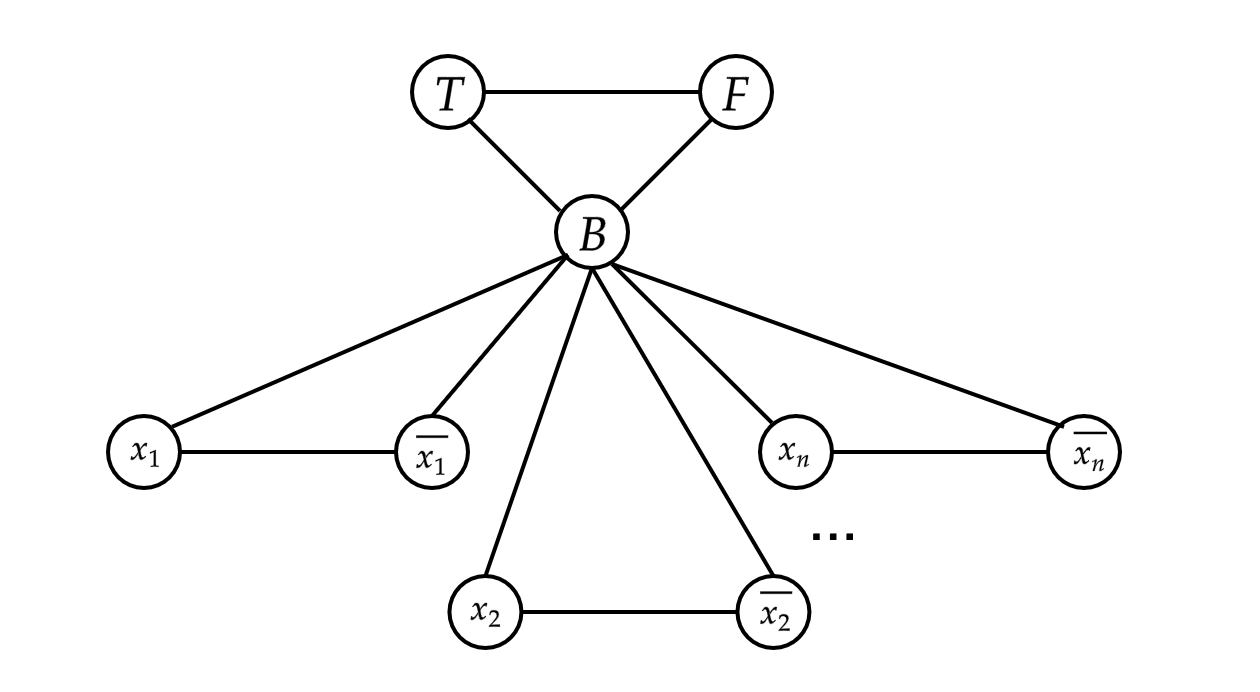
\includegraphics[width=0.5\textwidth]{fig-14.png}
 					\end{center}
 			\end{itemize}
 			\item Define the following,
 				\begin{itemize}
 					\item $\texttt{Green} = \texttt{True}$
 					\item $\texttt{Red} = \texttt{False}$
 					\item $\texttt{White} = \texttt{BLANK}$
 				\end{itemize}
 			\noindent so that the colors of $x_1, \bar{x_1}, x_2, \cdots, x_n, \bar{x_n}$ give a valid \texttt{True} and \texttt{False} assignment of variables.
 			
 			\item Design a gadget for each clause which can be 3-colored if and only if the clause is satisfied. Each gadget clause contains 6 new vertices which we connect to the assignment
 			 \begin{center}
 						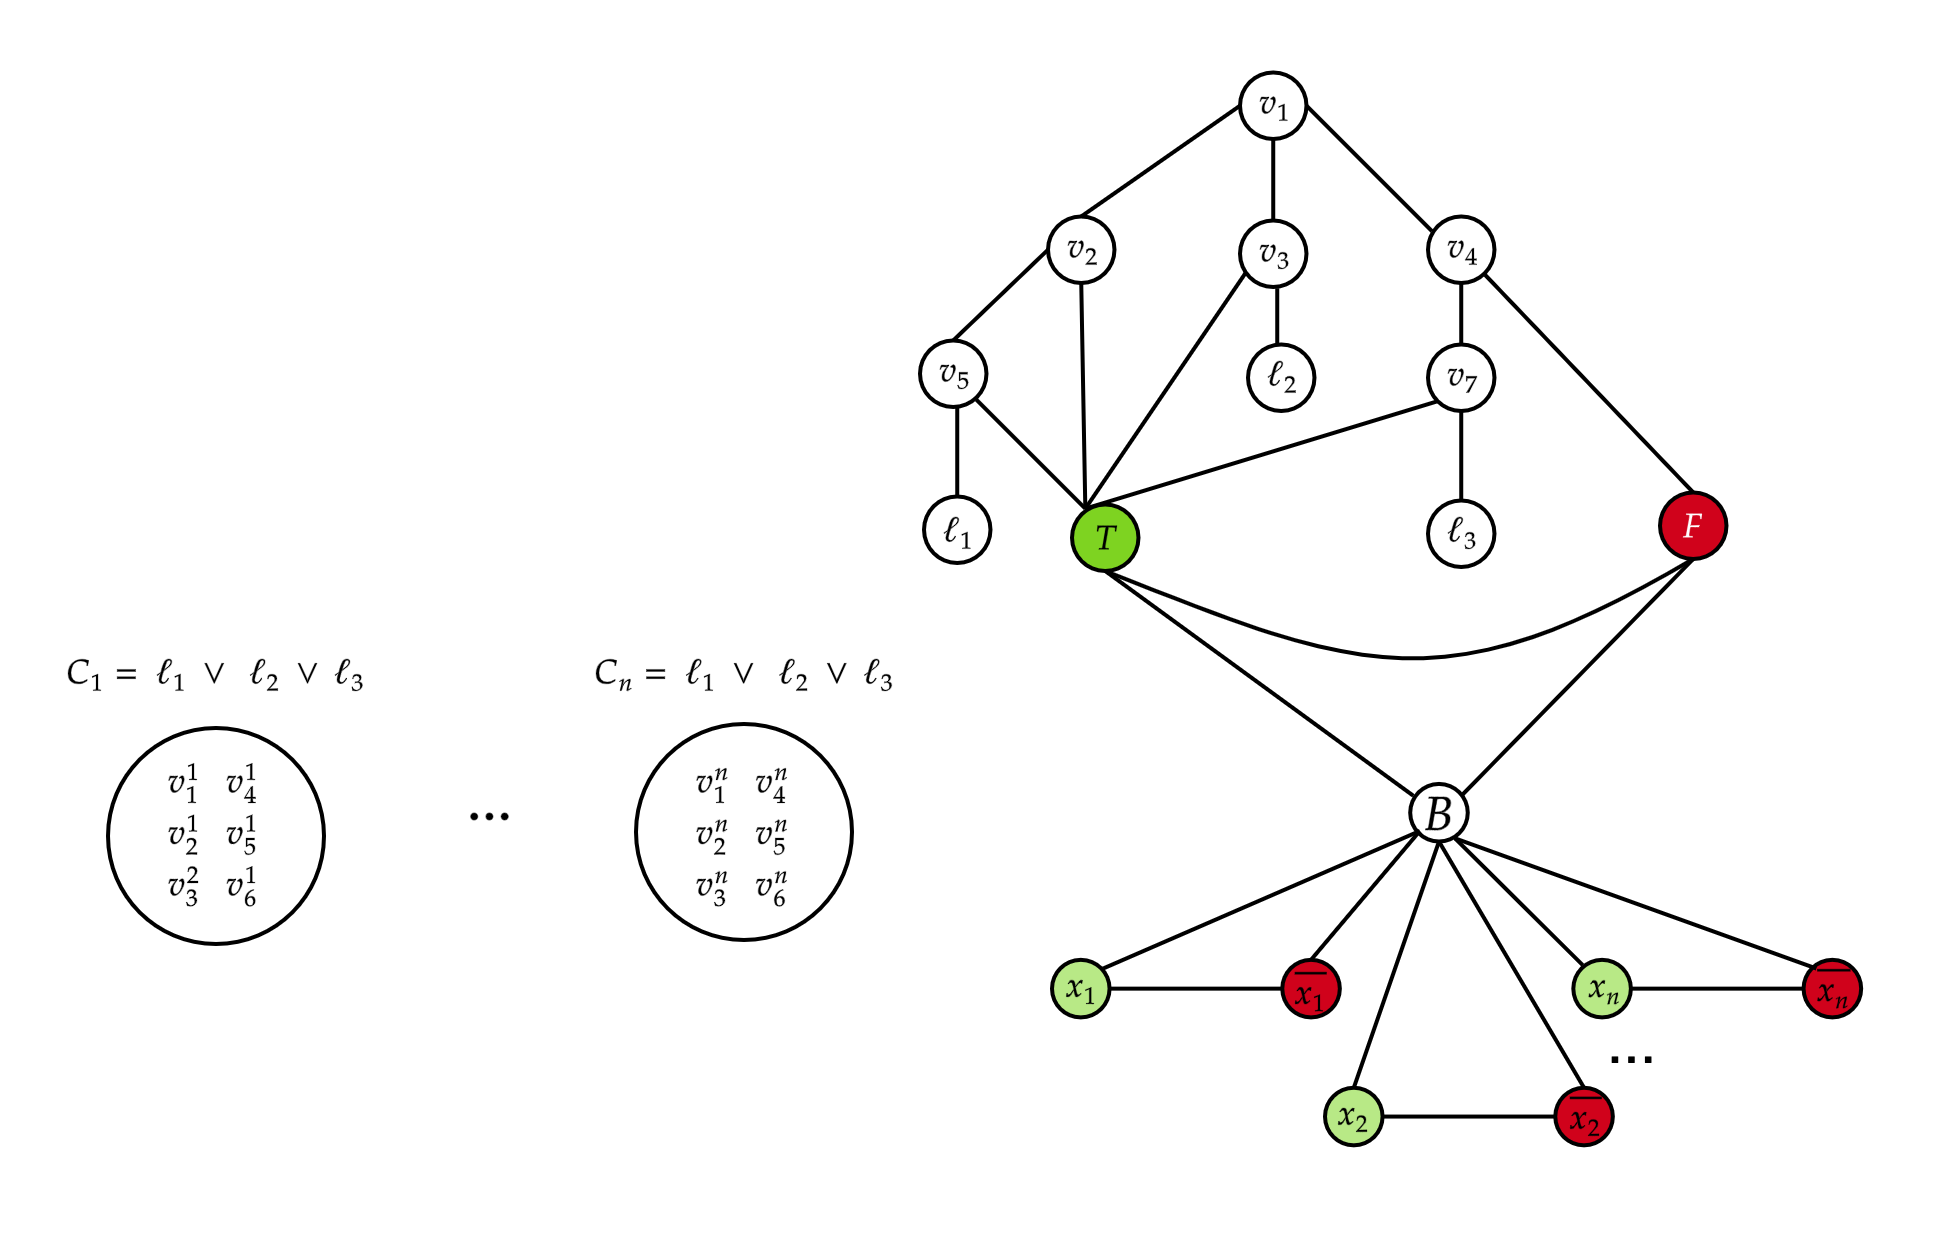
\includegraphics[width=\textwidth]{fig-18.png}
 			\end{center}

 			\item The clause for $C$ is $\ell_1 \lor \ell_2 \lor \ell_3$. We can check coloring for,
 			\begin{align*}
 				&\text{Case 1. $(\ell_1 = F, \ell_2 = F, \ell_3 = T)$} \\
 				&\text{Case 2. $(\ell_1 = F, \ell_2 = T, \ell_3 = F)$} \\
 				&\cdots \\
 				&\text{Case 8. $(\ell_1 = F, \ell_2 = F, \ell_3 = F)$}
 			\end{align*}
 			\item We discover that Case 8 cannot be colored validly, so $G$ can be 3-coloured if and only if $\texttt{I}$ is satisfiable. This completes the polynomial reduction 3-SAT $\leadsto$ 3-Colouring
 		\end{itemize}
 	\end{ex}

 	\begin{defn}[Prime Factorization Problem]
 		Given integers $N$ and $k$, we want to determine if $N$ has a prime factor $\leq k$.
 	\end{defn}

 	\begin{marginfigure}
 		The \texttt{YES} instance for prime factorization works because even if $p$ is not prime, it has some prime factorization.
 	\end{marginfigure}

 	\begin{ex}{Prime Factorization}{label}
 		We believe that prime factorization is in $NP \cap coNP - P$.
 		\begin{itemize}
 			\item Prime factorization is in NP
 			\begin{itemize}
 				\item (\texttt{YES} Instance) Give an integer $p \leq k$ such that $p |N$. 
 			\end{itemize}
 			\item Prime factorization is in coNP
 			\begin{itemize}
 				\item (\texttt{NO} Instance) Given the unique prime factorization $N = p_1p_2 \cdots p_n$, we verify that each $p_i > k$ and confirm that $p_i$ is prime in polynomial time
 			\end{itemize}
 		\end{itemize}
 	\end{ex}

 	\begin{marginfigure}
 		\textbf{Well-Known NP Complete Problems:}
 		\begin{itemize}
 			\item (Hamiltonial Cycle Problem) Given $G = (V, E)$, we want to determine if $G$ contains a cycle that uses every vertex exactly once
 			\item (Hamiltonian Path Problem) Given $G = (V, E)$, we want to determine if $G$ contains a path that uses every vertex exactly once
 			\item (Partition Problem) Given integers $x_1, \cdots, x_n \geq 0$, we want to determine if $\exists$ a subset $S \subseteq [n]$ s.t.,
 			\[\sum_{i \in S} x_i = \sum_{i \not\in S} x_i\]
 			\item (Maximum Cut Problem) Given $G = (V, E)$ and an integer $k$, we want to determine if $G$ contains a cut $\delta(S)$  containing at least $k$ edges
 		\end{itemize}
 	\end{marginfigure}

 	\begin{ex}{Taxonomy of Easy and Hard Problems}{label}
 		\resizebox{\textwidth}{!}{
 		\begin{tabular}{ll}
 		\textbf{Easy Problems}		 & \textbf{Hard Problems}	      \\ \hline
		Minimum Cut                & Maximum Cut                  \\ 
		Euler Circuit              & Hamiltonian Cycle            \\ 
		2-SAT                      & 3-SAT                        \\ 
		2-Coloring                 & 3-Coloring                   \\ 
		Shortest Path              & Longest Path                 \\ 
		Shortest Even $(s-t)$ Path & Shortest Even $(s-t)$ Dipath \\ 
		Linear Programming         & Integer Programming          \\ 
		\end{tabular}}
 	\end{ex}

 	\begin{ex}{Taxonomy of Hard Problems}{label}
 		\begin{tabular}{ll}
 		\textbf{Group} & \textbf{Example} \\ \hline
 		Packing Problems
 				& \tabitem Independent Set \\
 				& \tabitem Clique \\
 				& \tabitem Set Packing \\ \hline
			
 		Covering Problems
 				& \tabitem Vertex Cover \\
 				& \tabitem Set Cover \\ \hline

 		Partitioning Problems
 				& \tabitem 3-Coloring \\
 				& \tabitem 3D-Matching \\
 				& \tabitem Maximum Cut \\ \hline

 		Sequencing Problems
 				& \tabitem Hamiltonian Path \\
 				& \tabitem Travelling Salesman \\ \hline

 		Numerical Problems
 				& \tabitem Partition \\
 				& \tabitem Knapsack \\ \hline
		\end{tabular}
 	\end{ex}

 	\begin{ex}{Integer Programming}{label}
 		We are given an integer problem and an integer $k$. We want to determine if there is a feasible solution with value at least $k$. The minimization case is analogous. 
 	\end{ex}

 	\subsection{PSpace and Complexity Classes}
 	\begin{defn}[Exp]
 		The class \textbf{Exp} is the set of decision problems that can be solved in exponential time by a deterministic computer.
 	\end{defn}

 	\begin{defn}[NExp]
 		The class \textbf{NExp} is the set of decision problems that can be solved in exponential time by a non-deterministic computer\footnote{
 		Equivalently, this is the set of decision problems whose \texttt{YES} instances can be verified in exponential time.}.
 	\end{defn}

 	\begin{defn}[PSpace]
 		The class \textbf{PSpace} is the set of decision problems that can be solved by an algorithm using polynomial space\footnote{$P \subseteq PSpace$ since a problem that requires polynomial time uses a polynomial amount of space.}.
 	\end{defn}

 	\begin{defn}[PSpace Complete]
 		A problem $R$ is \textbf{PSpace Complete} if for every $Q \in PSpace$, there is a polynomial space reduction from $Q$ to $R$.
 	\end{defn}

 	 \begin{defn}[ExpSpace]
 		The class \textbf{ExpSpace} is the set of decision problems that can be solved by an algorithm using exponential space.
 	\end{defn}

 	\begin{thm}
 		NP $\subseteq$ PSpace.
 	\end{thm}

 	\begin{proof}
 		\noindent It suffices to show that 3-SAT $\in$ PSpace since there exists a polynomial reduction for any problem $Q \in NP$ such that $Q \leadsto$ 3-SAT. This reduction necessarily uses a polynomial amount of space. Take an instance \texttt{I} of 3-SAT. Let each binary string $b_1b_2 \cdots b_n$ of length $n$ encode a \texttt{True}/\texttt{False} assignment of the variables.
 		\[b_i = \begin{cases}
 			1 & x_i = \texttt{True} \\
 			0 & \bar{x_i} = \texttt{True}
 		\end{cases}\]

 		\begin{algorithm}
	  \caption{3SAT $\in$ PSpace}\label{3Sat}
	  \Comment{Initialize $b$ to be the $0$ vector.}
	  \Function{3SAT($b, \texttt{I}$)}{
	    \ForEach{$b \in C(\texttt{I})$}{
		    	\If{$b \text{ does not satisfy \texttt{I}}$}{
		    	\Comment{Increase $b_n$ by $1$.}
		    		$b \assign b + 1$\;
		      }
		    	\Else{
		    	  \Return{$b$}\;}
		     	}
	     	}
	\label{3satalgo}
	\end{algorithm}

 	\noindent Algorithm \ref{3satalgo} either finds a satisfying assignment, or it confirms that $\texttt{I}$ is not satisfiable. It runs in exponential time by counting to $2^n$, but it only uses a polynomial amount of space.
 	\end{proof}

 	\begin{rmk}
 		If $Q \in$ PSpace, then $Q^c \in$ PSpace. Thus, $coNP \subseteq$ PSpace.
 	\end{rmk}

 	\begin{rmk}
		It has been conjectured that,
		\[\mathbf{P} \subseteq \mathbf{N P} \subseteq \mathbf{P S P A C E} \subseteq \mathbf{E X P} \subseteq \mathbf{N E X P} \subseteq \mathbf{E X P S P A C E}\]
	\end{rmk}

 	\begin{defn}[Q-Satisfiability]
		\textbf{Q-satisfiability} is a special case of the satisfiability problem, where every clause alternates between $\forall$ and $\exists$.
		\[\text{e.g., }\exists x_{1} \forall x_{2} \exists x_{3} \forall x_{4} \cdots \quad C_{1} \wedge C_{2} \wedge \cdots \wedge C_{m}\]
	\end{defn}

	\begin{marginfigure}
		The mix of universal and existential quantifiers arises commonly in games,
		\begin{align*}
			&\exists \text{ a move such that,} \\
			&\forall \text{ moves by the opponent,} \\
			&\text{etc}.
		\end{align*}
	\end{marginfigure}

	\begin{ex}{QSat $\in$ PSpace}{label}
		Let $\phi(x_1, x_2, \cdots, x_n) = C_1 \land C_2 \land \cdots C_m$ and consider,
		\[\exists x_{1} \forall x_{2} \exists x_{3} \forall x_{4} \cdots \Phi\left(x_{1}, x_{2}, \ldots, x_{n}\right)\]

		We want to solve the assignment recursively. At step $i$,
		\[x_1 = \ell_1, \quad x_2 = \ell_2  \quad \cdots \quad x_{i-1} = \ell_{i-1}\]

		\textbf{Case 1.} $i$ is odd.
		$x_i$ is associated with $\exists$. We want,
		\[\Phi\left(\ell_{1}, \ldots, \ell_{i-1}, x_{i}, x_{i+1}, \ldots, x_{n}\right)=1\]
		for $\ell_{1}, \ldots, \ell_{i-1}$ fixed. This is true if and only if,
		\[\Phi\left(\ell_{1}, \ldots, \ell_{i-1}, 0, x_{i+1}, \ldots, x_{n}\right)=1\]
		\[\text{or}\]
		\[\Phi\left(\ell_{1}, \ldots, \ell_{i-1}, 1, x_{i+1}, \ldots, x_{n}\right)=1\]

		\textbf{Case 2.} $i$ is even.
		$x_i$ is associated with $\forall$. We want,
		\[\Phi\left(\ell_{1}, \ldots, \ell_{i-1}, x_{i}, x_{i+1}, \ldots, x_{n}\right)=1\]
		for $\ell_{1}, \ldots, \ell_{i-1}$ fixed. This is true if and only if,
		\[\Phi\left(\ell_{1}, \ldots, \ell_{i-1}, 0, x_{i+1}, \ldots, x_{n}\right)=1\]
		\[\text{and}\]
		\[\Phi\left(\ell_{1}, \ldots, \ell_{i-1}, 1, x_{i+1}, \ldots, x_{n}\right)=1\]


		\textbf{Time Complexity:}

		To solve $\phi(x_1, x_2, \cdots, x_n)$, we solve 2 subproblems,
		\[T(n) \leq 2 \cdot \underbrace{T(n-1)}_{\text{$x_n$ is fixed}} + \text{poly}(n,m)\]
		for $n$ variables and $m$ clauses.

		\vphantom{.}

		\textbf{Space Complexity:}

		We can re-use space for each subproblem.
		\begin{itemize}
			\item Solve the case $x_1 = 0$
			\item Save the solution $\phi(0, x_2, \cdots, x_n) = 0$ or $\phi(0, x_2, \cdots, x_n) = 1$
			\item Delete all other memory and reuse the space to solve $x_1 = 1$
		\end{itemize}
		This gives the space complexity,
		\[S(n) \leq S(n-1) + \text{poly}(n,m)\]
	\end{ex}

	\begin{defn}[2Exp]
		The class \textbf{2Exp} is the set of decision problems that can be solved in double exponential time, $2^{2^{\text{poly}(n)}}$ by a deterministic computer. Similar definitions exist for \textbf{2NExp} and \textbf{2ExpSpace}.
	\end{defn}

	\begin{thm}[Time and Space Hierarchy] We know that,
		\begin{itemize}
			\item Time Hierarchy Theorem I
			\[\mathbf{P} \subset \mathbf{E X P} \subset 2 \mathbf{E X P} \subset \mathbf{3 E X P} \subset \cdots\]
			\item Time Hierarchy Theorem II
			\[\mathbf{N P} \subset \mathbf{N E X P} \subset \mathbf{2 N E X P} \subset \mathbf{3 N E X P} \subset \cdots\]
			\item Space Hierarchy Theorem
			\[\mathbf{PSPACE} \subset \mathbf{EXPSPACE} \subset \mathbf{2 E X P S P A C E} \subset \cdots\]
		\end{itemize}
	\end{thm}

	\subsection{Search and Decision Problems}
	\begin{defn}[NP Hard]
		A problem $R$ is \textbf{NP Hard}\footnote{An NP Hard problem may not be in NP. For example $QSAT$ is NP Hard. In fact, it may not even be a decision problem, e.g., "Satisfy as many clauses as possible" is an optimization problem.} if for every $Q \in NP$, there is a polynomial time reduction from $Q$ to $R$.
	\end{defn}

	\begin{marginfigure}
		The optimization version of an NP Complete problem is NP Hard.
	\end{marginfigure}

	\begin{defn}[Max-SAT]
		Given a set of clauses,
		\[C_1, \cdots, C_m\]
		\noindent we need to find a \texttt{True}/\texttt{False} assignment of the variables $x_1, \cdots, x_n$ that maximizes the number of satisfied clauses.
 	\end{defn}

 	\begin{defn}[FNP]
 		Unlike a decision problem, a \textbf{search problem} requires a solution. The search analogue of NP is \textbf{FNP} (Functional Nondeterministic Polynomial Time). Given $x$ and a polynomial predicate $f(x,y)$, output $y$ such that $f(x,y)$ is \texttt{True} if $y$ exists.
 	\end{defn}

 	\begin{defn}[TFNP]
 		The class \textbf{TFNP} is the subset of problems (called "total") in FNP for which a solution is known to exist.
 	\end{defn}

 	\begin{defn}[PLS]
 		The class \textbf{PLS} is the set of total search problems that can be solved in exponential time by best-response dynamics.
 	\end{defn}

 	\begin{defn}[PPAD]
 		The class \textbf{PPAD} is the set of total search problems that can be solved in exponential time by path traversal.
 	\end{defn}

 	\begin{marginfigure}
 		\textbf{Note: } No PPAD problem is FNP Complete unless NP = coNP.
 	\end{marginfigure}

 	\begin{defn}[GD]
 		The class \textbf{GD} is the set of total search problems that can be solved approximately in exponential time by gradient descent.
 	\end{defn}

 	\begin{marginfigure}
 		\textbf{Note: } $GD = PLS \cap PPAD$.
 	\end{marginfigure}

\section{Heuristic Algorithms}
  \subsection{Backtracking and Branch-and-Bound}
Backtracking algorithms search the exponential state space of solutions using a depth-first search tree. Within this tree, interior nodes correspond to partial solutions, and leaf nodes correspond to complete solutions. Every node of the tree is labelled,
\begin{enumerate}
	\item Success, if the partial solution can be extended to a \texttt{YES} solution
	\item Failure, if the partial solution cannot be extended to a \texttt{YES} solution
	\item Active, if the partial solution is indeterminate
\end{enumerate}
In the case of a success, the algorithm outputs the solution. In the case of a failure, the algorithm backtracks. In the case of an active label, the algorithm continues searching and pruning the tree.

\begin{marginfigure}
	2-SAT is solvable in polynomial time by the backtracking heuristic, but backtracking can take exponential time to solve an instance of SAT.
\end{marginfigure}

 \begin{defn}[Backtracking]
 	The \textbf{backtracking} procedure is,
 	\begin{algorithm}
	  \caption{Backtracking Procedure}\label{backtracking}
	  \Comment{Start with some problem $P_0$}
	  \Function{Backtrack($P_0$)}{
	  	\Comment{Initialize the set of active problems}
	  	$S \assign \{P_0\}$\;
	  	\While{$S \neq \emptyset$}{
	  		\Comment{Choose a subproblem $P \in S$, expand it into smaller subproblems, and remove $P$ from $S$}
	  		$P \assign P = \{P_1, P_2, \cdots P_k\} \in S$\;
	  		\ForEach{$P_i \in P$}{
	  		\If{$(P_i) = \texttt{Success}$}{
		    	 \Return{$P_i$}\;
		      } \If{$(P_i) = \texttt{Failure}$}{
		      \Comment{Discard $P_i$}
		      $P \assign P - P_i$\;
		      } \Else{
		      \Comment{$P_i$ is indeterminate}
		      $S \assign S + P_i$\;
		      }
	  		}
	  	}
	  }
\end{algorithm}
\end{defn}

The basic approach of backtracking can be extended to optimization problems via the branch-and-bound method. A node is either,
\begin{enumerate}
	\item Infeasible, if there are no feasible completions of a partial solution
	\item Sub-Optimal, if there are feasible completions of the partial solution but they are worse than the optimal solution\footnote{To show that a subtree is sup-optimal, we need a feasible solution to compare it against. Typically, Branch-and-Bound will use Depth-First Search to find an initial feasible solution.}
	\item Feasible, if there are feasible completions to the partial solution and we know the value of the best completion
	\item Active, if the partial solution is indeterminate\footnote{\textbf{Example:} Typically, we branch on the variable that is the most fractional in the linear programming relaxation.}
\end{enumerate}

\begin{defn}[Branch-and-Bound]
	Suppose that we have a minimization problem. Each subproblem will be eliminated if the lower bound on its cost exceeds that of some other solution that we have already encountered. The \textbf{branch-and-bound} procedure is,
 	\begin{algorithm}
	  \caption{Branch-and-Bound Procedure}\label{branchbound}
	  \Comment{Start with some problem $P_0$}
	  \Function{BranchBound($P_0$)}{
	  	\Comment{Initialize the set of active problems}
	  	$S \assign \{P_0\}$\;
	  	\texttt{bestSoFar} $\assign \infty$\;
	  	\While{$S \neq \emptyset$}{
	  		\Comment{Choose a subproblem $P \in S$, expand it into smaller subproblems, and remove $P$ from $S$}
	  		$P \assign P = \{P_1, P_2, \cdots P_k\} \in S$\;
	  		\ForEach{$P_i \in P$}{
	  		\If{$(P_i) = \texttt{Success}$}{
		    	 \Comment{Update best\_so\_far}
		    	 \texttt{bestSoFar} $\assign C(P_i)$\;
		      } \If{$L(P_i) <$ \texttt{bestSoFar}}{
		      \Comment{Lower bound of $P_i$ is less than \texttt{bestSoFar}}
		      $S \assign S + P_i$\;
		      }
	  		}
	  	}
	  }
\end{algorithm}
\end{defn}

We will see an example of the Branch-and-Bound Procedure applied to the Knapsack Problem. First, we will use three facts that were proven in the context of linear programming. These are,

\begin{rmk}
	The inear programming relaxation of an integer programming problem removes the integrality constraint of each variable,
	\begin{multicols}{2}
	$\max \sum_{i=1}^{n} v_{i} \cdot x_{i}$

	s.t. $\sum_{i=1}^{n} w_{i} \cdot x_{i} \leq W$

	$\underbrace{x_{i} \in\{0,1\}}_{x_i \in \mathbb{Z^+}} \quad \forall i \in[n]$

	$\max \sum_{i=1}^{n} v_{i} \cdot x_{i}$

	s.t. $\sum_{i=1}^{n} w_{i} \cdot x_{i} \leq W$

	$\underbrace{0 \leq x_{i} \leq 1}_{x_i \in \mathbb{R^+}} \quad \forall i \in[n]$
	\end{multicols}
\end{rmk}

\begin{cor}
	The feasible region of the relaxed linear program is larger than the feasible region of the original integer linear program\footnote{The feasible region of the linear program allows for fractional solutions.}.
\end{cor}

\begin{cor}
	If the linear program is infeasible, then the integer program is infeasible. Conversely, if the linear program is feasible, then its value is at least as large as the value of the integer program by the previous corollary.
\end{cor}

\begin{ex}{Branch-and-Bound with Knapsack}{label}
	Suppose that a thief has a bag with capacity $W$. There are $n$ items to steal, and each item has an associated value $v_i$ and weight $w_i$. The thief wants to steal the subset of items of \textbf{maximum total value} that fit into the knapsack,
 	\[\begin{array}{ll}
		\operatorname{maximize} & \sum_{i=1}^{n} v_{i} \cdot x_{i} \\
		\text{ subject to } & \sum_{i=1}^{n} w_{i} \cdot x_{i} \leq W \\
		& x_{i} \in\{0,1\} \quad \forall i \in[n]
	\end{array}\]
	We can solve this via exhaustive search using a search tree \texttt{T},
	\begin{center}
		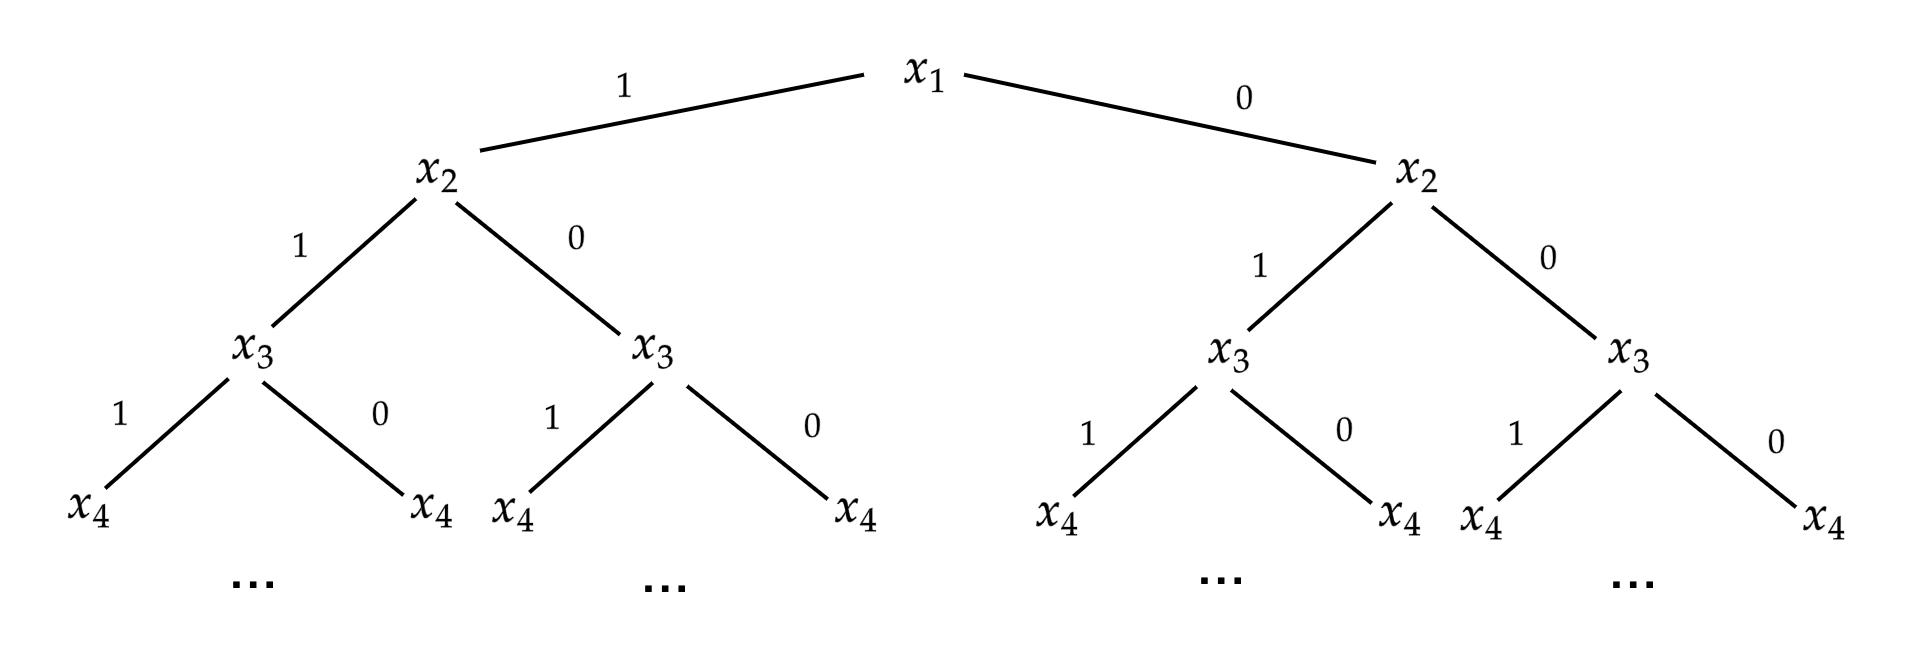
\includegraphics[width=\textwidth]{fig-19.png}
	\end{center}
	but each subtree may be of exponential size to solve. Thus, we require a method for determining if a subtree is either infeasible or worse than the optimal solution. Consider both possibilities for an assignment of \text{$x_1$}. Each decision node in the binary search tree \texttt{T} corresponds to a partial solution,
	\[\left\{x_{1}, x_{2}, x_{3}, x_{4}\right\}=\{0, *, *, *\} \quad\left\{x_{1}, x_{2}, x_{3}, x_{4}\right\}=\{1, *, *, *\}\]

	In particular, at the root of the search tree no variables have been assigned so the corresponding partial solution is empty,
	\[\left\{x_{1}, x_{2}, x_{3}, x_{4}\right\}=\{*, *, *, *\}\]

	This is useful for two reasons,
	\begin{enumerate}
		\item If the partial solution is infeasible, then every completion of the partial solution to a full solution will be infeasible.
		\item If the partial solution leads to low quality solutions, then every completion of the partial solution to a full solution will have a sub-optimal value.
	\end{enumerate}

	We can use \textbf{integer program relaxation} to,
	\begin{enumerate}
		\item Test if every completion of the partial solution is infeasible
		\item Obtain an upper bound on the value of any completion of the partial solution, which bounds the complete solution
	\end{enumerate}
	at the root of every subtree in \texttt{T}.
\end{ex}

\begin{marginfigure}
	\textbf{Solving the Knapsack Problem:}

	\noindent The Knapsack Problem can be solved quickly using a greedy algorithm:
	\begin{enumerate}
		\item Compute the value per weight $V_i := v_i / w_i$ for each item
		\item Determine the object with the maximum ratio, $x^* = \argmax_i V_i$
		\item Assign the knapsack as much of the item $x^*$ as the weight $W$ allows
		\item If the knapsack is not full, recurse on the remaining objects 
	\end{enumerate}
\end{marginfigure}

\begin{ex}{Bad Estimators with Maximum Independent Set}{label}
	Linear programs may lead to bad estimators for integer solutions. Consider the problem of finding the maximum size of an independent set on the graph $K_5$,
	\begin{center}
		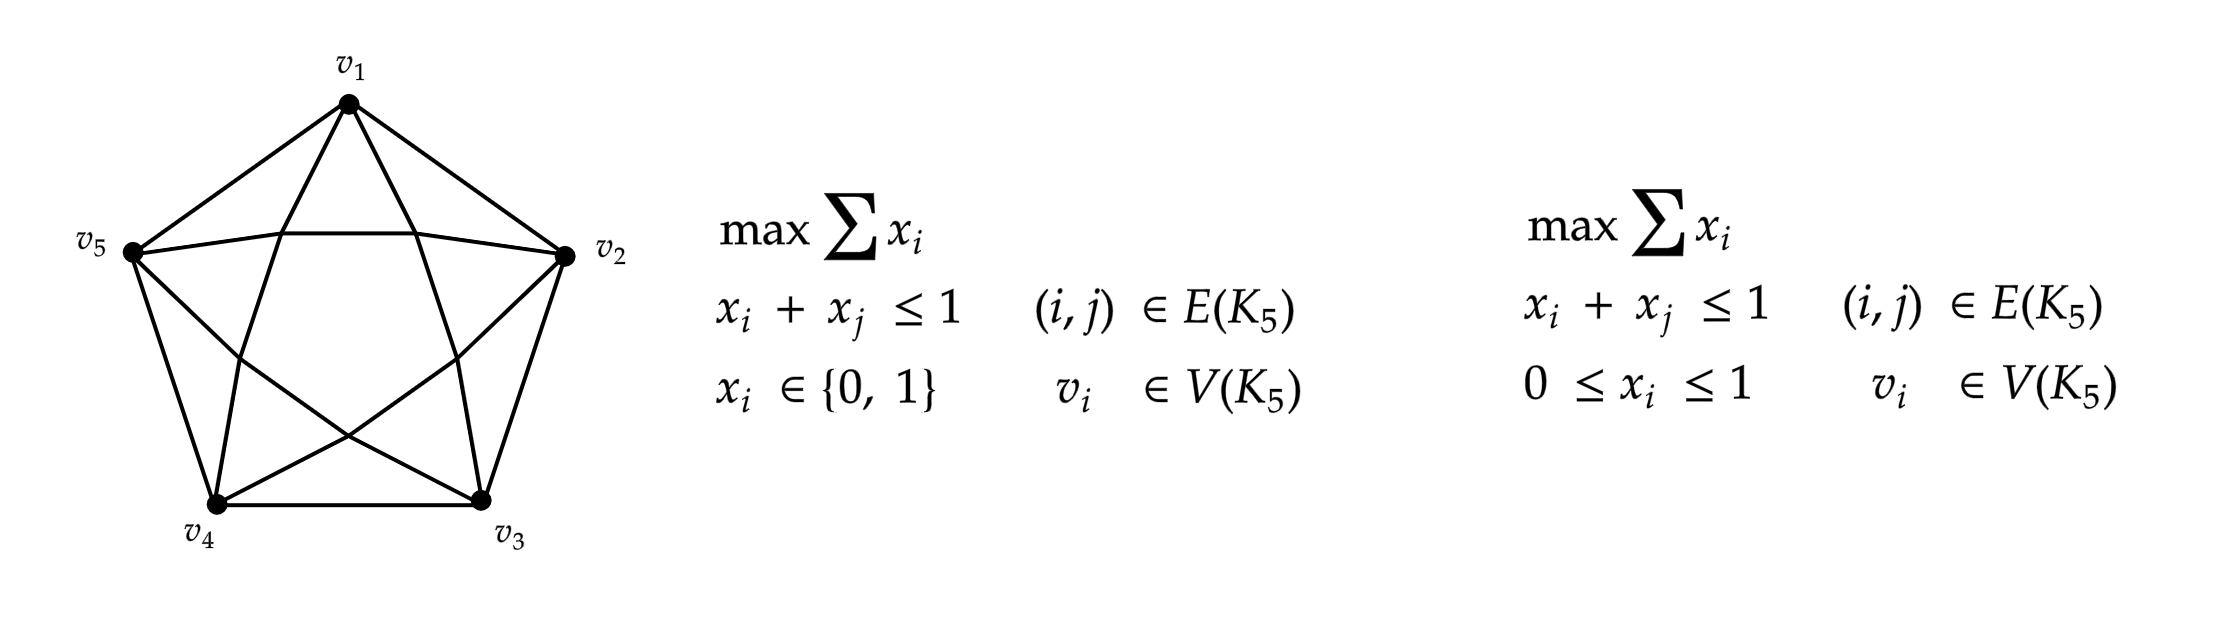
\includegraphics[width=\textwidth]{fig-20.png}
	\end{center}
	\noindent The optimal value of the linear program is $\frac{|V(G)|}{2}$, while the optimal value of the integer program is $1$. This becomes increasingly inaccurate as $|V(G)|$ grows.
\end{ex}

\noindent One possible solution is to use combinatorial estimators\footnote{See Dasgupta, Chapter 9 (p. 273)}.

\begin{ex}{Combinatorial Estimators with Salesman}{label}
	Suppose that we are given a graph \text{$G = (V, E)$} with non-negative edge costs \text{$c_e$}. The goal is to design a tour \text{$T$} that starts and ends at \text{$A$}, includes all other vertices exactly once, and has minimum total cost \text{$c(T) = \sum_e c_e$}. A partial solution \text{$Q$} is a simple path \text{$P$} with endpoints \text{$a$} and \text{$b$} passing through \text{$S \subseteq V \cup \{a,b\}$}. The corresponding subproblem is to find the best completion of the tour, that is, the cheapest complementary path from \text{$b$} to \text{$a$} with intermediate nodes \text{$V - S$}.
	\begin{center}
		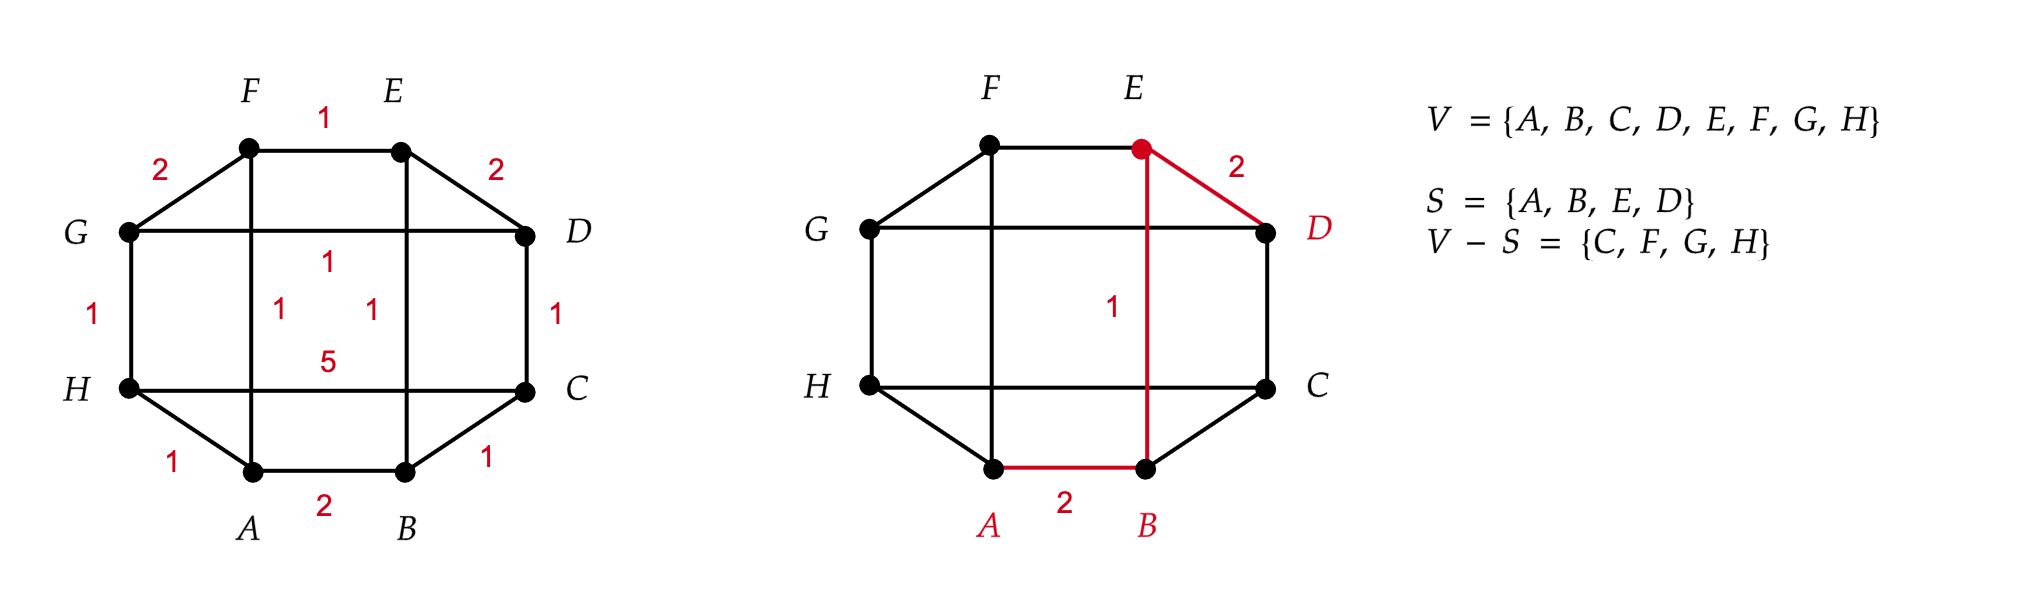
\includegraphics[width=\textwidth]{fig-21.png}
	\end{center}
	The cost of a completion is at least the sum of,
	\begin{enumerate}
		\item The lightest edge from \text{$a$} to \text{$V - S$}
		\item The lightest edge from \text{$b$} to \text{$V - S$}
		\item The minimum spanning tree of \text{$V - S$}
	\end{enumerate}
\end{ex}

\subsection{Local Search}
\begin{defn}[Local Search]
	\textbf{Local search} attempts to find a solution $S^*$ to a problem by making local improvements to the current solution $S$.
	\begin{algorithm}
	  \caption{Local Search (Minimization)}\label{localsearch}
	  \Comment{Start with some initial solution $s$}
	  \Function{LocalSearch($s$)}{
	  	\Comment{Search the neighborhood $\Gamma$ of $s$ for an alternate solution $s^{\prime}$ with a lower cost}
	  	\While{$\exists s^{\prime} \in \Gamma(s)$}{
	  		\If{$cost(s^{\prime}) < cost(s)$}{
	  			$s \assign s^{\prime}$\;
	  		}
	  	}
	  }
\end{algorithm}
\end{defn}

\begin{thm}
	Local search produces a locally optimal solution. 
\end{thm}

\begin{proof}
	We cannot return to a solution that was found previously.
\end{proof}

The neighborhood structure is imposed upon the problem, and it is a central design decision in local search. For example, an algorithm based on Local Search will run quickly with a small neighborhood. Conversely, bigger neighborhoods enable us to find a better solution.

\begin{ex}{Local Search with Maximum Cut}{label}
	In the \textbf{Maximum Cut Problem}, we are given an undirected graph \text{$G = (V, E)$} and a weight \text{$w(e)$} on each edge. We want to separate \text{$V(G)$} into two sets \text{$S$} and \text{$V - S$} so that the total weight of the edges between the two sets is as large as possible. A local improvement is a move of one vertex that produces an increase in the weight of the cut.
	\begin{align*}
		&\text{Let $\mathcal{L}=\varnothing$ and $\mathcal{R}=\mathrm{V}$} \\
		&\text{Repeat:} \\
		&\quad \text{If $\exists v \in V$ such that $\operatorname{cap}(\mathcal{L} \cup v)>\operatorname{cap}(\mathcal{L}):$} \\
		&\quad\quad \text{Set $\mathcal{L} \longleftarrow \mathcal{L} \cup v$} \\
		&\text{Else, If $\exists v \in V$ such that $\operatorname{cap}(\mathcal{L} \backslash v)>\operatorname{cap}(\mathcal{L}):$}\\
		&\quad\quad\text{Set $\mathcal{L} \leftarrow \mathcal{L} \backslash v$}
	\end{align*}

	\begin{thm}
		Any local maximum cut $\delta(\mathcal{L})$ has capacity at least half the capacity of the global maximum cut $\delta(\mathcal{L^*})$.
	\end{thm}

	\begin{proof}
		Let $\delta(\mathcal{L})$ be a local maximum cut, and let $\delta(\mathcal{L^*})$ be the global maximum cut. For any vertex $v$, let $E_v$ be the set of vertices incident to $v$. There are no local improvements for $\mathcal{L}$,
		\[\sum_{e \in E_{v} \cap \delta(\mathcal{L})} u_{e} \geq \sum_{e \in E_{v} \cap \delta(\mathcal{L})^c} u_{e}\]
		In particular, what this means is,
		\[\sum_{e \in E_{v} \cap \delta(\mathcal{L})} u_{e} \geq \frac{1}{2} \cdot \sum_{e \in E_{v}} u_{e}\]
		Therefore,
		\begin{align*}
			\operatorname{cap}(\mathcal{L})&=\frac{1}{2} \cdot \sum_{v \in V} \quad \sum_{e \in E_{v} \cap \delta(\mathcal{L})} u_{e} \\
			&\geq \frac{1}{4} \cdot \sum_{v \in V} \quad \sum_{e \in E_{v}} u_{e} \text{ plugging in the inequality} \\
			&\geq \frac{1}{2} \cdot \operatorname{cap}(\mathcal{L})
		\end{align*}
	\end{proof}
\end{ex}

\begin{marginfigure}
	\textbf{Cut Property of Minimum Spanning Trees:} Assume that edge costs are distinct. If $e$ is the cheapest edge in some cut $\delta(S)$, then $e$ must be in the minimum spanning tree.

	\begin{proof}
		Let $\mathcal{T}^*$ be a minimum spanning tree. Assume that there exists a cut $\delta(S)$ whose cheapest edge $e = (u,v)$ is not in $\mathcal{T}^*$. Since $\mathcal{T}^*$ is a spanning tree, there exists a unique path $P \subseteq \mathcal{T}^*$ from $u$ to $v$. If $\hat{e} \in P$ then $\left(\mathcal{T}^* \backslash \hat{e}\right) \cup e$ is a spanning tree. Moreover, $\hat{e} \in P \cap \delta(S)$ since $|P \cap \delta(S)|$ is odd and consequently $\geq 1$. Swapping $e$ for $\hat{e}$ results in a cheapter spanning tree than $\mathcal{T}^*$.
	\end{proof}
\end{marginfigure}

\begin{ex}{Minimum Spanning Tree Problem}{label}
	The Local Search Algorithm can be used to construct an optimal solution to the \textbf{Minimum Spanning Tree Problem}. We say that a spanning tree $\hat{T}$ is in the neighborhood of a spanning tree $T$ if they differ in exactly one edge,
	\[\Gamma(\mathcal{T})=\{\hat{\mathcal{T}}: \mathcal{T}=(\hat{\mathcal{T}} \cup e) - \hat{e} \text{ where } e \in \mathcal{T} \text{ and } \hat{e} \in \hat{\mathcal{T}}\}\]
	
	We will search for an improving swap that reduces the total cost of the spanning tree.
	\begin{align*}
		&\text{Let $\mathcal{T}$ be a spanning tree.} \\
		&\text{While $\exists \hat{\mathcal{T}} \in \Gamma(\mathcal{T})$ s.t. $c(\mathcal{\hat{T}}) < c(\mathcal{T})$}: \\
		&\quad \text{Set $\hat{\mathcal{T}} \leftarrow \mathcal{T}$}
	\end{align*}
	This outputs a locally minimum spanning tree \text{$\mathcal{T}$}, but we can show that it is in fact the globally minimum spanning tree \text{$\mathcal{T}^*$}. Assume not. If \text{$\mathcal{T} \neq \mathcal{T}^*$}, then \text{$\exists e \in \mathcal{T}^* - \mathcal{T}$}. By the Cut Property, \text{$e$} is the cheapest edge in some cut \text{$\delta(S)$}. Since \text{$\mathcal{T}$} is a spanning tree, there is a unique path $P$ in $\mathcal{T}$ from $u$ to $v$. Thus, there is an edge \text{$\hat{e} \in P \cap \delta(S) \text { with } \hat{e} \neq e$}. But then \text{$\hat{\mathcal{T}}=(\mathcal{T} \cup e) - \hat{e}$} is a cheaper spanning tree than $\mathcal{T}$.
\end{ex}

\begin{ex}{Local Search with Salesman}{label}
	A tour $\hat{\mathcal{T}}$ is said to be in the neighborhood of $\mathcal{T}$ if they differ in exactly two edges. The Local Search Algorithm looks for an improving 2-swap that reduces the cost of the tour. However, there might be an exponential number of iterations needed to solve the Travelling Salesman Problem in this way. Moreover, the final tour is only guaranteed to be locally optimal. 
\end{ex}

\section{Approximation Algorithms}
 \subsection{Bounding the Optimum}

\begin{defn}[Approximation Algorithm]
	An algorithm \texttt{A} is an \textbf{$\alpha$-approximation} ($\alpha \geq 1$) for a problem $Q$ if for every instance $I$,
	\begin{enumerate}
		\item \texttt{A} outputs a feasible solution \texttt{S}
		\item \texttt{A} runs in polynomial time
		\item If $Q$ is a minimization problem, then cost$(\texttt{S}) \leq \alpha \cdot $ cost$(\texttt{OPT})$
		\item If $Q$ is a maximization problem, then val$(\texttt{S}) \geq 1/\alpha \cdot $ val$(\texttt{OPT})$
	\end{enumerate}
\end{defn}

\subsection{Application 1: Travelling Salesman Problem}
Suppose that we are given a complete, undirected graph $K_n$ with non-negative integer costs $c$ for each edge. The goal is to find the cheapest Hamiltonian cycle of $G$.

\begin{defn}[Triangle Inequality]
	The edge-cost function $c: V(K_n) \times V(K_n) \rightarrow \mathbb{R}^+$ satisfies the \textbf{triangle inequality} if the following holds,
	\[c\underbrace{(v_1, v_2)}_{e_1} \leq c\underbrace{(v_1, v_3)}_{e_2} - c\underbrace{(v_3, v_2)}_{e_3} \quad \forall e_1, e_2, e_3 \in E(K_n)\]
\end{defn}

\begin{marginfigure}
	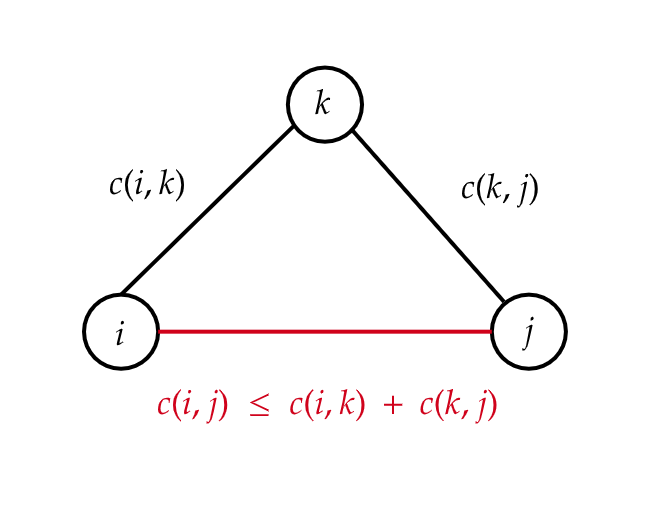
\includegraphics[width=\textwidth]{fig-22.png}
	\caption{Illustration of metric costs.}
\end{marginfigure}

\begin{defn}[Walk]
	A \textbf{walk} is a sequence of vertices,
	\[v_1, \cdots, v_n \text{ such that } (v_i, v_j) \in E(G) \text{ for all $i,j \in [n]$}\]
\end{defn}

\begin{defn}[Eulerian Graph]
	Let $G = (V, E)$ be a multigraph. $G$ is \textbf{Eulerian} if it has a closed walk that uses every edge exactly once.
\end{defn}

\begin{marginfigure}
	\begin{enumerate}
		\item A \textbf{path} is a walk with no vertex repeated, while a \textbf{trail} is a walk with no edge repeated.
		\item An \textbf{Euler trail} is a trail that uses every edge, and an \textbf{Euler tour} is a closed Euler trail.
	\end{enumerate}
\end{marginfigure}

\begin{thm}[2-Approximation TSP]
	The \texttt{TreeDoubling} algorithm is a \textbf{2-approximation algorithm} for the Metric TSP.
	\begin{algorithm}
	  \caption{2-Approximation Travelling Salesman}\label{2approxTSP}
	  \Comment{$\texttt{Prim}(G, c)$ uses Prim's Algorithm to find a minimum spanning tree in $G$, given the weight function $c$}
	  \Function{TreeDoubling($K_n$, $c$)}{
	  	\Comment{Find a minimum spanning tree $T$ of $K_n$}
	  	$T \assign \FuncCall{Prim}{$K_n$, $c$}$\;
	  	\Comment{Duplicate each edge in $T$ to obtain a Eulerian multigraph $T^{\prime}$ (all vertex degrees in $T^{\prime}$ are even)}
	  	$T^{\prime} \assign (V(K_n) \text{, } 2 \cdot E(T))$\;
		\Comment{Compute a Eulerian tour $H$ of $T^{\prime}$. Whenever a vertex $v$ is visited in $H$ that was already visited, skip $v$ and proceed with the next unvisited node along the cycle}
	  	$H \assign \FuncCall{PreOrder}{$T^*$}$\;
	  	\Comment{Return resulting Hamiltonian tour $H$}
	  	\Return{$H$}\;
	  }
	\end{algorithm}
\end{thm}

\begin{proof}
 	\texttt{TreeDoubling} is a 2-approximation algorithm if,
	\begin{enumerate}
		\item It outputs a feasible tour $H$
		\item It runs in polynomial time
		\item Its cost is at most $2 \cdot c(\texttt{OPT})$
	\end{enumerate}

	\noindent Polynomial running time is guaranteed since \texttt{Prim} runs in $O(|V(K_n)|^2)$ and \texttt{PreOrder} is a form of Depth First Search, which is in $O(|V(K_n)| + |E(K_n)|)$. Moreover, the \texttt{TreeDoubling} algorithm clearly outputs a feasible solution since $H$ is a Eulerian tour by construction.

	It remains to prove that $c(H) \leq 2 \cdot \texttt{OPT}$, where \texttt{OPT} is the optimal tour in $K_n$. Let $T$ be a minimum spanning tree of $K_n$ with respect to $c$. We know that $c(T) \leq c(\texttt{OPT})$ since deleting any edge of a Hamiltonian tour gives a spanning tree. Therefore,
	\begin{align*}
		c(H) &\leq c(2 \cdot T) \text{ by short-cutting} \\
			 &= 2 \cdot c(T) \\
			 &\leq 2 \cdot (\texttt{OPT})
	\end{align*}
	\noindent Thus, we have an approximation algorithm with $\alpha = 2$.
\end{proof}

\begin{marginfigure}
	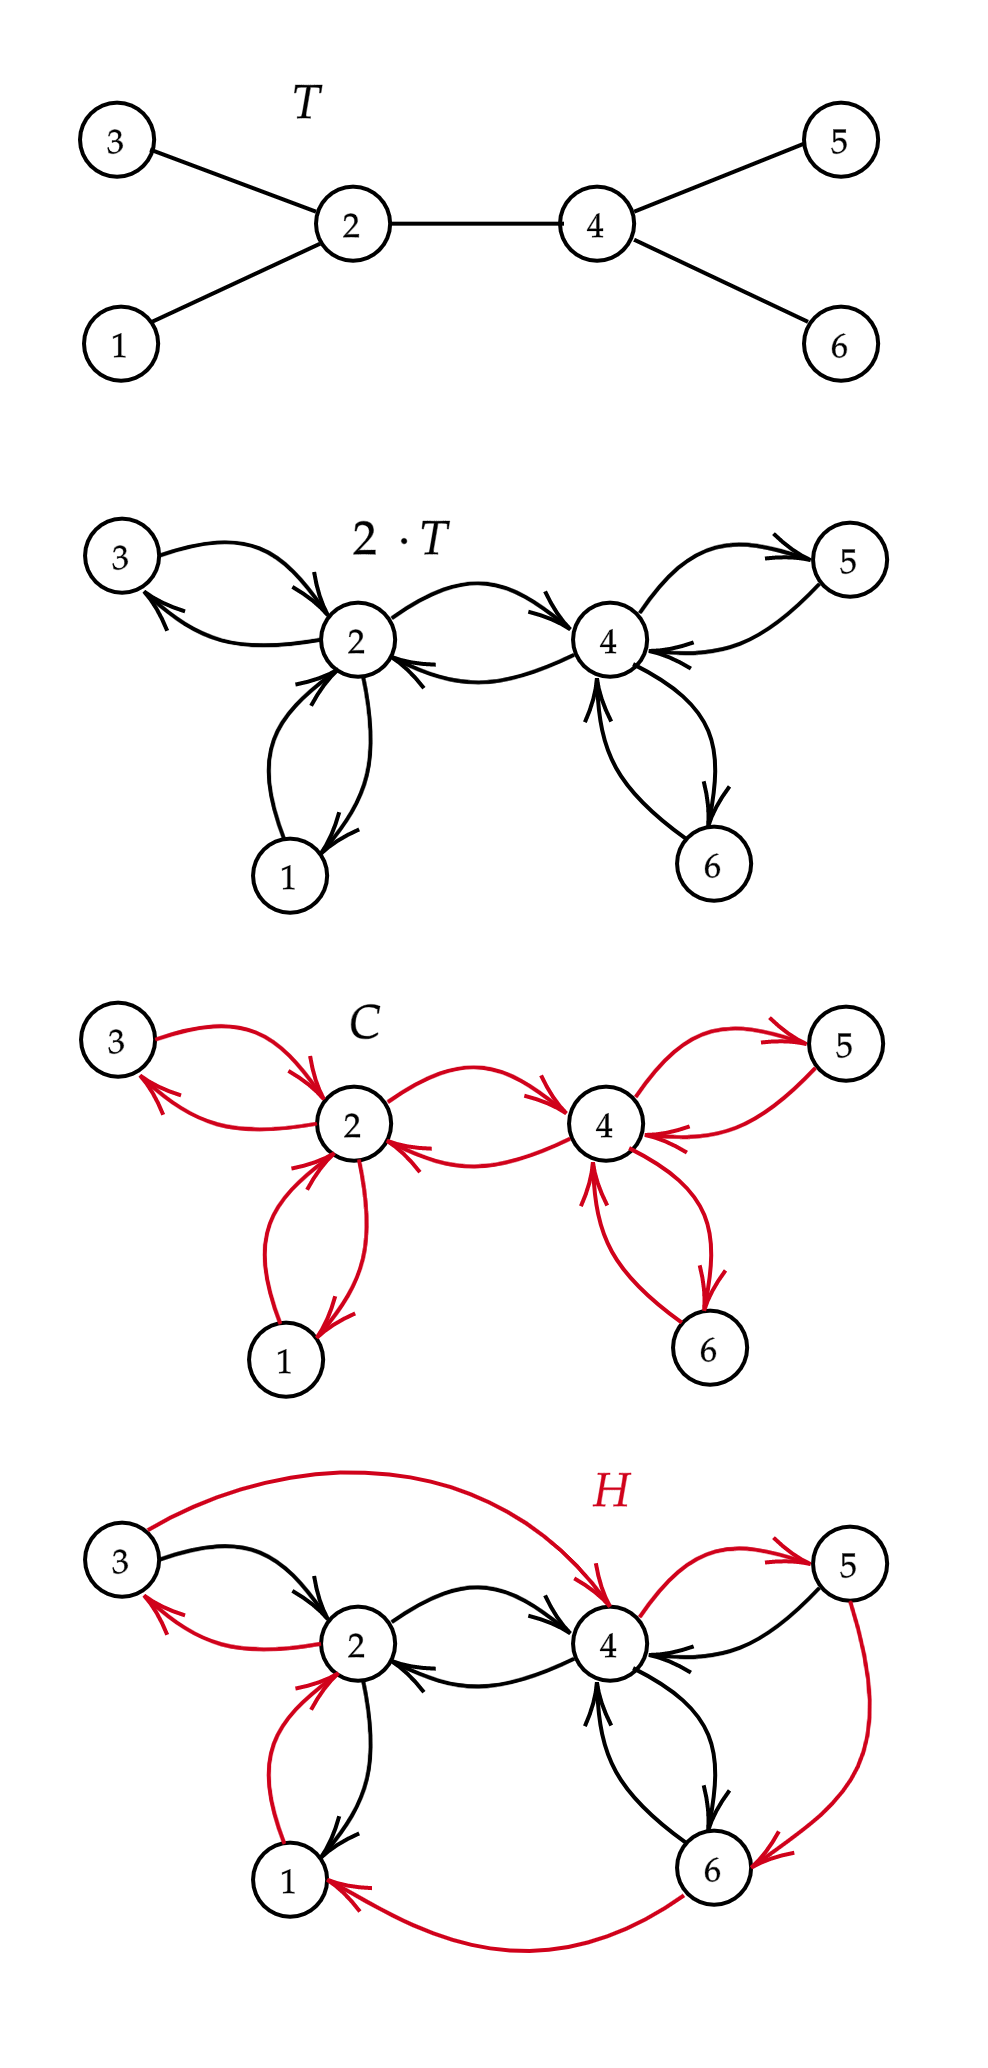
\includegraphics[width=\textwidth]{fig-23.png}
	\caption{Illustration of the \texttt{TreeDoubling} algorithm.}
\end{marginfigure}

\begin{marginfigure}
	Suppose that  $H^{\prime}$ is a lower bound for \texttt{OPT}. We can ask \textbf{four questions},
	\begin{enumerate}
		\item Is the analysis tight with respect to the lower bound for \texttt{OPT}? Find an example where $c(H) = \alpha \cdot H^{\prime}$
		\item Is the lower bound for \texttt{OPT} closer to \texttt{OPT} than a factor of 2? Find an example where $\texttt{OPT} = \alpha \cdot  H^{\prime}$
		\item Is the analysis tight with respect to \texttt{OPT}? Find an example where $c(H) = \alpha \cdot \texttt{OPT}$
		\item Is there a better approximation algorithm for our problem?
	\end{enumerate}
\end{marginfigure}

The natural question that arises is whether an approximation guarantee of $\alpha = 2$ is sufficient. There are four questions to ask,
\begin{enumerate}
	\item Is our analysis tight with respect to the lower bound $T$? Yes.
	\begin{center}
			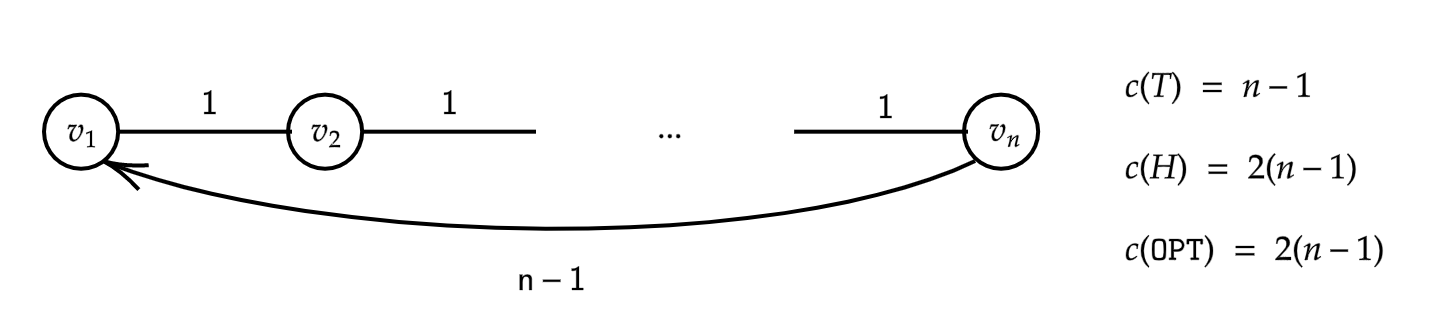
\includegraphics[width=\textwidth]{fig-24.png}
	\end{center}

	\item Is the lower bound closer to \texttt{OPT} than a factor of 2? No.
	\begin{center}
			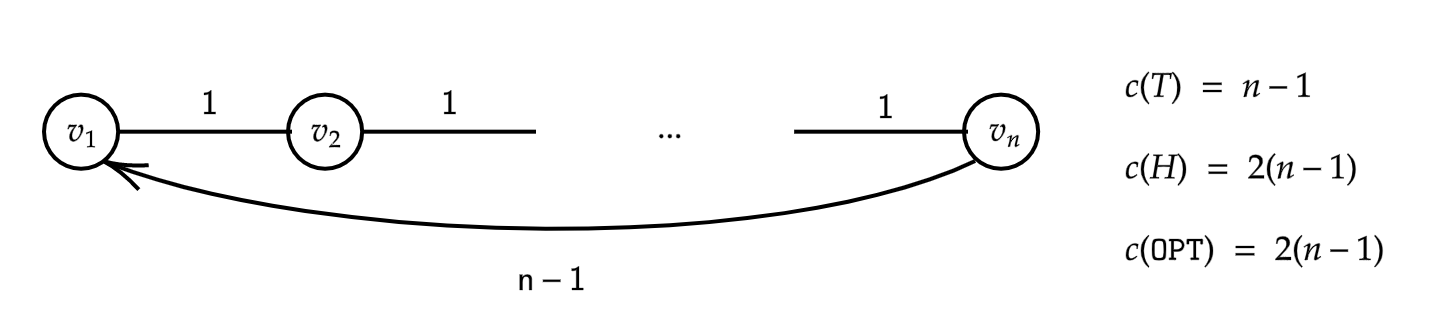
\includegraphics[width=\textwidth]{fig-24.png}
	\end{center}

	\item Is the analysis tight with respect to \texttt{OPT}? Yes.
	\begin{center}
			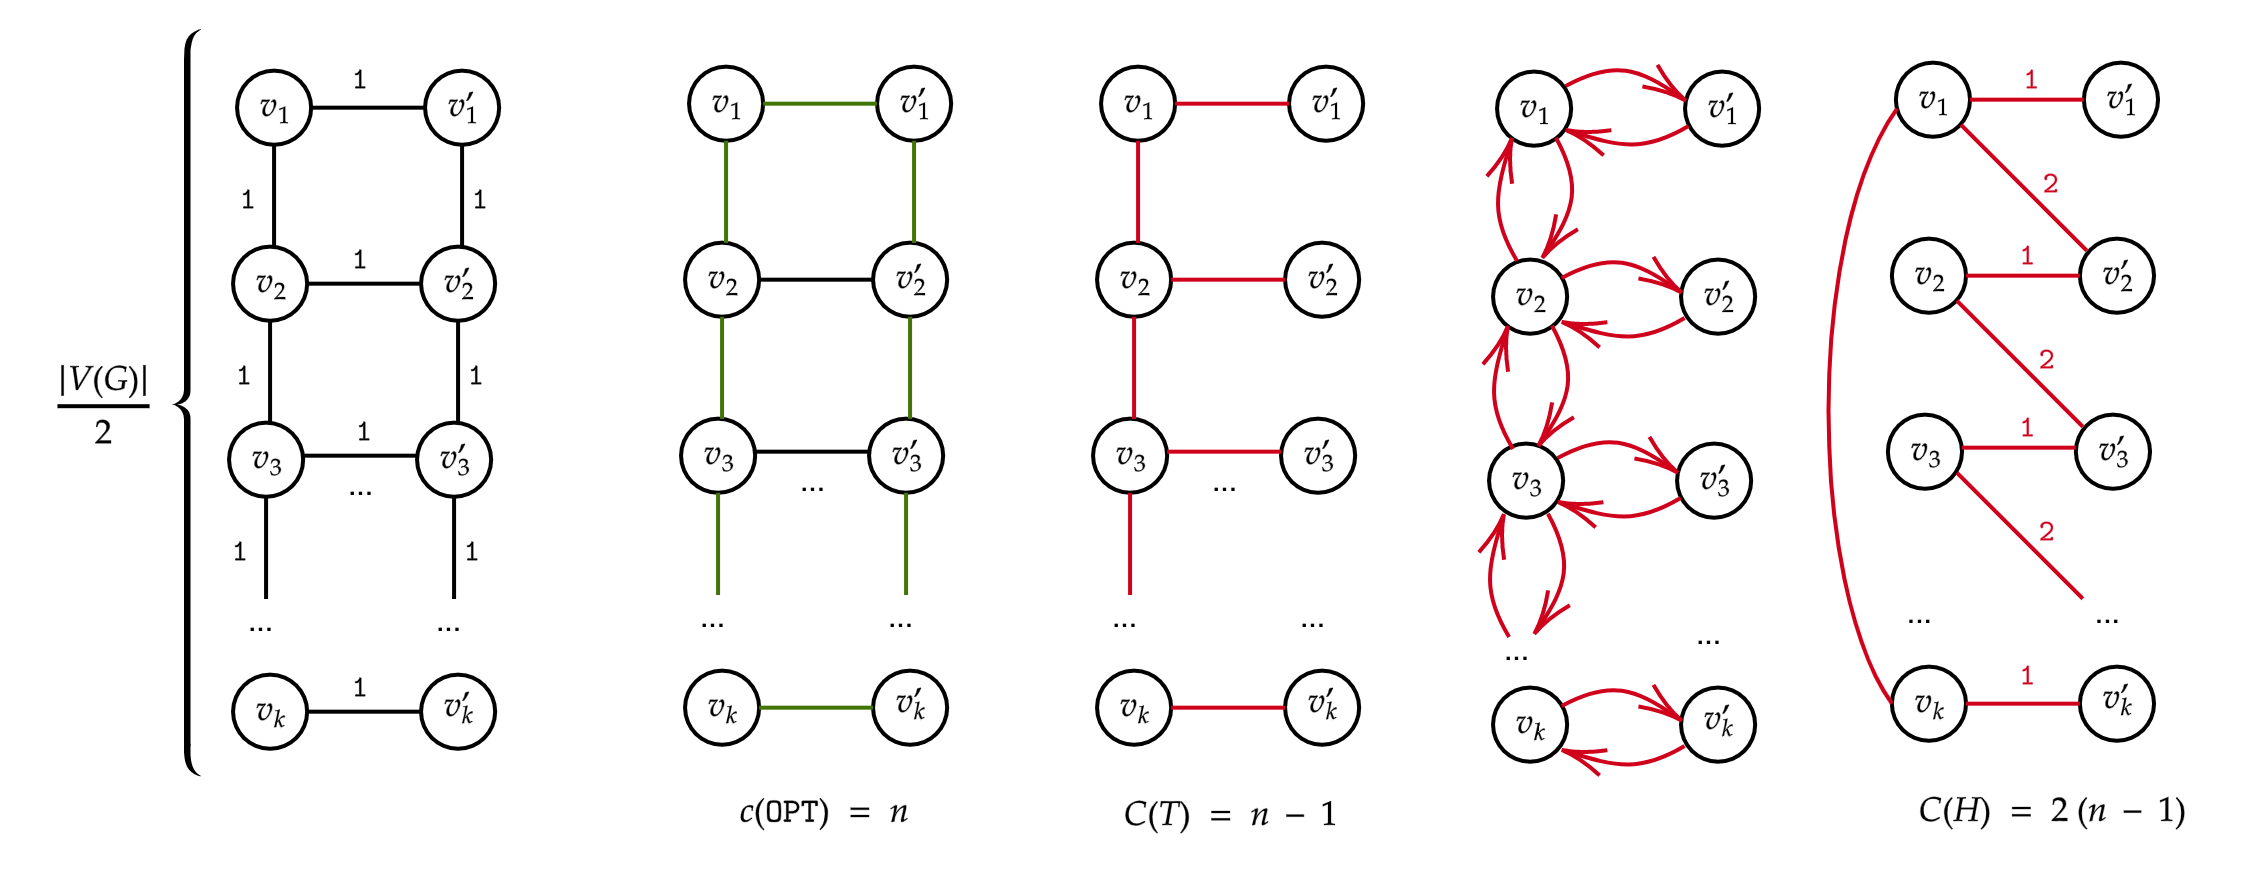
\includegraphics[width=\textwidth]{fig-25.png}
	\end{center}

	\item Is there a better approximation algorithm?
	\noindent Yes. there is a $\frac{3}{2}$-approximation algorithm for the metric TSP.
\end{enumerate}

\begin{marginfigure}
	See the following \href{https://link.springer.com/content/pdf/10.1007%2F978-0-387-30162-4_230.pdf}{paper} for more information on the Metric TSP.

\end{marginfigure}

\begin{defn}[Matching on a Set]
	A matching $M$ of $G$ is called a \textbf{matching on $U \subseteq V(G)$} if all edges of $M$ consist of two vertices from $U$\footnote{Recall that the matching is called "perfect" if every vertex of $U$ is incident with an edge of $M$.}. 
\end{defn}

\begin{thm}[3/2-Approximation TSP]
	The \texttt{Christofides} algorithm is a \textbf{3/2-approximation algorithm} for the Metric TSP\footnote{Instead of doubling the number of edges, we can add edges between odd degree vertices. The graph will still have even degree vertices and therefore an Euler tour.}.
	\begin{algorithm}
	  \caption{3/2-Approximation Travelling Salesman}\label{23approxTSP}
	  \Comment{$\texttt{Prim}(G, c)$ uses Prim's Algorithm to find a minimum spanning tree in $G$, given the weight function $c$}
	  \Function{Christofides($K_n$, $c$)}{
	  	\Comment{Find a minimum spanning tree $T$ of $K_n$}
	  	$T \assign \FuncCall{Prim}{$K_n$, $c$}$\;
	  	\Comment{Let $U \subseteq V(T)$ be the odd degree vertices in $T$}
	  	$U \assign \{v \mid v \in V(T) \text{ and deg}(v) = 2k+1\}$\;
	  	\Comment{Compute a minimum weight perfect matching $M$ on the subgraph induced by $U$}
	  	$M \assign \FuncCall{Ford-Fulkerson}{$K_n$, $U$, $c$}$\;
	  	\Comment{Compute a Eulerian tour $H$ of $T \cup M$, taking shortcuts to obtain a Hamiltonian tour}
	  	$H \assign \FuncCall{PreOrder}{$T^*$}$\;
		\Return{$H$}\;
	  }
	\end{algorithm}
\end{thm}

\begin{proof}
	\texttt{Christofides} is a 3/2-approximation algorithm if,
	\begin{enumerate}
		\item It outputs a feasible tour $H$
		\item It runs in polynomial time
		\item Its cost is at most $3/2 \cdot c(\texttt{OPT})$
	\end{enumerate}

	\noindent First observe that the number of odd degree vertices of the spanning tree $T$ is even, since the sum of the degrees of all vertices is $2(n-1)$ by the Handshaking Lemma. Thus, a perfect matching on $U$ exists. Moreover, it can be found using maximum flows in $O(n^3)$. Hence, the algorithm is polynomial. Moreover, the \texttt{Christofides} algorithm outputs a feasible solution since $H$ is a Eulerian tour by construction.

	The weight of the Eulerian tour $H$ is at most $c(T) + c(M)$, and it was proven earlier that $c(T) \leq \texttt{OPT}$\footnote{$c(H) < c(T) + c(M)$ by shortcutting and applying the triangle inequality.}. It suffices to show that $c(M) \leq \frac{1}{2} \cdot \texttt{OPT}$, where \texttt{OPT} is the optimal tour in $K_n$.

	Since \texttt{OPT} is a Hamiltonian Cycle, we can shortcut to obtain a cycle $\hat{C}$ on the set of odd degree vertices. Clearly $|\hat{C}| = |U|$, so $\hat{C}$ can be partitioned into two matchings $M_1, M_2$. In particular,
	\begin{align*}
		\frac{1}{2}\left(\texttt{OPT} \right) &= \frac{1}{2}\left(c(M_1) + c(M_2)\right) \\
											  &\geq c(M)
	\end{align*}
	\noindent since $M$ was computed to be the minimum weight perfect matching.
\end{proof}

\begin{marginfigure}
	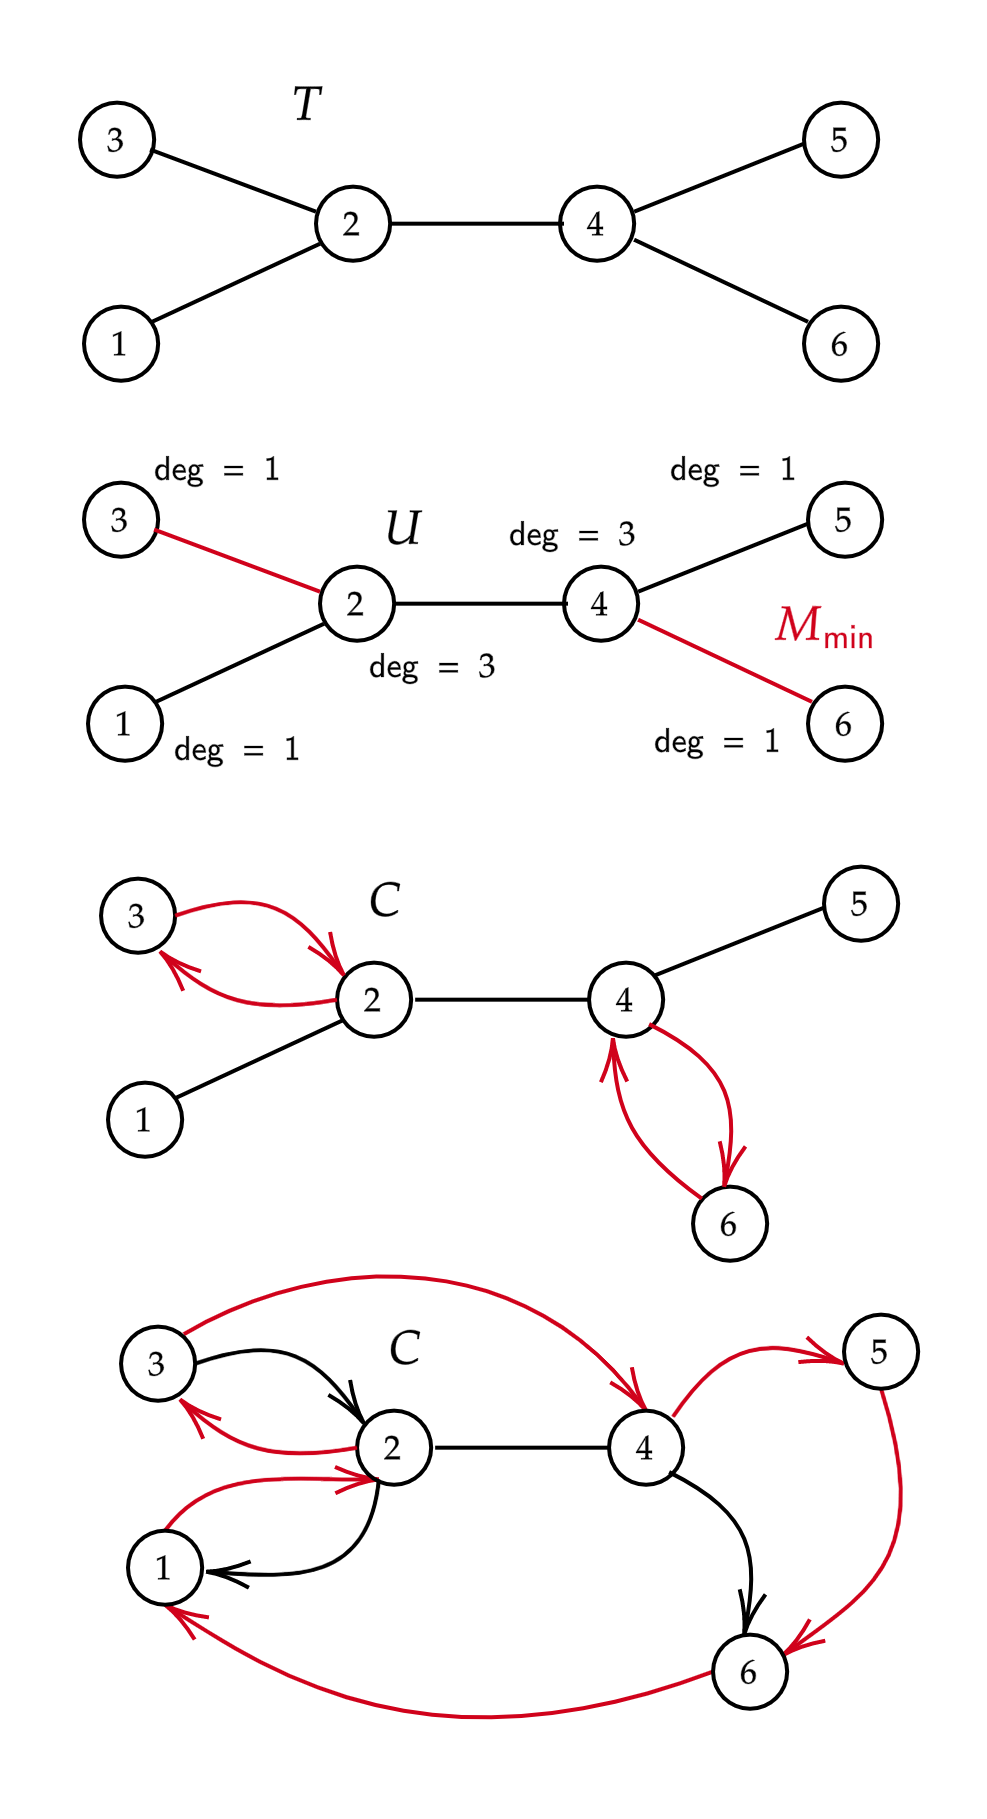
\includegraphics[width=\textwidth]{fig-28.png}
	\caption{Illustration of the \texttt{Christofides} algorithm.}
\end{marginfigure}

\begin{thm}
	There is no polynomial-time $\alpha$-approximation algorithm for the traveling salesman problem on general weighted graphs, unless $P = NP$.
\end{thm}

\begin{proof}
	Construct a cost function for $K_n$ as follows,
	\[
		c(e) := \begin{cases}
						1 & e \in E(G) \\
						\alpha \cdot n& \text{ otherwise}
				   \end{cases}
	\]
	\noindent  Suppose not. If $G$ has a Hamiltonian cycle, then its cost in $K_n$ is $n$. Any other Hamiltonian cycle has cost $\geq \alpha \cdot n + (n - 1) > \alpha n$. Thus, if $G$ has a Hamiltonian cycle, then the $\alpha$-approximation algorithm for the traveling salesman problem must find a tour in $K_n$ of cost $\leq \alpha \cdot n$. The only such tours have cost $n$, and they are Hamiltonian cycles in $G$. This means that the $\alpha$-approximation algorithm can distinguish between \texttt{YES} and \texttt{NO} instances of the Hamiltonian Cycle Problem, which is known to be an NP-complete decision problem.
\end{proof}

\subsection{Application 2: Multiway Cut}
Suppose that we are given an undirected graph \text{$G = (V, E, c)$} with non-negative edge weights $c$, and a set of terminals,
\[X = \{x_1, \cdots, x_k\} \subseteq V(G)\]

\begin{defn}[Multiway Cut]
	A \textbf{multiway cut} is a set of edges that leaves each of the terminals in a separate component\footnote{The Multiway Cut Problem is NP-complete for $k \geq 3$. When $k = 2$, this is precisely finding the minimum $(s - t)$ cut, which can be computed efficiently using \texttt{Ford-Fulkerson}.}.
\end{defn}

\begin{defn}[Multiway Cut Problem]
	The \textbf{Multiway Cut Problem} is the problem of finding a minimum weight set of edges $F \subseteq E(G)$ such that removing $F$ from $G$ separates all terminals\footnote{No connected component of $G(V, E - F)$ contains two terminals from $S$.}.
\end{defn}

\begin{thm}[2-Approximation Multiway Cut]
	The \texttt{MultiApprox} algorithm is a \textbf{2-approximation algorithm} for Multiway Cut.
	\begin{algorithm}
	  \caption{2-Approximation Multiway Cut}\label{2approxMC}
	  \Function{MultiApprox($G$, $c$)}{
	  	\ForEach{$i \in [k]$}{
	  		\Comment{Find a minimum weight cut $\delta(S_i)$ separating $x_i$ from a super-vertex $X_i := X - \{x_i\}$}
	  		$X_i \assign X - \{x_i\}$\;
	  		$C_i \assign \FuncCall{Ford-Fulkerson}{$G$, $c$, $x_i$, $X_i$}$\;
	  	}
	  	\Comment{Return the union of each cut $C_i$}
	  	$C \assign \bigcup_{i = 1}^k \delta(C_i)$\;
	  	\Return{$C$}\;
	  }
	\end{algorithm}
\end{thm}

\begin{proof}
	\texttt{MultiApprox} is a 2-approximation algorithm if,
	\begin{enumerate}
		\item It outputs a feasible cut $C$
		\item It runs in polynomial time
		\item Its cost is at most $2 \cdot \texttt{OPT}$
	\end{enumerate}

	\noindent The cut $C_i$ can be computed efficiently at each iteration by running the \texttt{Ford-Fulkerson} algorithm to find maximum flow. We call a polynomial algorithm a constant number of times, so \texttt{MultiApprox} is polynomial. Moreover, $C = \bigcup_{i = 1}^k \delta(C_i)$ is a feasible multiway cut\footnote{To see this, note that for any pair $x_i, x_j$, $\delta(S_i)$ and $\delta(S_j)$ separate $x_i$ and $x_j$.}. 

	Let \texttt{OPT} denote the optimal multiway cut in $G$. Then $G - \texttt{OPT}$ has components $T_1, \cdots, T_k$, where $x_i \in T_i$. Thus, $\texttt{OPT} = \bigcup_{i = 1}^k \delta(T_i)$ and $c(\texttt{OPT}) = \frac{1}{2} \cdot \sum_i c(\delta(T_i))$ since $e \in \texttt{OPT}$ appears in two of the $\delta(T_i)$,
	\begin{align*}
		c(\texttt{OPT}) &= \frac{1}{2} \cdot \sum_i c(\delta(T_i)) \\
						&\geq \frac{1}{2} \cdot \sum_i c(\delta(C_i)) \\
						&= \frac{1}{2} \cdot c(C) \\
	\end{align*}
	where the second last line follows by the minimality of the cut returned by \texttt{Ford-Fulkerson}, and the last line follows by the union bound. That is, an edge $e \in C$ can appear in only one $\delta(C_i)$ since $C_1 \cup \cdots \cup C_k$ need not equal $V(G)$.
\end{proof}

\subsection{Application 3: Weighted Vertex Cover}
Given a graph $G = (V, E, c)$ and non-negative costs $c$, the goal is to find a minimum cost vertex cover $S \subseteq V(G)$.

\begin{thm}
	The \texttt{GMatching} algorithm is a \textbf{2-approximation algorithm} for the Unweighted Vertex Cover Problem\footnote{The following bound can be seen to be tight by looking at the unweighted vertex cover for a star.}.
	\begin{algorithm}
	  \caption{2-Approximation Vertex Cover}\label{vertcov}
	  \Function{GMatching($G$, $c$)}{
	  	\Comment{Find a maximal cardinality matching $M$ in $G$}
	  	$M \assign \FuncCall{MaxMatching}{$G$}$\;
	  	\Comment{Output $C$, the end vertices of edges in $M$}
	  	$C \assign V(M)$\;
	  	\Return{$C$}\;
	  }
	\end{algorithm}
\end{thm}

\begin{proof}
	\texttt{GMatching} is a 2-approximation algorithm if,
	\begin{enumerate}
		\item It outputs a feasible vertex cover $C$
		\item It runs in polynomial time
		\item Its cost is at most $2 \cdot \texttt{OPT}$
	\end{enumerate}

	\noindent \texttt{GMatching} runs in polynomial time because we can find a maximal matching and its endpoints in polynomial time. Moreover, \texttt{GMatching} outputs a feasible solution because the  maximality of $M$ guarantees that $C$ is a vertex cover of $G$. Since $C^c := V - C$ is an independent set, adding any edge $(i,j) \in E(G - C)$ to $M$ creates a bigger matching.

	We need to show that $|C| \leq 2 \cdot \texttt{OPT}$. Let $C^*$ be the minimum vertex cover in $G$, so that $|C^*| = \texttt{OPT}$. Then $\texttt{OPT} \geq |M|$, where $M$ is the maximal matching in $G$. This is because $C^*$ must contain at least one endpoint of each edge in $M$. But, $|C| = 2 \cdot |M|$, so,
	\[|C| = 2 \cdot |M| \leq 2 |C^*| = 2 \cdot \texttt{OPT}\]
\end{proof}

\begin{marginfigure}
	\textbf{Recall: } A basic solution to a linear program is a feasible solution that is not a convex combination of two other feasible solutions.

	\begin{center}
		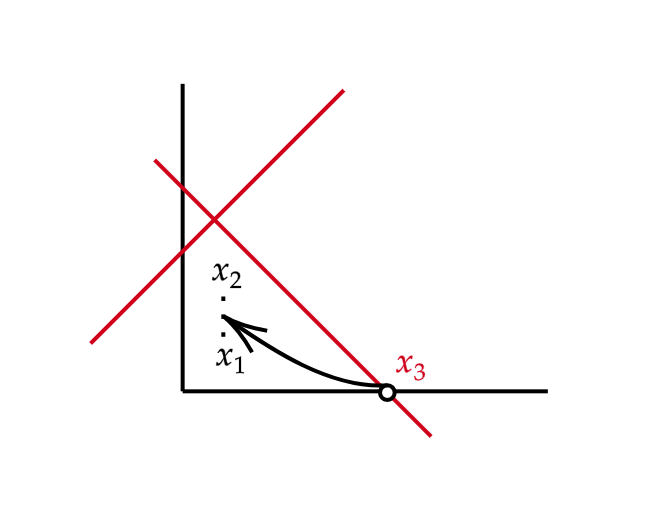
\includegraphics[width=\textwidth]{fig-29.png}
	\end{center}
		
	\noindent \textbf{Recall: } A convex combination is a linear combination of points where all coefficients are non-negative and sum to 1. Moreover, there is always an optimal solution that is basic.
\end{marginfigure}

\begin{thm}
	The \texttt{Rounding} algorithm is a \textbf{2-approximation algorithm} for the weighted Vertex Cover Problem. The integer program is,
	\[
	\begin{array}{lll}
		\operatorname{minimize} & \sum_{i \in V(G)} c_i \cdot x_i & \\
		\text{ subject to } & x_i + x_j \geq 1 & \quad \forall (i, j) \in E(G) \\
		& x_i \in\{0,1\} & \quad \forall i \in V(G)
	\end{array}
	\]
	\noindent but it requires exponential time to solve. Relaxing to a linear program,
	\[
	\begin{array}{lll}
		\operatorname{minimize} & \sum_{i \in V(G)} c_i \cdot x_i & \\
		\text{ subject to } & x_i + x_j \geq 1 & \quad \forall (i, j) \in E(G) \\
		& x_i \in [0,1] & \quad \forall i \in V(G)
	\end{array}
	\]
	\noindent we output $C := \{i \in V \mid x_i \geq \frac{1}{2}\}$.
\end{thm}

\begin{proof}
	\texttt{Rounding} is a 2-approximation algorithm if,
	\begin{enumerate}
		\item It outputs a feasible vertex cover $C$
		\item It runs in polynomial time
		\item Its cost is at most $2 \cdot \texttt{OPT}$
	\end{enumerate}
	\noindent \texttt{Rounding} clearly runs in polynomial time since we have applied relaxation. We need to show that the algorithm outputs a feasible vertex cover. Consider any edge $(i,j) \in E(G)$. By the linear programming constraints, $x_i + x_j \geq 1$, so,
	\[\max\left\{x_{i}, x_{j}\right\} \geq \frac{1}{2}\left(x_{i}+x_{j}\right) = \mu\]
	\noindent and at least one endpoint of $(i,j)$ is in $C$.

	To find the approximation guarantee, let $C^*$ be the minimum cost vertex cover in $G$. $\hat{x}$ is a feasible linear programming solution if\footnote{The optimal solution is feasible.},
	\begin{align*}
	 	\hat{x}_{i}= \begin{cases}1 & i \in C^{*} \\ 0 & i \not\in C^{*}\end{cases}
	 \end{align*}

	\noindent The optimal relaxed linear programming solution $x$ satisfies,
	\[c\left(x\right)=\sum_{i \in V} c_{i} x_{i} \leq \sum_{i \in V} c_{i} x^*_{i} = \texttt{OPT}\]

	\noindent This gives that,
	\begin{align*}
		c(C) &= \sum_{i : x_i \geq 1/2} c_i \\
			 &\leq \sum_{i : x_i \geq 1/2} c_i (2 x_i) \text{ since $2 x_i \geq 1$}\\
			 &\leq 2 \cdot \sum_{i \in V} c_i x_i \\
			 &= 2 \cdot \texttt{OPT}
	\end{align*}
\end{proof}

\begin{thm}
	The linear program for Vertex Cover is $1/2$-integral. That is, any basic solution $\Vec{x}$ satisfies that $x_i \in \{0,1/2,1\}$.
\end{thm}

\begin{proof}
	Let $\Vec{x}$ be a basic solution to our linear program. We can assume that $\Vec{x}$ is fractional, i.e., $0 < x_i < 1$. Suppose not. Then,
	\begin{enumerate}
		\item $x_i = 1$ for some $i \in V$. Select $i \in C$ and consider $G - i$.
		\item $x_i = 0$ for some $i \in V$. Discard $i \in C$ and consider $G - i$\footnote{Any edge with $x_i$ satisfies that its other endpoint is assigned a value of $1$. This follows from the constraints of our integer program, i.e., $x_i + x_j \geq 1$.}
	\end{enumerate}
	\noindent We need to prove that any $x_i$ with a fractional value is $1/2$. 
	\begin{align*}
		V^+ &:= \{i \mid x_i > 1/2\} \\
		V^- &:= \{i \mid x_i < 1/2\} \\
		V^{1/2} &:= \{i \mid x_i = 1/2\} \\
	\end{align*}
	\noindent Observe that $\Vec{x} = \frac{1}{2}(\Vec{y} + \Vec{z})$, where $y_i$ and $z_i$ are defined as follows,
	\[y_{i}=\begin{cases}
			x_{i} & i \in V^{1/2} \\
			x_{i}+\delta & i \in V^{+} \\
			x_{i}-\delta & i \in V^{-}
			\end{cases}
	\quad\quad
	 z_{i} = \begin{cases}x_{i} & i \in V^{1/2} \\
			x_{i}-\delta & i \in V^{+} \\
			x_{i}+\delta & i \in V^{-}\end{cases}\]
	\noindent so $\Vec{x}$ is a convex combination of $\Vec{y}$ and $\Vec{z}$. We will show that $\Vec{y}$ and $\Vec{z}$ are feasible solutions to obtain a contradiction. There can be no edges within $V^-$ or between $V^-$ and $V^{1/2}$ since the constraint $x_1 + x_j \geq 1$ would not be satisfied. The only edges that we can have are,
	\begin{enumerate}
	 	\item $E_1$, between $V^-$ and $V^+$
	 	\item $E_2$, between $V^+$ and $V^{1/2}$
	 	\item $E_3$, within $V^+$ 
	 	\item $E_4$, within $V^{1/2}$
	 \end{enumerate} 
	 \noindent This implies that $\Vec{y}$ is feasible for the linear program,
	 \begin{enumerate}
	 	\item $(i,j) \in E_1$, then $y_i + y_j = (x_i + \delta) + (x_i - \delta) = x_i + x_j \geq 1$
	 	\item $(i,j) \in E_4$, then $y_i + y_j = x_i + x_j \geq 1$
	 	\item $(i,j) \in E_2$, then $y_i + y_j = x_i + (x_j - \delta) = x_i + x_j - \delta \geq 1$
	 	\item $(i,j) \in E_3$, then $y_i + y_j = (x_i - \delta)  + (x_j - \delta) = x_i + x_j - 2\delta \geq 1$
	 \end{enumerate}
	 \noindent since edges in $E_2$ and $E_3$ are such that $x_i + x_j > 1$. Hence, we can choose $\delta$ so that $y_i + y_j \geq 1$. The case for the feasibility of $\Vec{z}$ is analogous. Thus, $\Vec{x} = \frac{1}{2}(\Vec{y} + \Vec{z})$, where $\Vec{y}$ and $\Vec{z}$ are feasible. This is a contradiction unless $\Vec{y} = \Vec{z}$, but then $V^- = V^+ = \emptyset$ so $x_i \in \{0,1/2,1\}$.
\end{proof}

\begin{cor}
	Every basic solution is integral for a bipartite graph.
\end{cor}

\begin{proof}
	Take a basic solution $\Vec{x}$. We proved that $x_i \in \{0,1/2,1\}$, and we can reduce to the case where $\Vec{x}$ is all-fractional. Defining $\Vec{x} = \frac{1}{2}(\Vec{y} + \Vec{z})$, where $y_i$ and $z_i$ and $L, R$ are the bipartitions of $G$,
	\[y_{i}=\left\{\begin{array}{l}
	x_{i}+\delta \quad i \in L \\
	x_{i}-\delta \quad i \in R
	\end{array} \quad z_i =\left\{\begin{array}{l}
	x_{i}-\delta \quad i \in R \\
	x_{i}+\delta \quad i \in L
	\end{array}\right.\right.\]
	\noindent Every edge has one endpoint in $L$ and the other in $R$, 
	\begin{enumerate}
		\item $y_i + y_j = (x_i + \delta) + (x_j - \delta) = x_i + x_j \geq 1$
		\item $z_i + z_j = (x_i - \delta) + (x_j + \delta) = x_i + x_j \geq 1$
	\end{enumerate}
	\noindent implying that $L = R = \emptyset$. Hence, there are no vertices with $x_i = 1/2$. This implies that $\Vec{x}$ is integral, that is, $x_i \in \{0,1\}$.
\end{proof}

\begin{cor}
	Vertex cover is polynomial for a bipartite graph\footnote{We have a 1-approximation algorithm for bipartite graphs.}.
\end{cor}

\begin{thm}
	There is a \textbf{$3/2$-approximation algorithm} for the Vertex Cover Problem in a planar graph.
\end{thm}

\begin{proof}
	Solve the linear program relaxation to obtain a solution $\Vec{x}$ that is $1/2$-integral. Let $V^1 := \{i \mid x_i = 1\}$ and $V^{1/2} := \{i \mid x_i = 1/2\}$. The subgraph of $G$ with vertex set $V^{1/2}$ is planar. By the Four Color Theorem, it can be partitioned into four stable sets, $Q_1, Q_2, Q_3, Q_4$.
	\[V^1 \cup Q_1 \cup Q_2 \cup Q_3\]
	\noindent is a vertex cover\footnote{This effectively takes everything except $V^0$ and $Q_4$, but no edges bridge them by the linear program constraints.}. The linear programming solution is $\sum_{i \in V} c_i \cdot x_i$. Without loss of generality, assume that,
	\[\sum_{i \in Q_4} c_{i} x_{i} \geq \sum_{i \in Q_l} c_{i} x_{i} \quad \quad \forall l=\{1,2,3\}\]
	\noindent But $x_i = 1/2$ for all $i \in \cup_i Q_i$. Hence,
	\[\sum_{i \in Q_4} c_i \geq \sum_{i \in Q_l} c_i \quad \quad \forall l=\{1,2,3\}\]
	\noindent This makes the cost of the algorithm,
	\begin{align*}
	&c(A)=\sum_{i \in V^1} c_{i}+\sum_{i \in Q_1 \cup Q_2 \cup Q_3} c_{i}\\
	&\leq \sum_{i \in V^1} c_{i} \cdot x_{i} + \frac{3}{4} \cdot \sum_{i \in Q_1 \cup Q_2 \cup Q_3 \cup Q_4} c_{i}\\
	&\leq \frac{3}{2} \cdot \sum_{i=V} c_{i} x_{i} \\
	&\leq \frac{3}{2} \cdot \texttt{OPT}
	\end{align*}
	\noindent Thus, we have a $3/2$-approximation algorithm for planar graphs\footnote{The second last inequality follows because the cost of the relaxed program is less than the cost of integer one.}.
\end{proof}

\subsection{Application 4: Set Cover}
We are given $n$ elements $V = \{v_1, \cdots, v_n\}$ and $m$ sets $S_1, \cdots, S_m \subseteq V$ with costs $c_1, \cdots, c_m$. The goal is to find a minimum cost collection of sets that cover every element in $V$. This problem is NP-Complete.

\begin{thm}[Greedy Set Cover]
	\texttt{GreedySet} is a \textbf{$O(\log n)$-approximation algorithm} for the Set Cover Problem. The algorithm is greedy.
\end{thm}

\begin{algorithm}
	  \caption{Greedy Algorithm for Set Cover}\label{setcovergreedy}
	  \Function{GreedySet($X$, $S$)}{
	  \Comment{$U$ stores the uncovered elements}
	  $U \assign X$\;
	  \Comment{$C$ stores the sets of the cover}
	  $C \assign \emptyset$\;
	  \While{$U \neq \emptyset$}{
	  		\Comment{Select the set $S_j^*$ which covers the remaining uncovered elements at a minimum average cost}
		  	$S_j \assign S_j^*$\;
		  	$C \assign C \cup S_j$\;
		  	$U \assign U - S_j^*$\;
	  	}
	    \Return{$C$}\;
	  }
\end{algorithm}

\begin{marginfigure}
	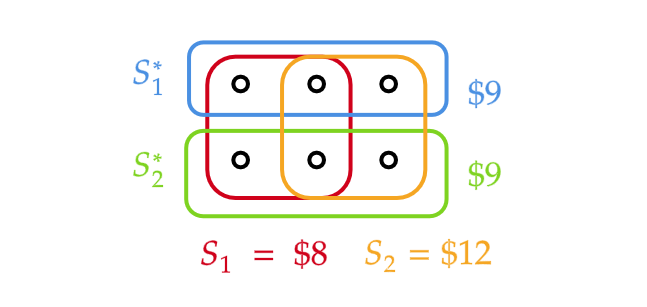
\includegraphics[width=\textwidth]{fig-30.png}
	\caption{Illustration of \texttt{GreedySet}. Sets are sorted by average cost, where the average is taken over cardinality.}
\end{marginfigure}

\begin{proof}
	The algorithm clearly runs in polynomial time and outputs a feasible set cover. We need to prove that $\alpha = O(\log n)$. Let,
	\begin{align*}
		&\texttt{OPT} := \{S^*_1, \cdots, S_k^*\}
		&\underbrace{C := \{S_1, \cdots, S_r\}}_{r \text{ possibly } \neq k}
	\end{align*}
	\noindent and $C$ as the output of \texttt{GreedySet}. We want to prove that,
	\[\sum_{j=1}^r c(S_j) \leq \log n \cdot \sum_{j=1}^k c(S_j^*)\]

	Label the elements of $V$ by $\{1, 2, \cdots, n\}$, based on the order that they are covered by \texttt{GreedySet}. Let $U_t$ be the set of uncovered elements at the start of step $t$\footnote{$U_1 = V$ and $U_t \subset U_{t-1}$.}. If $S_t$ is the set selected by \texttt{GreedySet} at $t$, then $n_t = |S_t \cap U_t|$ is the number of new elements covered at $t$.

	\noindent If $i \in S_t \cap U_t$, then $i$ was covered at step $t$. Then,
	\[\alpha_i = \frac{c(S_t)}{n_t}\]

	\noindent is the cost of covering $i$. Hence, $\sum_{t=1}^{k} c(S_{t})=\sum_{i=1}^{n} \alpha_{i}$. To see this,
	\begin{align*}
		\sum_{t=1}^{r} c(S_{t}) &= \sum_{t=1}^{r} \alpha_i \cdot n_t \\
								&= \sum_{i=1}^{n}  \alpha_i \quad \text{(where $|V| = n$)}\\
	\end{align*}

	To analyze the cost of \texttt{GreedySet}, it suffices to bound $\alpha_i$. When $i$ was covered, there were at least $n - i + 1$ uncovered elements. \texttt{OPT} can cover all of these elements for an average cost of,
	\[\frac{1}{n-i+1} \cdot \left(\sum_{i=1}^{k} c(S_i^*)\right)=\frac{1}{n-i+1} \cdot \texttt{OPT}\]

	Since $S_t$ must do at least as well as this, $\alpha_i \leq \frac{1}{n-i+1} \cdot \texttt{OPT}$,
	\begin{align*}
		\sum_{i=1}^{n}  \alpha_i &\leq \sum_{i=1}^{n} \frac{1}{n-i+1} \cdot \texttt{OPT} \\
								 &= \texttt{OPT} \cdot \sum_{i=1}^{n} \frac{1}{n-i+1} \\
								 &= \texttt{OPT} \cdot \sum_{l=1}^n \frac{1}{l} \\
								 &= \texttt{OPT} \cdot H_n
	\end{align*}
	\noindent where $H_n \approx \log n$ is the $n$th partial sum of a Harmonic series. Thus,
	\[c(\{S_1, \cdots, S_r\}) \leq O(\log n) \cdot \texttt{OPT}\]
\end{proof}

\begin{ex}{Proof of Tighteness}{label}
	Suppose that all sets have cost \$1. Then,
	\begin{align*}
		&c(\texttt{OPT}) = c(\{S_1^*, S_2^*\}) = 2\\
		&c(C) = c(\{S_1, \cdots, S_r\}) =  r
	\end{align*}
	\begin{center}
		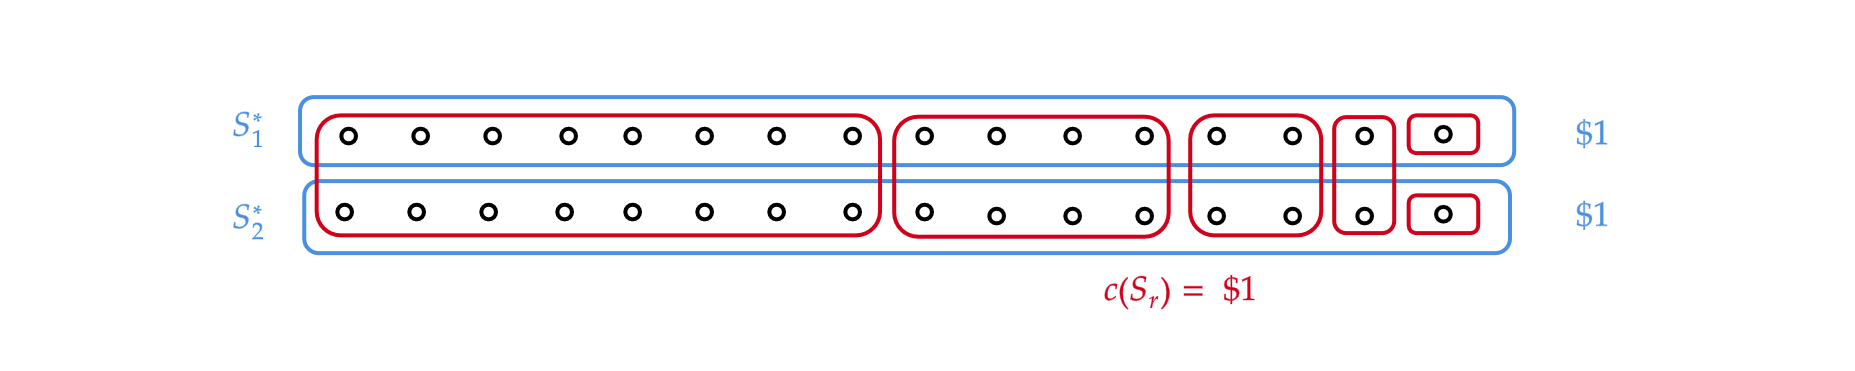
\includegraphics[width=\textwidth]{fig-31.png}
	\end{center}
	\noindent But, $r = \Omega\left(\log n \right)$ so $n = 2 + \sum_{j=1}^{r-1} 2^j$.
\end{ex}

\begin{rmk}
	There is no $\alpha$-approximation for the Set Cover Problem with $\alpha = c \cdot \log n$ and $c < 1$ unless $P = NP$. We will not see the proof of this.
\end{rmk}

\subsection{Application 5: Hitting Set}
We are given $m$ elements $E = \{1, 2, \cdots, m\}$ with respective costs $c_1, c_2, \cdots, c_m$ and sets $T_1, T_2, \cdots T_n \subseteq E$. The goal is to find a minimum cost set of elements that "hit" every set $T_1, \cdots, T_n$.

\begin{rmk}
	Since the Hitting Set Problem is equivalent to the Set Cover Problem, we can use \texttt{GreedySet} to solve it.
\end{rmk}

\begin{defn}[Randomized Rounding]
	Let $T_j$ be the indices of the sets $S_j$ that cover element $i$. The integer problem to solve Hitting Set uses a randomized rounding algorithm,
		\[
		\begin{array}{lll}
			\operatorname{minimize} & \sum_{j=1}^m c_i \cdot x_i & \\
			\text{ subject to } & \sum_{j \in T_i} x_j \geq 1 & \quad \forall T_i\\
			& x_i \in\{0,1\} & \quad \forall i \in V(G)
		\end{array}
		\]
	\noindent and it can be relaxed as follows,
	\[
		\begin{array}{lll}
			\operatorname{minimize} & \sum_{j=1}^m c_i \cdot x_i & \\
			\text{ subject to } & \sum_{j \in T_i} x_j \geq 1 & \quad \forall T_i\\
			& x_i \in [0,1] & \quad \forall i \in V(G)
		\end{array}
	\]
	\noindent where element $j$ is selected with probability $x_j$.
\end{defn}

\begin{rmk}
	The expected cost of the randomized algorithm is,
	\[\sum_{j=1}^{m} c_{j} x_{j} = \texttt{LP} \leq \texttt{OPT}\]
	\noindent where \texttt{LP} is the value of our linear program. While the algorithm is polynomial, it may not output a feasible solution.
\end{rmk}

\begin{marginfigure}
	\textbf{Arithmetic-Mean Inequality: }

	\noindent For any $\alpha_1 \cdots \alpha_k \geq 0$,
	\[\frac{\sum_{i} \alpha_{i}}{k} \geq \sqrt[k]{\pi \alpha_{i}}\]
\end{marginfigure}

\begin{rmk}
	If $X_i$ be the event that $T_i$ is hit, then $P(X_i) \geq 1 - \frac{1}{e}$.
\end{rmk}

\begin{proof}
	Put $T_i := \{1, 2, \cdots, k\}$. By the linear programming constraints, $\sum_{j=1}^k x_j \geq 1$. Hence, the probability that $T_i$ is missed is,
	\begin{align*}
		P(X_i^c) &= \prod_{j=1}^k (1 - x_j) \\
				 &= \prod_{j=1}^k \alpha_j \\
				 &\leq \left(\frac{1}{k} \cdot (\alpha_1 + \cdots + \alpha_k\right)^k \\
				 &= (1 - \frac{1}{k} \cdot \sum x_j)^k \\
				 &\leq (1 - \frac{1}{k})^k \text{ since $\sum x_j \geq 1$}
	\end{align*}
	\noindent But, $(1 - \frac{1}{k})^k \leq \frac{1}{e} = \lim_{n \rightarrow \infty} \left(1 - \frac{1}{n}\right)^n$. Thus, the probability that $T_i$ is hit is strictly bigger than $\frac{1}{2}$.
\end{proof}

\begin{cor}
	Our solution may miss half the sets. If the algorithm is run $\ell = 2 \log n$ times, then the probability of missing a set is reduced to $\frac{1}{n}$\footnote{Consequently, with high probability, randomized rounding gives a hitting set with cost $\leq 2 \log n \cdot \texttt{OPT}$.}.
\end{cor}

\subsection{Application 6: Maximum Satisfiability}
Let $x_1, x_2, \cdots, x_n$ be boolean variables. Recall that,
\begin{enumerate}
	\item A positive literal is a variable $x_i$
	\item A negative literal is a negation $\bar{x_i}$.
	\item A clause is a disjunction of literals
\end{enumerate}
The goal is to assign the variables \texttt{True} and \texttt{False} while satisfying as many as clauses possible.

\begin{thm}
	Independently assigning each variable $x_i$ to be \texttt{True} with probability $1/2$ is a $1/2$-approximation algorithm.
\end{thm}

\begin{proof}
	Take a clause $C_j$ with $k$ literals. $C_j$ is not satisfied with probability $\frac{1}{2^k}$. Therefore, $C_j$ is satisfied with probability $1 - \frac{1}{2^k}$. The worst case occurs when $k = 1$, but $1 - \frac{1}{2^k} \geq \frac{1}{2}$. This means that each clause is satisfied with a probability of at least $\frac{1}{2}$. Let $m$ be the total number of clauses. By linearity of expectation, the expected number of satisfied clauses is at least $\frac{1}{2} \cdot m \geq \frac{1}{2} \cdot \texttt{OPT}$.
\end{proof}

\begin{rmk}
	This is a $7/8$-approximation algorithm for Maximum 3-SAT because each clause is satisfied with probability $1 - \frac{1}{2^3} = \frac{7}{8}$\footnote{In fact, unless P = NP, there is no better approximation algorithm.}.
\end{rmk}

\begin{thm}[Randomized Satisfiability]
	The following integer program solves the Maximum Satisfiability Problem,
	\[
		\begin{array}{lll}
			\operatorname{maximize} & \sum_{j=1}^m z_i & \\
			\text{ subject to } & \sum_{x_i \in C_j} y_j + \sum_{x_i \in C_j} (1 - y_i) \geq z_j & \quad \forall j\\
			& y_i, z_j\in\{0,1\} & \quad \forall i, j
		\end{array}
	\]
	\noindent where clauses are indexed by $j$, variables are indexed by $i$, and each clause $C_j$ corresponds to $z_j$. To see that this works\footnote{The clause constraint is satisfied if and only if at least one of the literals are assigned correctly.}, let, 
	\[
	y_{i}=\left\{\begin{array}{ll}
	1 & \text { if } x_{i}=\texttt{True} \\
	0 & \text { if } x_{i}=\texttt{False}
	\end{array} \quad z_{j}= \begin{cases}1 & \text { if } C_{j} \text { satisfied } \\
	0 & \text { if } C_{j} \text { not satisfied }\end{cases}\right.
	\]
	\noindent We solve the linear program relaxation in polynomial time with $0 \leq y_i \leq 1$ and $0 \leq z_i \leq 1$ for all $i, j$. To do this, set $x_i = \texttt{True}$ with probability $y_i$.
\end{thm}

\begin{marginfigure}
	\textbf{Recall: } If $f(x)$ is concave on $[0,1]$ with $f(0) = t$ and $f(1) = a + b$, then, \[f(x) \geq ax + b\]
\end{marginfigure}

\begin{proof}
	Since $C_j$ has $k$ literals, it is satisfied with minimum probability,
	 \[\left(1 + \left(1 + \frac{1}{k}\right)^k\right) \cdot z_j\]
	 \noindent We will prove this using the Arithmetic Mean Inequality. Without loss of generality, let $C_j \ x_1 \lor x_2 \lor \cdots \lor x_k$. Then,
	\begin{align*}
		\prod_{j=1}^k (1 - y_i) &\leq \left(\frac{\sum (1-y_i)}{k} \right)^k \text{ by the Arithmetic Mean Inequality}\\
								&= \left(1 - \frac{\sum y_i}{k}\right)^k \\
								&\leq \left(1 - \frac{z_j}{k}\right)^k \text{ by the constraint $\sum_{x_i \in C_j} y_i \geq z_j$}
	\end{align*}
	\noindent is the probability that $C_j$ is not satisfied. Note that $g(x) = \left(1 - \frac{x}{k}\right)^k$ is convex, and consequently $f(x) = 1 - g(x)$ is concave. Thus,
	\begin{enumerate}
		\item $f(0) = (1 - 0)^k = 0 = b$
		\item $f(1) = (1 - \frac{1}{k})^k = a + b = a$ since $b = 0$
	\end{enumerate}
	\noindent Hence, the probability that $C_j$ is satisfied is greater than,
	\[a \cdot z_j = \left(1 - \frac{1}{k}\right)^k \cdot z_j\]
	\noindent but we have seen that this gives a guarantee of $\frac{1}{e}$. Thus,
	\[\geq \underbrace{\left(1 - \frac{1}{e}\right)}_{\approx 0.632} \cdot z_k\]
	\noindent The expected number of clauses satisfied is greater than or equal to,
	\[\sum_j 0.632 \cdot z_j \geq 0.632 \cdot \sum_j z_j \geq 0.632 \cdot \sum_j \texttt{OPT}\]
	\noindent since $\sum_j z_j$ is our objective function.
\end{proof}

\begin{thm}
	Taking the best out of the previous two approximation algorithms, $\mathcal{R}_1$ and $\mathcal{R}_2$, gives a $3/4$-approximation algorithm.
\end{thm}

\begin{proof}
	Let $N_1$ and $N_2$ be the number of clauses satisfied by $\mathcal{R}_1$ and $\mathcal{R}_2$, respectively. Simplifying and applying induction with,
	\begin{align*}
		\mathbb{E}[\max \{N_1, N_2\}] &\geq \mathbb{E}\left[\frac{1}{2} \cdot (N_1 + N_2)\right] \text{ since $\max \geq \mu$}\\
								     &= \frac{1}{2} \cdot \mathbb{E}[N_1] + \mathbb{E}[N_2] \text{ by linearity of expectation}
	\end{align*}
	\noindent gives the result. The complete proof is not shown.
\end{proof}

\begin{rmk}
	In fact, we can get a $3/4$ guarantee using non-linear randomized rounding. We solve the linear program to find $y_i$ and $z_i$, and set $x_i = \texttt{True}$ with probability $f(y_i)$. This works if the function $f$ satisfies,
	\[1 - \frac{1}{4^y} \leq f(y) \leq f^{y-1}\]
\end{rmk}

\begin{proof}
	The probability that $C_j$ is satisfied is,
	\begin{align*}
	1-\prod_{x_{i} \in C_{j}}\left(1-f\left(y_{i}\right)\right) \cdot \prod_{\bar{x}_{i} \in C_{j}} f\left(y_{i}\right)
	&\geq 1-\prod_{x_{i} \in C_{j}}\left(1-\left(1-\frac{1}{4 y_{i}}\right)\right) \cdot \prod_{\bar{x}_{i} \in C_{j}} 4^{y_{i}-1} \\
	&=1-\prod_{x_{i} \in C_{j}} \frac{1}{4 y_{i}} \cdot \prod_{\bar{x}_{i} \in C_{j}} 4^{y_{i}-1}\\
	&=1-4^{-\sum_{x_{i} \in C_{j}} y_{i}+\sum_{\bar{x}_{i} \in C_{j}}\left(y_{i}-1\right)}\\
	&=1-4^{-\left(\sum_{x_{i} \in C_{j}} y_{i}+\sum_{\bar{x}_{i} \in C_{j}}\left(1-y_{i}\right)\right)}\\
	&\geq 1 - 4^{2j} \text{ by our constraints}
	\end{align*}
	\noindent Using concavity, $f(z_j) \geq \frac{3}{4} \cdot z_j$.
\end{proof}

\begin{ex}{Proof of Tightness}{label}
	This analysis is tight with respect to the upper bound,
	\begin{enumerate}
		\item $C_1 = x_1 \lor x_2$
		\item $C_2 = x_1 \lor \bar{x}_2$
		\item $C_3 = \bar{x_1} \lor x_2$
		\item $C_4 = \bar{x_1} \lor \bar{x_2}$
	\end{enumerate}

	Moreover, it is tight with respect to \texttt{OPT},
	\begin{enumerate}
		\item $C_1 = x_1 \lor x_2$
		\item $C_2 = x_1 \lor \bar{x_2}$
		\item $C_3 = \bar{x_1} \lor x_2$
		\item $C_4 = \bar{x_1} \lor \bar{x_3}$
	\end{enumerate}
\end{ex}

\subsection{Application 7: Steiner-Tree Problem}
\begin{defn}[Steiner-Tree Problem]
	Suppose that we are given a graph $G = (V, E)$ with edge costs $c_e \geq 0$ and a set $R \subseteq V$ of terminals. The goal is to find a minimum cost subgraph $T$ that connects all the terminals. This subgraph is called a \textbf{Steiner tree}. The non-terminals are called \textbf{Steiner nodes}, and they are only used if they reduce the cost of the tree\footnote{Remark that the leaves of a Steiner tree are necessarily terminals.}.
\end{defn}

\begin{cor}
	If $R = V(G)$, then this is the minimum spanning tree problem. If $R \subset V(G)$, then the problem is NP-Complete.
\end{cor}

 \begin{thm}
 	\texttt{SteinerApprox} is a 2-approximation algorithm.
 \end{thm}

\begin{algorithm}
	  \caption{2-Approximation Algorithm for Steiner Trees}\label{steineralgo}
	  \Function{SteinerApprox($X$, $S$)}{
	  \Comment{For terminals $r_1, r_2$, let $P_{ij}$ be the shortest path between them. Denote its length by $\ell_{ij}$}
	  $P_{ij} \assign \delta(i,j)$\;
	  \Comment{Construct an auxiliary graph $H$ that is a complete graph on the set of terminals. Let $(i,j) \in H$ have cost $\ell_{ij}$}
	  $T \assign \FuncCall{Prim}{$H$, $\ell$}$\;
	  \Return{$\bigcup_{(i,j) \in T} P_{ij}$}\;
	  }
\end{algorithm}

% https://courses.cs.duke.edu/cps296.5/current/scribing/cps590_lec16-17.pdf

 \begin{proof}
 	\texttt{SteinerApprox} is a 2-approximation algorithm if,
	\begin{enumerate}
		\item It outputs a feasible vertex cover $C$
		\item It runs in polynomial time
		\item Its cost is at most $2 \cdot \texttt{OPT}$
	\end{enumerate}
	\noindent \texttt{SteinerApprox} is polynomial, and it outputs a feasible solution. Let $T^*$ be the optimal Steiner tree. We can walk around the outside of $T^*$ to create a circuit $C$. This circuit can be divided into paths,
	\[C = Q_1 \cup Q_2 \cup \cdots \cup Q_k\]
	\noindent where $Q_i$ is the path from $r_i$ to $r_{i+1}$. Thus,
	\[c(C) = 2 \cdot c(T^*) = \sum_{i=1}^k c(Q_i)\]
	\noindent but the path $P = \{r_1, \cdots, r_k\}$ is a spanning tree in $H$. Thus,
	\begin{align*}
		c(F) &\leq c(P) \\
			 &= \sum_{i=1}^{k-1} \ell_{i,i+1} \\
			 &\leq \sum_{i=1}^{k-1} Q_i \\
			 &\leq \sum_{i=1}^k c(Q_i) \\
			 &= 2 \cdot \texttt{OPT}
	\end{align*}
	\noindent Since we return $T^{\prime} = \bigcup_{(i,j) \in T} P_{ij}$, we have,
	\[C(T^{\prime}) \leq c(F) \leq 2 \cdot \texttt{OPT}\]
 \end{proof}

\subsection{Application 8: Knapsack Problem}
Suppose that we are given a bag with capacities $w$ and $n$ objects, where each object $i$ has weight $w_i$ and value $v_i$. The goal is to find the subset of items of maximum value that fit in the Knapsack. We saw that this can be formulated as an integer program,
\[\begin{array}{ll}
		\operatorname{maximize} & \sum_{i=1}^{n} v_{i} \cdot x_{i} \\
		\text{ subject to } & \sum_{i=1}^{n} w_{i} \cdot x_{i} \leq W \\
		& x_{i} \in\{0,1\} \quad \forall i \in[n]
\end{array}\]

\begin{lem}
	For a basic solution $\Vec{x}$, there is at most one item with,
	\[0 < x_i < 1\]
\end{lem}

\begin{proof}
	Recall the Greedy Algorithm for the Knapsack Problem,
	\begin{enumerate}
		\item Compute the value per weight $V_i := v_i / w_i$ for each item
		\[\frac{v_1}{w_1} \geq \frac{v_2}{w_2} \geq \cdots \geq \frac{v_n}{w_n}\]
		\item Iterating through the sorted list, put,
		\[
		x_i^G = \begin{cases}
			1 & \text{if $i$ fits completely} \\
			0 & \text{if the knapsack is full} \\
			\frac{W - \sum_{l=1}^{i-1} w_l}{w_i} & \text{otherwise}
		\end{cases}
		\]
	\end{enumerate}
	\noindent After the first fractional item $0 < x_k^G < 1$, the bag is full. Thus,
	\begin{align*}
		\Vec{x}^G &= \left(x_1^G, \cdots, x_{k-1}^G, x_k^G, x_{k+1}^G, \cdots x_n^G\right) \\
				  &= \left(1, \cdots, 1, 1, x_k^G, \cdots 0, \cdots, 0\right)
	\end{align*}
	\noindent An exchange argument shows that $\Vec{x}^G$ is the optimal solution. Assume for a contradiction that it is not. Then some items before $k$ are used below 1. Re-assign weight from $x_j$ to $x_i$, where $i < k \leq j$ by setting,
	\begin{align*}
		&x_j \leftarrow x_j - \delta \\
		&x_i \leftarrow x_i + \frac{\delta \cdot w_j}{w_i}
	\end{align*}
	to save $\delta \cdot w_j$ in weight. The change in value is,
	\[-\delta \cdot v_{j}+\delta \cdot \frac{w_{j}}{w_{j}} \cdot v_{i}=\delta \cdot w_{j} \cdot\left(\frac{v_{i}}{w_{i}}-\frac{v_{i}}{w_{j}}\right) \geq 0\]
	\noindent as $i$ has a better "bang-for-buck" than $j$. We can repeat this until we obtain $\Vec{x}^G$, but this means that $\Vec{x}^G$ is an optimal basic solution\footnote{The solution is basic because it only has one fractional value.}.
\end{proof}

\begin{rmk}
	This gives the following polynomial \texttt{BestOfTwo} algorithm,
	\begin{enumerate}
		\item Solve the linear programming relaxation
		\item Output the maximum value subset between,
		\[I_1 := \{i \mid x_i = 1\} \quad I_2 := \{i \mid 0 < x_i < 1\}\]
	\end{enumerate}
	\noindent where $I_1$ and $I_2$ are both feasible solutions,
	\begin{enumerate}
		\item $I_1$ is feasible since it has weight $\leq W$
		\item $I_2$ is feasible since each weight is less than the size of the bag\footnote{If not, then we can remove this item and recurse to obtain a solution with the same properties.}
	\end{enumerate}
\end{rmk}

\begin{proof}
	\texttt{BestOfTwo} is a 2-approximation algorithm because,
	\begin{align*}
		\max \{v(I_1), v(I_2)\} &\geq \frac{1}{2} \cdot \left(v(I_1) + v(I_2)\right) \\
								&= \frac{1}{2} \sum_{i=1}^n v_i \\
								&\geq \frac{1}{2} \sum_{i=1}^n v_i \cdot x_i \\
								&\geq \frac{1}{2} \cdot \texttt{OPT}
	\end{align*}
\end{proof}

\begin{defn}[Approximation Scheme]
	An algorithm $\mathcal{A}$ is a \textbf{fully polynomial time approximation scheme} for a maximization problem if, 
	\begin{enumerate}
		\item $\mathcal{A}$ outputs a solution of value $\geq (1 - \epsilon) \cdot \texttt{OPT}$
		\item $\mathcal{A}$ runs in time polynomial in $|\texttt{I}|$ and $\frac{1 }{\epsilon}$
	\end{enumerate}
	\noindent for any instance \texttt{I} and $\epsilon > 0$.
\end{defn}

\begin{thm}
	There is a fully polynomial time approximation scheme for the Knapsack Problem. It is based on dynamic programming.
\end{thm}

\begin{proof}
	Let $w(i, V)$ be the minimum weight of a subset of the items $[i]$ of value $\geq V$. This is by convention infinite if the value of $[i]$ is less than $V$. The dynamic program can be solved recursively as $w(i, V) = \min \{w(i-1,V), w_i + w(i-1, V - v_i)\}$ with base cases $w(i, V) = 0$ for all $V \leq 0$. Let $V_{\max} := \max_i v_i$. Then there are $n$ choices for $i$ and at most $n \cdot V_{\max}$ choices for $V$. This means that there are $O(n^2 \cdot V_{\max})$ subproblems, solvable in $O(2)$.

	Since $V_{\max}$ can be exponential in the number of bits, this is a pseudo-polynomial time algorithm. We can resolve this by scaling down each value without substantially losing accuracy. 
\end{proof}

\subsection{Parameterized Complexity}
\begin{defn}[Fixed-Parameter Tractable]
	A problem is \textbf{fixed parameter tractable} if it has an algorithm to solve it that runs in time $f(k) \cdot \text{poly}(n)$, where $n$ is the problem input size, $k$ is the size of the optimal solution, and $f$ need not be a polynomial function.
\end{defn}

\begin{ex}{Vertex Cover}{label}
	If we are given that the optimal solution $C^*$ to the Vertex Cover Problem has \text{$k$} vertices, then we can check in \text{$O\left(m \cdot \binom{n}{k}\right) = O(m \cdot n^k)$} if a subset \text{$C$} is a vertex cover.

	This running time is exponential in the size of the optimal solution, not in the input size. It serves as a motivating example for the question: \textit{Can we separate the time dependency on $n$ and $k$ completely?} Specifically, we want an algorithm in,
	\[O(\text{poly}(n) \cdot f(k))\]
	\noindent where $f(k)$ is exponential, or worse, in $k$. If we can do this, then the problem is called \textbf{fixed parameter tractable}.
\end{ex}

\begin{lem}
	Let $M^*$ be a maximum matching and $C^*$ be a minimum vertex cover in a non-bipartite graph. Then,
	\[\left|M^{*}\right| \leq\left|C^{*}\right| \leq 2 \cdot\left|M^{*}\right|\]
\end{lem}

\begin{proof}
	Let $M^* := \{e_1, e_2, \cdots, e_l\}$, where $e_i = (u_i, v_i)$. Then $V - V(M^*)$ is an independent set in $G$\footnote{If not, then we could construct a larger matching than $M^*$.}. Moreover, $V(M^*)$ is a vertex cover. This means that the minimum vertex cover $C^*$ is at most the size of $C$,
	\[\left|C^{*}\right| \leq|C|=2 \cdot l=2 \cdot\left|M^{*}\right|\]
\end{proof}

\begin{thm}
	% Vertex Cover is fixed-parameter tractable.
	Let $G$ be a non-bipartite graph with minimum vertex cover $C^*$ of size $k$. Then, $C^*$ can be found in time $3^k \cdot \text{poly}(n)$.
\end{thm}

\begin{proof}
	Find a maximum matching $M^* = \{e_1, \cdots, e_l\}$ in polynomial time. Observe that $l \leq k$, or else $|C^*| \geq k$. At least one endpoint $e_i = (u_i, v_i)$ is in $C^*$, so there are three possibilities for $e_i$,
	\begin{align*}
		&u_{i} \in C^{*} \wedge v_{i} \notin C^{*} \\
		&u_{i} \notin C^{*} \wedge v_{i} \in C^{*} \\
		&u_{i} \in C^{*} \wedge v_{i} \in C^{*}
	\end{align*}
	\noindent This gives $3^l$ possibilities, producing subsets $C_1, \cdots, C_{3^l}$. Moreover, we know that there exists $j$ such that $C_j = C^* \cap V(M^*)$. To find the correct index $j$, we can try every possibility. There are two cases,
	\begin{enumerate}
		\item There is an edge $e$ whose endpoints are both in $V(M^*) - C_j$. Then it cannot be covered by adding vertices of $V - M^*$ to $C_j$. Thus, this is not the correct choice and we can reject it.
		\item There are no edges whose endpoints are both in $V(M^*) - C_j$. Any edge $e$ incident to a vertex in $C_j$ is already covered. Since $V - M^*$ is an independent set, any other edge $f$ has one endpoint in $V(M^*) - C_j$ and the other in $V - V(M^*)$. To cover these edges, we select a vertex in $V - V(M^*)$ as $C_j$ are the only vertices in $V(M^*)$ that touch at least one edge uncovered by $C_j$. Let $W_j$ be the set of vertices in $V - V(M^*)$ that touch at least one edge uncovered by $C_j$. Thus, $\hat{C}_j = C_j \cup W_j$ is the smallest vertex cover $C$ such that,
		\[\hat{C}_j = C_j \cup W_j\]
		\noindent We output the smallest $\hat{C}_j$, which is the minimum vertex cover.
	\end{enumerate}
	We conclude that the total running time is at most,
	\[3^l \cdot \text{poly}(n) \leq 3^k \cdot \text{poly}(n)\]
\end{proof}

We can repeat the same procedure for the Longest Path Problem.

\begin{thm}
	Suppose that the longest path $P^*$ contains exactly $k$ vertices,
	\[P^* = \{v_1, v_2, \cdots, v_k\}\]
	\noindent We can find $P^*$ exhaustively in $O(k \cdot n^k)$ by,
	\begin{enumerate}
		\item Taking every possible sequence $P$ of $k$ vertices
		\item Testing if $P$ is a path
	\end{enumerate}
\end{thm}

In fact, we can do better. A useful technique in the design of fixed parameter tractable algorithms is the color coding method.

\begin{defn}[Color Coding]
	The \textbf{color coding method} colors each object in the search space, so that the algorithm can refine its search for monochromatic or panchromatic solutions.
\end{defn}

\begin{rmk}
	The color coding method applies to the Longest Path Problem.
\end{rmk}

\begin{proof}
	Assume the longest path is $P^* = \{v_1, v_2, \cdots, v_k\}$. Randomly color the vertices of $G$ with $k$ colors. If col($v_i$) $= i$ for all $1 \leq i \leq k$, then we can find $P^*$ in linear time by Breadth-First Search:
	\begin{enumerate}
		\item Begin with vertices of color 1, and search for neighbors in color 2
		\item From these neighbors, search for neighbors of neighbors of color 3
		\item Repeat this procedure until color $k$
	\end{enumerate}
	\noindent The probability that $v_i$ is given color $i$ is $\frac{1}{k}$, so the probability that every vertex in $P^*$ is given the correct color is,
	\[\left(\frac{1}{k}\right)^k\]
	Suppose that the color coding algorithm is run $t$ times. Each run is independent, so the probability of failure every time is at most,
	\[\left(1-\left(\frac{1}{k}\right)^{k}\right)^{t}=\left(1-\frac{1}{k^{k}}\right)^{t}\]
	\noindent Using the fact that $1-x<e^{-x} \quad \forall x \neq 0$,
	\[\left(1-\frac{1}{k^{k}}\right)^{t} \leq\left(e^{-\frac{1}{k^{k}}}\right)^{t}=e^{-\frac{t}{k^{k}}}\]
	\noindent If we try this $t = k^k \cdot \log n$ times, then the probability is at most,
	\[e^{-\frac{t}{k^{k}}}=e^{-\log n}=\frac{1}{n}\]
	\noindent So at least one of the trials succeeds with probability at least $1 - \frac{1}{n}$. Moreover, the algorithm runs in time $k^k \cdot \text{poly}(n)$, making the problem fixed parameter tractable.
\end{proof}














\end{document}